\documentclass[UTF8]{ctexart}
\usepackage{geometry}
\usepackage{amsmath,mathtools,mathdots,extarrows,psfrag,lipsum,array}
\usepackage{xcolor}
\usepackage{tikz,pgfplots,tcolorbox,graphicx}
\usepackage{caption,subcaption}
\usepackage{amssymb}
\usepackage{booktabs}
\usepackage{bm}
\usepackage{enumitem}
\usepackage{pdfpages}
%封面样式
\usepackage{multicol,multirow}
%符合国标gbt7714的引用范式
\usepackage{gbt7714}
%目录的链接
\usepackage[hidelinks]{hyperref}
%cc协议的图案
\usepackage[scale=1]{ccicons}
%脚注的圆圈序号
\usepackage{pifont}
%常用的图案,用于区分定理、例题结束的标记
\usepackage{typicons}

%宏包{breqn}和tikz包{tikzmark}相互冲突,使用前者后会在后者的命令下反复报错'pgf cannot find shape a'之类。
%%%%%%%%%%%%%%new command environment%%%%%%%%%%%%
\newcommand{\onech}[4]{
\makebox[92pt][l]{(A) #1} \hfill
\makebox[92pt][l]{(B) #2} \hfill
\makebox[92pt][l]{(C) #3} \hfill
\makebox[92pt][l]{(D) #4}\\}

\allowdisplaybreaks

\newcommand*\enumlabel[1]{
    \tikz[baseline=(char.base)]{\node[shape=rectangle,inner sep=2pt,fill=Blue] (char) {{\textcolor{white}{#1}}};
    }
}

\newcommand*\enulabel[1]{
    \tikz[baseline=(char.base)]{\node[shape=rectangle,inner sep=2pt] (char) {{\textcolor{Blue}{#1}}};
    }
}

\newcommand*\zheng{
    \tikz[baseline=(char.base)]{\node[shape=rectangle,inner sep=0pt] (char) {{\bfseries\heiti\textcolor{Light_Yellow}{证明:\quad}}};
    }
}

\newcommand*\jie{
    \tikz[baseline=(char.base)]{\node[shape=rectangle,inner sep=0pt] (char) {{\bfseries\heiti\textcolor{Blue}{解:\quad}}};
    }
}

\newenvironment{Quotation}[1]
    {\newcommand\quotesource{#1}
    \begin{quotation}}
    {\par\hfill\sffamily\bfseries\setlength\leftskip{2em} ——\quotesource
    \end{quotation}}

%%%%%%%%%%%%%%%%%%graphic settings%%%%%%%%%%%%%%%%
\tcbuselibrary{external,breakable,skins}
\usetikzlibrary{decorations.pathreplacing,positioning,shapes.misc,decorations.markings,calc,intersections,arrows.meta,graphs,shapes.misc,decorations.pathmorphing,decorations.shapes,tikzmark,angles,quotes,patterns}
\bibliographystyle{gbt7714-numerical}
\geometry{a4paper,centering,scale=0.8,left=2cm,right=2cm,bottom=2cm,top=2.5cm}

%脚注设置
\renewcommand\thefootnote{\ding{\numexpr171+\value{footnote}}}

%目录链接设置
\hypersetup{
    colorlinks=false,
    citecolor=black,
    filecolor=black,
    urlcolor=black
}

\tikzset{every picture/.style={>=Latex}}
%%%%%%%%%%%%%%%%%%%fonts settings%%%%%%%%%%%%%%%%%
\setmainfont{Times New Roman}
\setsansfont{Georgia}
\setmonofont{Arial}

%%%%%%%%%%%%%%%%%%chapter settings%%%%%%%%%%%%%%%%
\ctexset{
    section={
    format+=\sectionFormat,
    titleformat=\tcblower,
    aftertitle=\end{tcolorbox}
    },
    subsection={
    format+=\sectionFormatt,
    titleformat=\tcblower,
    aftertitle=\end{tcolorbox}
    },
    subsubsection={
    format+=\sectionFormattt,
    titleformat=\tcblower,
    aftertitle=\end{tcolorbox}    
    }
    }
\newcommand\sectionFormat[1]{
\begin{tcolorbox}[colback=Cream_4!10,
    colframe=white,leftrule=0mm,sharp corners,toprule=0mm,bottomrule=0mm,rightrule=0mm,sidebyside,lefthand ratio=0.1,colupper=Blue,collower=Blue,fontupper=\LARGE,fontlower=\LARGE,lower separated=false]
#1
}
\newcommand\sectionFormatt[1]{
\begin{tcolorbox}[colback=white,
    colframe=white,leftrule=0mm,sharp corners,toprule=0mm,bottomrule=0mm,rightrule=0mm,sidebyside,lefthand ratio=0.05,colupper=Blue,collower=Blue,fontupper=\Large,fontlower=\Large,lower separated=false,size=minimal,beforeafter skip=1em]
#1
}
\newcommand\sectionFormattt[1]{
\begin{tcolorbox}[colback=white,
    colframe=white,sharp corners,leftrule=0mm,toprule=0mm,bottomrule=0mm,rightrule=0mm,sidebyside,lefthand ratio=0.05,colupper=Blue,collower=Blue,fontupper=\large,fontlower=\large,lower separated=false,size=minimal,beforeafter skip=1em]
#1
}
%%%%%%%%%%%%%%%%%tcolorbox settings%%%%%%%%%%%%%%%
%备注:1.每定义一个新的\newtcolorbox都可以在使用环境的时候输入若干个参数。如果参数是在\begin……\end{}中用中括号[]加入的话,在定义的时候{name}[nums]后要加入一个空白的中括号,表示接受来自引用时的参数,如\newtcolorbox{pr}[1][],第一个中括号内表示参数的个数。如果使用环境时的参数不是以中括号[]而是以大括号{}加入的话,定义环境时就不要放入中括号,直接在用#1表示参数即可。使用中括号传递参数的好处是,如果使用环境时不一定传递该参数,将默认该参数为空。但是用大括号使用环境时必须使用{}传递参数,否则将默认环境内容的第一个字符为该参数,造成不必要的混淆。当传递两个参数时,大括号{}传递一个具体的参数值,而中括号[]传递一个参数设置,定义环境时先定义中括号[]的内容,即#1,使用环境时中括号放在前面。2.在如下定义的prf环境中,框线是根据 title box 的定位去画的,所以在使用prf环境的时候,可以不传递参数,也就是标题,但会导致框线不显示,因为没有 title box。3.enhanced选项很重要,很多功能的实现需要依靠它。

\newtcolorbox{prf}[1][]{fonttitle=\bfseries\heiti,colback=white,coltitle=white,breakable,enhanced,attach boxed title to top left={xshift=10mm},sharp corners,title={证明},after title={#1},size=fbox,after upper=\hfill$\blacksquare $,frame hidden,boxed title style={colback=Vintage_3,colframe=Vintage_3,sharp corners},
overlay unbroken={
    \draw[Vintage_3,line width=0.5mm] (title.west) -- ([yshift=\tcboxedtitleheight/2]frame.north west) -- (frame.south west) -- (frame.south east);},
overlay first={
    \draw[Vintage_3,line width=0.5mm] (title.west) -- ([yshift=\tcboxedtitleheight/2]frame.north west) -- (frame.south west);},
overlay middle={
    \draw[Vintage_3,line width=0.5mm] (frame.north west)--(frame.south west);},
overlay last={
    \draw[Vintage_3,line width=0.5mm] (frame.north west)--(frame.south west)--(frame.south east);}
}

\newtcolorbox{theorem}[1][]{fonttitle=\bfseries\heiti,colback=white,frame hidden,breakable,title=#1,enhanced,attach boxed title to top left={xshift=10mm},sharp corners,
boxed title style={coltitle=white,colback=Blue,colframe=Blue,sharp corners},
overlay unbroken={
    \draw[Blue,line width=0.5mm] (title.west) -- ([yshift=\tcboxedtitleheight/2]frame.north west) -- (frame.south west) -- (frame.south east);},
overlay first={
    \draw[Blue,line width=0.5mm] (title.west) -- ([yshift=\tcboxedtitleheight/2]frame.north west) -- (frame.south west);},
overlay middle={
    \draw[Blue,line width=0.5mm] (frame.north west)--(frame.south west);},
overlay last={
    \draw[Blue,line width=0.5mm] (frame.north west)--(frame.south west)--(frame.south east);}
}

\newtcolorbox[auto counter,number within=section]{definition}[1][]{enhanced,frame hidden,colback=white,coltitle=Blue,fonttitle=\bfseries,title={定义~\thetcbcounter},detach title,before upper={\tcbtitle\quad},after title={\quad#1},breakable,sharp corners,borderline west={1mm}{0mm}{Cream_3}}

\newtcolorbox{case}{enhanced,colframe=Lake_Blue!10,colback=Lake_Blue!10,sharp corners,breakable,borderline west={1mm}{0mm}{Lake_Blue}}

\newtcolorbox[auto counter,number within=section]{liti}[1][]{colback=white,coltitle=Blue,frame hidden,breakable,before skip=1cm,title=错题回顾 \thetcbcounter,enhanced,attach boxed title to top left,sharp corners,fonttitle=\LARGE\heiti,
boxed title style={empty,colframe=Blue,size=minimal,overlay={\draw[Blue,line width=2pt]([yshift=2pt]frame.north west)--([yshift=2pt]frame.north east);}},
overlay unbroken={
    \draw[Blue,line width=1pt] ([yshift=2pt]title.north west) -- ([yshift=\tcboxedtitleheight+2pt]frame.north east);
    \draw[Blue,line width=1pt] (frame.south west)--(frame.south east);},
overlay first={
    \draw[Blue,line width=1pt] ([yshift=2pt]title.north west) -- ([yshift=\tcboxedtitleheight+2pt]frame.north east);},
overlay last={
    \draw[Blue,line width=1pt] (frame.south west)--(frame.south east);}
}

\newtcbox{\txe}{on line,arc=1pt,colback=Blue!10,colframe=white,colupper=Blue,boxrule=0pt,boxsep=0pt,left=5pt,right=3pt,top=2pt,bottom=2pt}

\newtcolorbox[auto counter]{examp}[1][]{enhanced,frame hidden,colback=white,coltitle=Blue,fonttitle=\bfseries,title={例~\thetcbcounter},detach title,before upper={\tcbtitle},after title={\quad#1},breakable,sharp corners,size=minimal,
overlay unbroken={
    \node [yshift=0.5em] at (frame.south east) {\Large\color{Blue}\tiPinOutline};},
overlay last={
    \node [yshift=0.5em] at (frame.south east) {\Large\color{Blue}\tiPinOutline};}}

\newtcolorbox[auto counter]{ttheorem}[1][]{enhanced,frame hidden,colback=white,coltitle=Blue,title={\bfseries 定理~\thetcbcounter},detach title,before upper={\tcbtitle},after title={\heiti#1\quad},breakable,sharp corners,beforeafter skip=0.5em,size=minimal,
overlay unbroken={
    \node [yshift=0.5em] at (frame.south east) {\Large\color{Blue}\tiLightbulb};},
overlay last={
    \node [yshift=0.5em] at (frame.south east) {\Large\color{Blue}\tiLightbulb};}}

%%%%%%%%%%%%%%%%%%Color Definition%%%%%%%%%%%%%%%%
\definecolor{Light_Yellow}{HTML}{CF7F19}
\definecolor{Light_Green}{HTML}{007C63}
\definecolor{Lake_Blue}{HTML}{7192C5}
\definecolor{Blue}{HTML}{2e9ce9}
%Nature
\definecolor{Nature_1}{HTML}{F4FCD9}
\definecolor{Nature_2}{HTML}{C5D8A4}
\definecolor{Nature_3}{HTML}{BB9981}
\definecolor{Nature_4}{HTML}{534340}
%Vintage
\definecolor{Vintage_1}{HTML}{E5E3C9}
\definecolor{Vintage_2}{HTML}{B4CFB0}
\definecolor{Vintage_3}{HTML}{94B49F}
\definecolor{Vintage_4}{HTML}{789395}
%Cream
\definecolor{Cream_1}{HTML}{F7FBFC}
\definecolor{Cream_2}{HTML}{D6E6F2}
\definecolor{Cream_3}{HTML}{B9D7EA}
\definecolor{Cream_4}{HTML}{769FCD}

\title{Notes for Mathematics$^{\, \ccbync}$}
\author{可达可达}
\date{}

\begin{document}
\includepdf{123.pdf} 
\newpage
\maketitle
\tableofcontents

\zihao{-4}
\section{前言}
本来洋洋洒洒落笔千言,最后删减到现在的三言两语,我还是决定把最纯粹的内容奉献给大家。我写这份笔记,一方面是个人学习的总结,便于不断地复习回顾;另一方面也是希望能够给那些在学习数学上遇到困难的同道中人一些微不足道的帮助;最后,比较详尽的公式让那些有教学、科研需要的朋友们可以到源文件内直接复制粘贴,大大减轻了他们的工作量,也能更加美观。本笔记错误、疏漏在所难免,希望大家谅解。

这份笔记是由\LaTeX{}编写的,我认为\LaTeX{}有更自由的方式来实现我偏好的设计,同时其对于数学公式的排版也是诸如Word、Indesign等无法媲美的。在笔记的体例上,大致是正文和特殊环境的组合。特殊环境中,定义被环境左侧的视觉引导线包裹,证明结束的标志是实心的小正方形$\blacksquare $,定理和例题的分别是灯泡和图钉。这样,正文和特殊环境总是能够区分开来。同时,我定义了一系列的命令如:\jie \zheng \txe{注:} 等等来方便录入。笔记的内容参考了本科数学教材、考研教辅资料和真题等等。

另外,本笔记内容(包括.tex源文件)全部开源,并遵循CC协议。

\hfill 可达可达

\hfill 2023年1月2日
\section{高等数学}
\subsection{初等数学提挈}
\subsubsection{常用三角函数公式}
\begin{align*}
    \sin^2 \alpha + & \cos^2\alpha = 1 &
    \tan^2 \alpha + & 1 = \sec^2 \alpha \\
    \cot \alpha  & =\frac{1}{\tan \alpha} &
    \cot^2 \alpha + & 1 = \csc^2 \alpha \\
    \csc \alpha & =\frac{1}{\sin \alpha} &
    \sec \alpha & = \frac{1}{\cos \alpha} 
\end{align*}
\begin{enumerate}
\item 两角和差公式
\begin{gather*}
    \sin(\alpha+\beta)=\sin\alpha\cos\beta+\cos\alpha\sin\beta \\
    \sin(\alpha-\beta)=\sin\alpha\cos\beta-\cos\alpha\sin\beta \\
    \cos(\alpha+\beta)=\cos\alpha\cos\beta-\sin\alpha\sin\beta \\
    \cos(\alpha-\beta)=\cos\alpha\cos\beta+\sin\alpha\sin\beta\\
    \tan(\alpha+\beta)=\frac{\tan\alpha+\tan\beta}{1-\tan\alpha\tan\beta}\\
    \tan(\alpha-\beta)=\frac{\tan\alpha-\tan\beta}{1+\tan\alpha\tan\beta}
\end{gather*}
\item 积化和差公式
\begin{align*}
    \sin \alpha \cos \beta & =\frac{1}{2}[\sin (\alpha+\beta)+\sin(\alpha-\beta)]  \\
    \cos \alpha \sin \beta & =\frac{1}{2}[\sin (\alpha+\beta)-\sin(\alpha-\beta)]  \\
    \cos \alpha \cos \beta & =\frac{1}{2}[\cos (\alpha+\beta)+\cos(\alpha-\beta)]  \\
    \sin \alpha \sin \beta & =-\frac{1}{2}[\cos (\alpha+\beta)-\cos(\alpha-\beta)]
\end{align*}
\item 和差化积公式
\begin{align*}
    \sin\alpha+\sin\beta & =2\sin\frac{\alpha+\beta}{2}\cos\frac{\alpha-\beta}{2}  \\
    \sin\alpha-\sin\beta & =2\cos\frac{\alpha+\beta}{2}\sin\frac{\alpha-\beta}{2}  \\
    \cos\alpha+\cos\beta & =2\cos\frac{\alpha+\beta}{2}\cos\frac{\alpha-\beta}{2}  \\
    \cos\alpha-\cos\beta & =-2\sin\frac{\alpha+\beta}{2}\sin\frac{\alpha-\beta}{2} \\
    \tan\alpha+\tan\beta & =\frac{\sin (\alpha+\beta)}{\cos\alpha\cdot\cos \beta}
\end{align*}
\item 倍角公式
\begin{align*}
    \cos 2\alpha & =\cos^2 \alpha-\sin^2\alpha=2\cos^2\alpha-1=1-2\sin^2\alpha\\
    \sin 2\alpha  & =2\sin \alpha \cos \alpha\\
    \tan 2\alpha  & =\frac{2\tan\alpha}{1-\tan^2\alpha}, \tan\alpha=\frac{\sin2\alpha}{1+\cos2\alpha}=\frac{1-\cos2\alpha}{\sin2\alpha}
\end{align*}
\end{enumerate}

\subsubsection{排列组合}
$A_n^m$表示从$n$个不同的元素中取出$m$个元素的排列;

$C_n^m$表示从$n$个不同的元素中取出$m$个元素的组合.
\begin{align*}
    0!&=1 & 
    n!&=n\cdot (n-1)\cdot (n-2) \dots 2\cdot 1\\
    A_n^m&=\frac{n!}{(n-m)!} & 
    C_n^m&=\frac{n!}{m!\times (n-m)!}\\
\end{align*} 
二项式定理:
\begin{align*}
    (a+b)^n&=\sum^{n}_{k=0}\mathbf{C} _n^ka^{n-k}b^k \\
    &=a^n+na^{n-1}b+\frac{n(n-1)}{2!}a^{n-2}b^2\\
    &+\dots+\frac{n(n-1)\dots(n-k+1)}{k!}a^{n-k}b^k+\dots+nab^{n-1}+b^n.
\end{align*}

因式分解:
\begin{align*}
    a^3+b^3=(a+b)(a^2-ab+b^2)\\
    a^3-b^3=(a-b)(a^2+ab+b^2)\\
\end{align*}

\subsubsection{常见的几种初等函数图像及其性质}

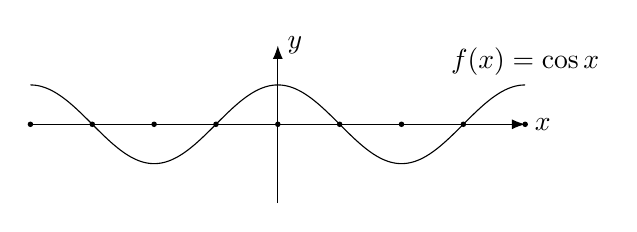
\begin{tikzpicture}[scale=0.5,smooth,samples=100]
    \draw[->](-2*pi,0) -- (2*pi,0) node[right] {$x$};
    \draw[->](0,-2) -- (0,2) node[right] {$y$};
    \foreach \x in {-2,-3/2,-1,-0.5,0,0.5,1,1.5,2}
        {\fill (\x*pi,0) circle (2pt);
        }
    \draw [domain=-2*pi:2*pi] plot (\x,{cos(\x r)}) node[above] {$f(x) = \cos x$};
\end{tikzpicture}
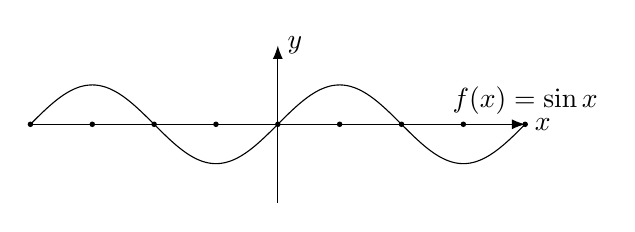
\begin{tikzpicture}[scale=0.5,smooth,samples=100]
    \draw[->](-2*pi,0) -- (2*pi,0) node[right] {$x$};
    \draw[->](0,-2) -- (0,2) node[right] {$y$};
    \foreach \x in {-2,-3/2,-1,-0.5,0,0.5,1,1.5,2}
        {\fill (\x*pi,0) circle (2pt);
        }
    \draw [domain=-2*pi:2*pi] plot (\x,{sin(\x r)}) node[above] {$f(x) = \sin x$};
\end{tikzpicture}

\begin{tikzpicture}[scale=0.5,smooth,samples=100]
    \draw[->](-2*pi,0) -- (2*pi,0) node[right] {$x$};
    \draw[->](0,-5) -- (0,5) node[right] {$y$};
    \foreach \x in {-2,-3/2,-1,-0.5,0,0.5,1,1.5,2}
        {\fill (\x*pi,0) circle (2pt);
        }
    \draw [domain=-2*pi+0.2:-pi-0.2] plot (\x,{cot(\x r)});
    \draw [domain=-pi+0.2:-0.2] plot (\x,{cot(\x r)});
    \draw [domain=0.2:pi-0.2] plot (\x,{cot(\x r)});
    \draw [domain=pi+0.2:2*pi-0.2] plot (\x,{cot(\x r)}) node[below] {$f(x) = \cot x$};
\end{tikzpicture}
\begin{tikzpicture}[scale=0.5,smooth,samples=100]
    \draw[->](-2*pi,0) -- (2*pi,0) node[right] {$x$};
    \draw[->](0,-5) -- (0,5) node[right] {$y$};
    \foreach \x in {-2,-3/2,-1,-0.5,0,0.5,1,1.5,2}
        {\fill (\x*pi,0) circle (2pt);
        }
    \draw [domain=-2*pi+0.2:-pi-0.2] plot (\x,{1/sin(\x r)});
    \draw [domain=-pi+0.2:-0.2] plot (\x,{1/sin(\x r)});
    \draw [domain=0.2:pi-0.2] plot (\x,{1/sin(\x r)});
    \draw [domain=pi+0.2:2*pi-0.2] plot (\x,{1/sin(\x r)}) node[below] {$f(x) = \csc x$};
\end{tikzpicture}

\begin{tikzpicture}[scale=0.5,smooth,samples=100]
    \draw[->](-2*pi,0) -- (2*pi,0) node[right] {$x$};
    \draw[->](0,-5) -- (0,5) node[right] {$y$};
    \foreach \x in {-2,-3/2,-1,-0.5,0,0.5,1,1.5,2}
        {\fill (\x*pi,0) circle (2pt);
        }
    \draw [domain=-2*pi:-1.5*pi-0.2] plot (\x,{1/cos(\x r)});
    \draw [domain=-1.5*pi+0.2:-0.5*pi-0.2] plot (\x,{1/cos(\x r)});
    \draw [domain=-0.5*pi+0.2:0.5*pi-0.2] plot (\x,{1/cos(\x r)});
    \draw [domain=0.5*pi+0.2:1.5*pi-0.2] plot (\x,{1/cos(\x r)});
    \draw [domain=1.5*pi+0.2:2*pi] plot (\x,{1/cos(\x r)}) node[right] {$f(x) = \sec x$};
\end{tikzpicture}
\begin{tikzpicture}[scale=0.5,smooth,samples=100]
    \draw[->](-5,0) -- (5,0) node[right] {$x$};
    \draw[->](0,-3) -- (0,3) node[right] {$y$};
    \draw [domain=-5:5] plot (\x,{ln(\x+sqrt(1+\x*\x))}) node[above] {$f(x)=\ln(x+\sqrt{1+x^2})$};
\end{tikzpicture}

\subsubsection{解方程}
\begin{examp}{$
    \begin{dcases}
        \sin x_0+a\cos x_0=a+\frac{1}{2}\\
        \tan x_0 =\frac{1}{a}.
    \end{dcases}$其中$a$为常数,求$a$.}
    
    \jie 将二式代入一式消去$\sin x$,化简后画三角形解方程:
    \begin{gather*}
        \begin{dcases}
            \cos x_0=\frac{a^2+\frac{1}{2}a}{a^2+1},\\
            \tan x_0 =\frac{1}{a}.
        \end{dcases}
        \hfill
        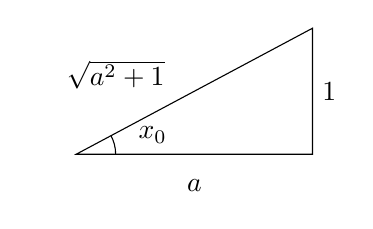
\begin{tikzpicture}[baseline=(char.base)]
            \node(char) at (0,0) {};
            \draw(0.5,-0.8) coordinate (A)--(3.5,-0.8) coordinate (B)--(3.5,0.8) coordinate (C)--cycle pic ["$x_0$",draw,angle radius=0.5cm,angle eccentricity=2] {angle = B--A--C};
            \node (cha) at ($(0.5,-1)!0.5!(3.5,-1)$) [below] {$a$};
            \node (cha) at ($(3.5,-0.8)!0.5!(3.5,0.8)$) [right] {$1$};
            \node (cha) at ($(0.5,-1)!0.5!(3.5,0.8)$) [above,xshift=-1cm] {$\sqrt{a^2+1}$};
        \end{tikzpicture}\\
        \implies \cos x_0=\frac{a}{\sqrt{a^2+1}}=\frac{a^2+\frac{1}{2}a}{a^2+1}
        \implies a=\frac{3}{4}
    \end{gather*}
\end{examp}

\subsubsection{不等式}
\begin{figure}[htp]
\centering
\begin{tikzpicture}
    \matrix 
    {
    \node(a1){调和平均值}; & & \node(a2){几何平均值}; & & \node(a3){算术平均值}; & & \node(a4){平方平均值}; \\
    \node(b1){$\dfrac{2}{\dfrac{1}{x}+\dfrac{1}{y}}$}; & \node{$\leqslant$}; & \node(b2){$\sqrt{xy} $}; & \node{$\leqslant$}; & \node(b3){$\dfrac{x+y}{2} $}; & \node{$\leqslant$}; & \node(b4){$\sqrt{\dfrac{x^2+y^2}{2}}$}; \\
    };
\end{tikzpicture}
\end{figure}
一个更一般的结论:
\begin{align*}
    \frac{n}{\sum\limits^{n}_{i=1}\frac{1}{a_i}}\leqslant \sqrt[n]{\prod^n_{i=1}a_i} \leqslant\frac{\sum\limits^{n}_{i=1}a_i}{n} \leqslant \sqrt{\frac{\sum\limits^{n}_{i=1}a_i^2}{n}}
\end{align*}

与绝对值有关的不等式:
\begin{align*}
    \left\lvert a\pm b\right\rvert \leqslant & \left\lvert a\right\rvert +\left\lvert b\right\rvert .&
    \left\lvert \left\lvert a\right\rvert -\left\lvert b\right\rvert \right\rvert \leqslant & \left\lvert a-b\right\rvert. \\
    \left\lvert a_1\pm a_2\pm \dots\pm a_n\right\rvert  \leqslant & \left\lvert a_1\right\rvert +\left\lvert a_2\right\rvert + \dots \left\lvert a_n\right\rvert. &
    \left\lvert \int_{b}^{a} f(x) \,\mathrm{d}x \right\rvert \leqslant & \int_{b}^{a} \left\lvert f(x)\right\rvert  \,\mathrm{d}x.\\
    \frac{1}{x+1}<\ln \left(1+\frac1x \right) < & \frac{1}{x} ,(x>0). &
    \left\lvert ab\right\rvert \leqslant & \frac{a^2+b^2}{2}.
\end{align*}
\begin{prf}
    \begin{gather*}
        \sqrt{ab} \leqslant\frac{a+b}{2}\implies \sqrt{a^2b^2} =\left\lvert ab\right\rvert \leqslant\frac{a^2+b^2}{2}
    \end{gather*}
\end{prf}
证明不等式的问题有两种思路,一种是把问题转化为函数$f(x)$在定义域内恒大于或小于0;另一种是比较不等式两边的函数在定义域内的最大值和最小值的问题,适用于不等式两边过于复杂的情况
\begin{examp}{证明:$\left(\ln \frac{1+x}{x}-\frac{1}{1+x}\right) ^2<\frac{1}{x(1+x)^2},(x>0).$}
\end{examp}

证明两个变量的不等式的思路是要么把两个变量化成一个,要么把其中一个变量当作常数化为恒成立问题,这是通用的方法.但合适的时候使用拉格朗日中值定理大大方便了证明.

\begin{examp}{设$0<a<b,$证明:$\ln \frac{b}{a}>2\frac{b-a}{a+b}.$}
    \par \jie 把不等式右边化为$\frac{\frac{b}{a}-1}{\frac{b}{a}+1}.$
\end{examp}
证明积分不等式有一个常用的方法,构造积分变限函数,可令:
\begin{equation*}
    (a-b)f(x)=\int_{a}^{b} f(x) \,\mathrm{d}t \text{或} f(x)\int_{a}^{b}  \,\mathrm{d}t .
\end{equation*}
\begin{examp}{设$f(x)$在$[a,b]$上连续,且$f(x)>0$.证明:$\int_{a}^{b} f(x) \,\mathrm{d}x \cdot \int_{a}^{b} \frac{1}{f(x)} \,\mathrm{d}x \geqslant (b-a)^2.$}
    \par \zheng 令$F(x)=\int_{a}^{x} f(t) \,\mathrm{d}t \cdot \int_{a}^{x} \frac{1}{f(t)} \,\mathrm{d}t -(x-a)^2, 0 \leqslant x \leqslant b. \\
    F'(x)=f(x)\int_{a}^{x} f(t) \,\mathrm{d}t +\int_{a}^{x} \frac{1}{f(t)} \,\mathrm{d}t \cdot \frac{1}{f(x)} =\int_{a}^{x} \left( \frac{f(x)}{f(t)}+\frac{f(t)}{f(x)}-2 \right) \,\mathrm{d}t \geqslant 0,\\
    F(x)$单调递增,故$F(b)> F(a)=0$.
\end{examp}
\begin{examp}{设$f(x)$在$[0,1]$上连续,且单调递减.证明:当$0<\lambda<1$时,$\int_{0}^{\lambda} f(x) \,\mathrm{d}x \geqslant \lambda \int_{0}^{1} f(x) \,\mathrm{d}x .$}
    \par \zheng 观察到右边$\int_{0}^{1} f(x) \,\mathrm{d}x $是一个常数,故把$\lambda$移到左边.要证$\int_{0}^{\lambda} f(x) \,\mathrm{d}x \geqslant \lambda \int_{0}^{1} f(x) \,\mathrm{d}x $,只要证$\frac{\int_{0}^{\lambda} f(x) \,\mathrm{d}x }{\lambda}\geqslant \int_{0}^{1} f(x) \,\mathrm{d}x $,令$F(\lambda)=\frac{\int_{0}^{\lambda} f(x) \,\mathrm{d}x }{\lambda},\\ 
    F'(\lambda)=\frac{f(\lambda)\cdot \lambda-\int_{0}^{\lambda} f(x) \,\mathrm{d}x }{\lambda^2}=\frac{f(\lambda)\int_{0}^{\lambda}  \,\mathrm{d}x -\int_{0}^{\lambda} f(x) \,\mathrm{d}x }{\lambda^2}=\frac{\int_{0}^{\lambda} [f(\lambda)-f(x)] \,\mathrm{d}x }{\lambda^2}<0,\\
    F(\lambda)$单调递减,故$F(\lambda) > F(1) = \int_{0}^{1} f(x) \,\mathrm{d}x $,即$\int_{0}^{\lambda} f(x) \,\mathrm{d}x \geqslant \lambda \int_{0}^{1} f(x) \,\mathrm{d}x .$
\end{examp}
\begin{examp}{设$0<a<b<1,$证明:$\arctan b-\arctan a<\frac{b-a}{2ab}.$}
    \par \zheng 构造$f(x)=\arctan x.$由拉格朗日中值定理,存在$\xi \in (a,b),f'(\xi)=\frac{f(b)-f(a)}{b-a}\implies \frac{1}{1+\xi^2}=\frac{\arctan b-\arctan a}{b-a},\frac{1}{1+\xi^2}<\frac{1}{1+a^2}<\frac{1}{b^2+a^2}<\frac{1}{2ab}\implies \arctan b-\arctan a<\frac{b-a}{2ab}.$
\end{examp}

\subsection{极限}
\subsubsection{求取极限的几种重要方法}
\begin{enumerate}
    \item 两个重要的极限:
\begin{align*}
    \lim_{x \to 0}\frac{\sin x}{x}=1,\\
    \lim_{x \to \infty}\left(1+\frac{1}{x}\right)^x=\mathrm{e}.
\end{align*}

由第二个重要极限可以推出,若$\lim u^v$属于$1^\infty$型,那么
\begin{equation*}
    \lim u^v=\mathrm{e}^{\lim (u-1)v}.
\end{equation*}

\begin{prf}
    \begin{gather*}
        \lim u^v=\lim \left[(u-1+1)^{\frac{1}{u-1}}\right]^{(u+1)v}=\mathrm{e}^{\lim (u-1)v}
    \end{gather*}
\end{prf}

\item 等价无穷小量替换

当$x\to 0$时,几个重要的等价无穷小量替换:
\begin{align*}
    \sin x &\sim x & \tan x &\sim x\\
    \arcsin x &\sim x & \arctan x &\sim x\\
    \ln(1+x) &\sim x & e^x-1 &\sim x\\
    a^x-1 &\sim x\ln a & 1-\cos x &\sim \frac{1}{2}x^2\\
    (1+x)^\alpha-1 &\sim \alpha x & (1+x)^\alpha-1 &\sim \alpha x
\end{align*}

当$x \to x_0 $时,若$f(x) \to 0, g(x) \to 0,$则有$\mathrm{e}^{f(x)}-\mathrm{e}^{g(x)}\sim f(x)-g(x).$

\txe{注:$\mathrm{e}^{\tan x}-\mathrm{e}^{x}\sim \tan x-x.$}

\zheng $\mathrm{e}^{f(x)}-\mathrm{e}^{g(x)}=\mathrm{e}^{f(x)}(1-\mathrm{e}^{g(x)-f(x)})\sim -\mathrm{e}^{f(x)}(g(x)-f(x))\sim f(x)-g(x).$\hfill$\blacksquare $

当$f(x) \to 0,g(x) \to 1 $时,若出现$\mathrm{e}^{f(x)}$或$\ln g(x)$,则要考虑进行凑配,将上述式子变成$\mathrm{e}^{f(x)}-1+1$和$\ln [g(x)-1+1]$,由于$x\to 0,\mathrm{e}^x-1\sim x, \ln (x+1)\sim x$,所以$\mathrm{e}^{f(x)}-1+1\sim f(x)+1,\ln [g(x)-1+1]\sim g(x)-1$.

当$f(x)\to 0$,对$a^{f(x)}-1$,都化作$\mathrm{e} ^{{f(x)}\ln a}-1,$.
\begin{examp}
    $2^x-1=\mathrm{e} ^{\ln 2^x}-1=\mathrm{e} ^{x\ln 2}-1=x\ln 2,x\to 0$.
\end{examp}

\begin{ttheorem}
    有界函数和无穷小量的乘积仍为无穷小量.
\end{ttheorem}

\begin{examp}{$\lim_{x \to 0} x^2\cdot\sin \frac{1}{x}=0$}
    
\end{examp}

\begin{examp}{$\lim_{x \to \infty} \frac{2x^2-3}{5x^2+2\sin x}$}

    \jie 构造无穷小量解决$\sin x$.
    
    $\lim_{x \to \infty} \frac{2x^2-3}{5x^2+2\sin x}=\lim_{x \to \infty} \frac{2-\frac{3}{x^2}}{5+\frac{2}{x^2}\sin x}=\frac{2}{5}.$
\end{examp}

\item 泰勒展开

当$x\to 0$时,几个重要的泰勒展开式:
\begin{align*}
    \arcsin x &= x +\frac{x^3}{3!}+o(x^3) & \arctan x &= x -\frac{x^3}{3}+o(x^3)\\
    \tan x &=x+\frac{x^3}{3}+o(x^3) & &
\end{align*}
\txe{注:记忆技巧:tan分母无阶乘,反三角函数符号异,sin与tan符号异.}

使用泰勒公式求极限时,要注意高阶无穷小量是否趋向于0.
\begin{examp}
    {$\lim_{n \to \infty} \frac{\mathrm{e} ^{\frac{1}{n^2}}-\cos \frac{\pi}{n}}{\frac{1}{n^2}},n \to \infty,o(\frac{1}{n}) \to 0.$}
\end{examp}

\begin{examp}
    {$\lim_{n \to \infty} a\cdot \left( \frac{n}{n+1} \right)^n=\lim_{n \to \infty} a\cdot \left( \frac{1}{1+\frac{1}{n}} \right)^n=\lim_{n \to \infty} a\cdot  \frac{1}{\left(1+\frac{1}{n}\right) ^n} =\frac{a}{\mathrm{e} }.$}
\end{examp}

无穷小量的运算规则:
\begin{gather*}
    o(x^m)+o(x^n)=o(x^l),l=\min\left\{m,n\right\} \\
    o(x^m)\cdot o(x^n)=o(x^{m+n}),x^m\cdot o(x^n)=o(x^{m+n})\\
    k\cdot o(x^m)=o(x^m)
\end{gather*}

\item 几个定式:

对于形如$a^x+b^x$式子的处理方法:提取$a^x\left[1+\left(\frac{b}{a}\right) ^x\right] $;

对于形如$a^x+a^y$式子的处理方法:提取$a^x \left(1+a^{y-x} \right)$;

对于形如$a^x+b^y$式子的处理方法:提取$a^x \left(1+\frac{b^y}{a^x} \right)$ .

若$\left\lvert q\right\rvert <1,\lim_{n \to \infty}q^n=0$.

\item 拉格朗日中值定理:


\item 洛必达法则

出现$0/0,\infty/\infty$型的极限采用洛必达法则进行计算,在洛的过程中适当加入等价无穷小量代换可以降低计算难度.

\enumlabel{1.}对于$\infty\pm\infty$型要先观察能否通分化简转换成第一种情况,如果不可以,再观察有无形如$1/x$的变量,然后换元转换成第一种情况;如果既不能通分也不能换元就考虑把所有式子对数化,让后用对数运算法则变为两个数相乘.
\begin{examp}
    {$\lim_{x \to \infty}\left[\ln (\mathrm{e}^x+1)-x \right] = \lim_{x \to \infty}\left[\ln (\mathrm{e}^x+1)+\ln \mathrm{e}^{-x} \right] \\= \lim_{x \to \infty}\ln (\mathrm{e}^x+1)\mathrm{e}^{-x}=0.$}
\end{examp}
\begin{examp}
    {$\lim_{x \to +\infty}(\ln x-\frac{x}{\mathrm{e}}+k)=\lim_{x \to +\infty}(\ln x-\ln e^{x/\mathrm{e}}+k)=\ln \lim_{x \to +\infty}\frac{x}{e^{x/e}}+k=\ln \lim_{x \to +\infty}\frac{e}{e^{x/e}}+k=-\infty+k=-\infty$}
\end{examp}

\enumlabel{2.}对于$0^\infty,\infty^\infty$则将原式化为$\mathrm{e}$的指数再求极限:$u^v=e^{\ln u^v}=e^{v\ln u}.$使用洛必达法则遇到$e^{-x}$要将它放到分母上.
\begin{examp}
    {$\lim_{x \to \infty}x^2e^{-2x}=\lim_{x \to \infty}\frac{x^2}{e^{2x}},\lim_{x \to -\infty}xe^x=\lim_{x \to -\infty}\frac{x}{1/e^x}$.}
\end{examp}

\begin{examp}
    {$\lim_{x \to 0} x^x=1$}
\end{examp}

\begin{examp}{$\lim_{x \to 1^{-}} \frac{1}{x-1}\mathrm{e} ^{\frac{1}{x^2-1}}$}

    \jie 注意$(1^-)^2-1<0,(1^-)^2=1^-$,
    
    $\lim_{x \to 1^{-}} \frac{1}{x-1}\mathrm{e} ^{\frac{1}{x^2-1}}=\lim_{x \to 1^{-}} -\frac{2x}{(x^2-1)^2}\mathrm{e} ^{\frac{1}{x^2-1}}\\
    =\lim_{x \to 1^{-}} 2x\cdot\lim_{x \to 1^{-}} -\frac{1}{(x^2-1)^2}\mathrm{e} ^{\frac{1}{x^2-1}}$,换元,令$t=\frac{1}{x^2-1}$,得$-2 \lim_{t \to -\infty} t^2 \mathrm{e} ^t=-2 \lim_{t \to -\infty} \frac{t^2}{\frac{1}{\mathrm{e} ^t}}=-2 \lim_{t \to -\infty} \frac{2t}{-\frac{1}{\mathrm{e} ^t}}=-2 \lim_{t \to -\infty} \frac{2}{\frac{1}{\mathrm{e} ^t}}=-2 \lim_{t \to -\infty} 2 \mathrm{e} ^t=0$
\end{examp}

\end{enumerate}

\subsubsection{极限的运算法则}
\begin{enumerate}
    \item $\lim \left[k f(x) \pm l g(x)\right] =k\lim f(x)+l\lim g(x)$.
    \item $\lim \left[f(x)\cdot g(x)\right] =\lim f(x)\cdot \lim g(x)$.
\end{enumerate}

形如$\displaystyle \lim_{x \to x_0} \frac{f(x)-g(x)}{h(x)}$的极限:
\begin{enumerate}
    \item 求分数的极限要注意是否是无穷小量比阶,若是无穷小量比阶,当式子中出现加减运算,求极限时不能采用等价无穷小量替换,可以用泰勒展开,也可以用洛必达法则.这是因为等价无穷小量替换的精度太低,往往只展开到一阶,这往往比分母的阶数小,我们可以写出它的高阶无穷小量$o(x)$来比较其与分母的阶数.
    
    \item 若$\lim_{x \to x_0} g(x)=0$,可以用极限的四则运算法则将式子拆成
    \begin{equation*}
        \lim_{x \to x_0} \left(\frac{f(x)}{h(x)}-\frac{g(x)}{h(x)}\right) ,
    \end{equation*}
    分别求极限.注意!这里不能直接认为$\lim_{x \to x_0} \frac{f(x)-g(x)}{h(x)}=\lim_{x \to x_0} \frac{f(x)-0}{h(x)}$,因为当$\lim_{x \to x_0} h(x)=0$时,$\lim_{x \to x_0} \frac{g(x)}{h(x)}$分子分母都为0,此时是无穷小量比阶,可以使用洛必达法则和泰勒展开,但不能用等价无穷小量替换!直接将$g(x)=0$代入原式很容易忽略这一点!所以一定要拆分后再分别求极限.

    \item 对于$\displaystyle \lim_{h \to 0} \frac{\frac{f(x_0+h)-f(x_0)}{h}-f'(x_0)}{h}$不能当作$\displaystyle \lim_{h \to 0} \frac{f'(x_0)-f'(x_0)}{h}$,这是因为如果将这个极限拆开$\lim_{h \to 0} \frac{f(x_0+h)-f(x_0)}{h^2}\neq f'(x_0)$,分子分母的阶数不同,不符合导数的定义.
\end{enumerate}

\subsubsection{计算处理技巧}
对式子凑配后换元.

当$\lim_{x \to -\infty}$时,要注意$x$取值的正负是否会对极限产生影响,尤其在需要把$x$放进根号里时,$x<0$,放进根号时根号前要加负号.$x=-\left\lvert x\right\rvert =-\sqrt{x^2},x<0$.
\begin{equation*}
    f(x)=\frac{\sqrt{x^2+1}}{x}=
    \begin{dcases}
        \sqrt{\frac{x^2+1}{x^2}},x>0\\
        -\sqrt{\frac{x^2+1}{x^2}},x<0
    \end{dcases}
    \text{或}
    \lim_{x \to a}\frac{\ln (1+\mathrm{e}^{2x})}{\ln (1+\mathrm{e}^x)}=
    \begin{dcases}
        2,a=+\infty\\
        0,a=-\infty
    \end{dcases}
\end{equation*}
同理的还有如
\begin{equation*}
    \lim_{x \to a^+} \frac{\left\lvert f(x)\right\rvert }{x-a}=\lim_{x \to a^+} \left\lvert \frac{f(x)}{x-a}\right\rvert ,\lim_{x \to a^-} \frac{\left\lvert f(x)\right\rvert }{x-a}=-\lim_{x \to a^-} \left\lvert \frac{f(x)}{x-a}\right\rvert 
\end{equation*}

\begin{examp}{$I=\lim_{x \to -\infty} \frac{\sqrt{4x^2+x-1}+x+1}{\sqrt{x^2+\sin x}}$}

    \jie $I=\lim_{x \to -\infty} \frac{3x^2-x-2}{\sqrt{x^2+\sin x}(\sqrt{4x^2+x-1}-x-1)}\\
    =\lim_{x \to -\infty} \frac{3-\frac{1}{x}-\frac{2}{x^2}}{-\sqrt{1+\frac{\sin x}{x^2}}\left(-\sqrt{4+\frac{1}{x}-\frac{1}{x^2}}-1-\frac{1}{x}\right) }=1$,本题也可以分子分母直接同除$x$.
\end{examp}

\subsubsection{极限的性质}
若函数的极限存在,那么我们可以利用极限的性质得到一些关键的信息.\enumlabel{1.}无穷小量比阶:若有$x \to a,g(x) \to 0,\lim_{x \to a}\frac{f(x)}{g(x)}=c,c$是常数,说明$f(x),g(x)$是同阶无穷小量,即$\lim_{x \to a}f(x)=0.$ 比较常见的是$\lim_{x \to 0}\frac{f(x)}{x}=1.$若有$x \to a,g(x) \to 0,\lim_{x \to a}\frac{f(x)}{g(x)}=0,$说明$f(x)$是比$g(x)$高阶的无穷小量. 

\enumlabel{2.}极限的唯一性:若有$\lim_{x \to a}f(x)$存在,那么$\lim_{x \to a^-}f(x)=\lim_{x \to a^+}f(x)=\lim_{x \to a}f(x).$ 

\enumlabel{3.}极限的局部保号性:构造函数$F(x)=\frac{f(x)}{g(x)},$若$\lim_{x \to x_0}F(x)>0,$那么在点$x_0$的邻域$(x_0-\delta,x_0+\delta)$内,始终有$F(x)>0,$若$g(x)>0,$那么就有$f(x)>0.$需要注意的是,如果函数极限在左(右)邻域取得,那么局部保号性也就是针对左(右)邻域而言的.若$\lim_{x \to x_0^+}F(x)>0,$那么在点$x_0$的右邻域$(x_0,x_0+\delta)$内,始终有$F(x)>0$.

无穷小量比阶的几种含义:当$\lim_{x \to x_0} f(x)=0,\lim_{x \to x_0} g(x)=0$时
\begin{enumerate}
    \item $f(x)$是$g(x)$的同阶无穷小量$\lim_{x \to x_0} \frac{f(x)}{g(x)}=A$,$A$为常数.
    \item $f(x)$是$g(x)$的等价无穷小量$\lim_{x \to x_0} \frac{f(x)}{g(x)}=1$
    \item $f(x)$是$g(x)$的高阶无穷小量$\lim_{x \to x_0} \frac{f(x)}{g(x)}=0$
    \item $f(x)$是$g(x)$的$n$阶无穷小量$\lim_{x \to x_0} \frac{f(x)}{(g(x))^n}=A$,$A$为常数.
    \item $f(x)$是$k$阶无穷小的含义,$\lim _{x \to x_0}\frac{f(x)}{x^k}=A$,$A$为常数.
\end{enumerate}

若$\lim _{x \to x_0}\frac{f(x)}{g(x)}=A$,$A$为常数,那么当$x \to x_0$时,$f(x)=Ag(x)$.

若我们得到了函数上某点的导数值$f'(x_0)>0$,我们就得出了在点$x_0$的邻域$(x_0-\delta,x_0+\delta)$内函数$f(x)$单调递增.若$f'(x)>0$,可得$n \to \infty,f(\frac{1}{n})>f(\frac{1}{n+1})$.

\subsubsection{函数的性质(极值、拐点、凹凸性)}
求函数的单调区间要画表.拐点是一个坐标,极值点是一个$x$的值.

$x_0$是函数$f(x)$的极值点的充分条件是
$\begin{dcases}
    f'(x_0)=0,\\
    f''(x_0)\neq 0.
\end{dcases}$
若$f''(x_0)>0$,那么函数取极小值点,若$f''(x_0)<0$,那么函数取极大值点.

如果$f''(x_0)=0$,函数$f(x)$也可以取到极值.如果函数$f(x)$在$x_0$的左邻域内$f'(x)>0$,右邻域内$f'(x)<0$,那么函数取到极大值,相反取到极小值.这时候就要判断$f''(x_0)$的邻域内的正负情况,要想取到极值,我们总是希望$f'(x)$是单调的,也就是$f''(x_0)$在邻域内符号总是保持不变.

$x_0$是函数$f(x)$的拐点的充分条件是
$\begin{dcases}
    f''(x_0)=0,\\
    f'''(x_0)\neq 0.
\end{dcases}$;

或者是当$f'''(x_0)=0$时,$f'''(x_0)$在邻域内符号总是保持不变.因为这样,函数$f(x)$在$x_0$的左右邻域内$f''(x_0)$的符号相反.

判断一个函数的凹凸性只要在他的图像上的某个区间内画一条割线,观察曲线对这条割线而言是凸的还是凹的.如果要判断函数在$x_0$附近的凹凸性,就看这个函数的二阶导数.凹函数的充要条件是$f''(x_0)>0,$凸函数的充要条件是$f''(x_0)<0.$值得注意的是,在极小值点附近函数是凹函数;在极大值点附近函数是凸函数,所以他们对应的二阶导条件是一致的.

判断函数的铅垂渐近线只要关注几个不在函数定义域内的点;判断水平渐近线和斜渐近线要关注函数在定义域内$x \to +\infty,x \to -\infty$时的情况;若$\lim_{x \to \infty} \frac{f(x)}{x}=a,\lim_{x \to \infty} \left[f(x)-ax\right] =b$,则$y=ax+b$是曲线$y=f(x)$的一条斜渐近线.若$\lim_{x \to \infty} f(x)=y_0$,则$y=y_0$是函数$y=f(x)$一条水平渐近线.

若函数$f(x)$有界,那么他一定有水平渐近线,同时斜渐近线的斜率应为0,即
\begin{equation*}
    \begin{dcases}
        \lim_{x \to \infty} f(x)=A,A\text{为常数}\\
        \lim_{x \to \infty} \frac{f(x)}{x}= 0 \implies \lim_{x \to \infty} f'(x)=0.
    \end{dcases}
\end{equation*}

\begin{theorem}[连续有界定理]
    若函数$f(x)$在$[a,b]$内连续,那么函数在$[a,b]$内有界.
\end{theorem}
如果函数在开区间$(a,b)$内连续,只要证明在端点处函数的极限存在,就能说明函数在$(a,b)$内有界.要想说明函数在$[a,b]$内连续,还要说明函数在端点处的极限值与端点处函数的定义相同.也就是说,若端点的极限值存在且和定义不同时,一个函数在$[a,b]$内不连续也可以是有界函数.

\subsection{导数与微分}
若函数$f(x)$在$x_0$处可导,则:
\begin{enumerate}
    \item 左导数等于右导数,$f'_-(x_0)=f'_+(x_0)$.
    \item 函数$f(x)$在$x_0$处连续,左极限等于右极限,$\lim_{x \to x_0^-} f(x)=\lim_{x \to x_0^+} f(x)$.
\end{enumerate}

导数存在原函数不一定可导.

分段函数在分段点处的导数以及函数在可去间断点处的导数要用定义去求.在求二阶导数之前先对一阶导数化简以方便计算.

要求一个函数在某一点$x_0$处的导数值时,如果函数的表达式非常复杂,可以对函数两边同时取对数再对自变量求导.这个方法要注意定义域,所求的$f'(x_0)$应满足$f(x_0)>0$.如果函数$f(x)$在定义域上恒大于零,那么两边同时取对数再求导化简的结果就是这个函数的导函数.

\begin{theorem}[导函数的连续性]
    判断函数的连续性只需求出函数在间断点处的极限,再判断极限与函数在该点的定义是否一致.判断导函数是否连续,只要求出导函数的表达式,再判断导函数在间断点处的极限是否等于用定义求得的导数值.
\end{theorem}

常用求导公式:
    \begin{align*}
        \left( C\right)' &=0 &
        \left( x^{\mu}\right)' &=\mu x^{\mu-1}\\
        \left( \sin x\right)' &=\cos x &
        \left( \cos x\right)' &=-\sin x\\
        \left( \tan x\right)' &=\sec^2 x &
        \left( \cot x\right)' &=-\csc^2 x\\
        \left( \sec x\right)' &=\sec x\cdot\tan x &
        \left( \csc x\right)' &=-\csc x\cdot\cot x\\
        \left( a^x\right)' &=a^x\ln a\ (a>0,a\neq1) &
        \left( \log_{a}x\right)' &=\frac{1}{x\cdot\ln a}\ (a>0,a\neq1)\\
        \left( \arcsin x\right)' &=\frac{1}{\sqrt{1-x^2}} &
        \left( \arccos x\right)' &=-\frac{1}{\sqrt{1-x^2}}\\
        \left( \arctan x\right)' &=\frac{1}{1+x^2} &
        \left( \mathrm{arccot}\, x\right)' &=-\frac{1}{1+x^2}\\
        \left[\ln (x+\sqrt{x^2+1})\right] '&=\frac{1}{\sqrt{x^2+1}} &
        \left[\ln (x+\sqrt{x^2-1})\right] '&=\frac{1}{\sqrt{x^2-1}}\\
        \left(\ln x\right) '&=\frac{1}{x} &
        \left(\sqrt{x}\right) '&=\frac{1}{2\sqrt{x}}\\
        \left(\frac{1}{\sqrt{x}}\right)'&=-\frac{\sqrt{x}}{2} &
        \left( \frac{1}{x} \right)'&=-\frac{1}{x^2}
    \end{align*}

变限积分的求导公式:设$\displaystyle F(x)=\int_{\varphi _1(x)}^{\varphi _2(x)} f(t) \,\mathrm{d} t $,则有
    \begin{equation*}
        F'(x)=\frac{\mathrm{d}}{\mathrm{d}x}\left[\int_{\varphi _1(x)}^{\varphi _2(x)} f(t) \,\mathrm{d}t\right] =f[\varphi _2(x)]\varphi _2'(x)-f[\varphi _1(x)]\varphi _1'(x).
    \end{equation*}

绝对值函数的求导公式:
\begin{equation*}
    \left\lvert x\right\rvert '=\frac{x}{\left\lvert x\right\rvert }
\end{equation*}
\zheng $\left\lvert x\right\rvert =
    \begin{cases}
        x,x \geqslant 0\\
        -x,x <0
    \end{cases},
    \left\lvert x\right\rvert '=
    \begin{cases}
        1,x \geqslant 0\\
        -1,x <0
    \end{cases}=
    \dfrac{x}{\left\lvert x\right\rvert }$\hfill$\blacksquare $

故对于$f(x)$,当$f(x)\neq 0$时,$\left\lvert f(x)\right\rvert '=\dfrac{f(x)}{\left\lvert f(x)\right\rvert }f'(x)$;当$f(x)= 0$时,用定义去求$f(x)$在$x=x_0$处的导数.

\begin{theorem}[导函数的性质]
    \begin{enumerate}
        \item $f(x)$是偶函数,则$f'(x)$是奇函数
        \item $f(x)$是奇函数,则$f'(x)$是偶函数
        \item $f(x)$的周期为$T$,则$f'(x)$的周期为$T$
    \end{enumerate}
\end{theorem}

参数方程确定的函数和反函数的导数:
\begin{enumerate}
    \item 设函数$y=y(x)$由参数方程
$\begin{dcases}
    x=\varphi (t),\\
    y=\psi (t).
\end{dcases}$确定,则
\begin{gather*}
    \frac{\mathrm{d} y}{\mathrm{d} x} =\frac{\mathrm{d} y/\mathrm{d} t}{\mathrm{d} x/\mathrm{d} t}=\frac{\psi '(t)}{\varphi '(t)}\\
    \frac{\mathrm{d}^2 y}{\mathrm{d} x^2} 
    =\frac{\mathrm{d}}{\mathrm{d} x} \left(\frac{\mathrm{d} y}{\mathrm{d} x}\right)
    =\frac{\mathrm{d} \left(\dfrac{\mathrm{d} y}{\mathrm{d} x}\right) /\mathrm{d}t}{\mathrm{d} x/\mathrm{d}t}
    =\frac{\mathrm{d} \left(\dfrac{\psi '(t)}{\varphi '(t)}\right) /\mathrm{d}t}{\varphi '(t)}
    =\frac{\psi ''(t)\varphi '(t)-\psi '(t)\varphi ''(t)}{\left[\varphi '(t)\right]^3 }
\end{gather*}
\item 若$y=f(x),x=\varphi (y)$,记$f'(x)=y'_x,\varphi '(y)=x'_y$,则有
\begin{align*}
    y'_x=&\frac{1}{x'_y},&
    y''_{xx}=&\frac{-x''_{yy}}{\left(x'_y\right) ^3}.\\
    x'_y=&\frac{1}{y'_x},&
    x''_{yy}=&\frac{-y''_{xx}}{\left(y'_x\right) ^3}.
\end{align*}
\begin{prf}
\begin{gather*}
    y'_x=\frac{\mathrm{d} y}{\mathrm{d} x}=\frac{1}{\dfrac{\mathrm{d} x}{\mathrm{d} y}}=\frac{1}{x'_y},\\
    y''_{xx}=\frac{\mathrm{d}^2 y}{\mathrm{d} x^2} 
    =\frac{\mathrm{d}}{\mathrm{d} x} \left(\frac{\mathrm{d} y}{\mathrm{d} x}\right)\\
    =\frac{\mathrm{d} y}{\mathrm{d} x}\cdot \frac{\mathrm{d}}{\mathrm{d} y} \left(\frac{1}{x'_y}\right) 
    =\frac{\mathrm{d} y}{\mathrm{d} x}\cdot \left(\frac{-x''_y}{(x'_y)^2}\right) 
    =\frac{1}{x'_y}\left(\frac{-x''_y}{(x'_y)^2}\right) 
    =\frac{-x''_y}{(x'_y)^3}
\end{gather*}
\end{prf}
\end{enumerate}
\subsubsection{导数与微分的四则运算}
若函数$u(x),v(x)$可导,则:
\begin{align*}
    &\left[u(x)\pm v(x)\right] '=u(x)'+v(x)',&\mathrm{d}\left[u(x)\pm v(x)\right] =\mathrm{d}\left[u(x)\right] \pm \mathrm{d}\left[v(x)\right],\\
    &\left[u(x)v(x)\right]' =u'(x)v(x)\pm u(x)v'(x),&\mathrm{d}\left[u(x)v(x)\right] =u(x)\mathrm{d}\left[v(x)\right] +v(x)\mathrm{d}\left[u(x)\right],\\
    &\left[\frac{u(x)}{v(x)}\right]'=\frac{u'(x)v(x)-u(x)v'(x)}{\left[v(x)\right] ^2},&\mathrm{d}\left[\frac{u(x)}{v(x)}\right]=\frac{\mathrm{d}\left[u(x)\right] v(x)-u(x)\mathrm{d}\left[v(x)\right] }{\left[v(x)\right] ^2}.
\end{align*}
\subsubsection{高阶求导公式}
\begin{enumerate}
\item 设$u=u(x),v=v(x),$均$n$阶可导,则
\begin{equation*}
    (u\pm v)^{(n)}=u^{(n)}\pm v^{(n)}
\end{equation*}

\item 莱布尼茨公式:
\begin{align*}
    (uv)^{(n)}&=\sum^{n}_{k=0}C^k_nu^{(n-k)}v^{(k)}\\
    &=u^{(n)}v+C^1_nu^{(n-1)}v'+C^2_nu^{(n-2)}v''\\ 
    &\phantom{=}+\dots +C^k_nu^{(n-k)}v^{(k)}+\dots +C^{n-1}_nu'v^{(n-1)}+uv^{(n)}.
\end{align*}

复合函数可能并不复杂,$u$或$v$只有有限次的导数,其高阶导全部为零,故公式中的项数是有限的.

\begin{examp}{计算$[(1-x^2)f'(x)-xf(x)-1]^{(n)}$}

    \jie $[(1-x^2)f'(x)-xf(x)-1]^{(n)}\\
    =(1-x^2)f^{(n+1)}(x)+C_n^1(-2x)f^{(n)}(x)+C_n^2(-2)f^{(n-1)}(x)-[xf^{(n)}(x)+C_n^1f^{(n-1)}(x)]\\
    =(1-x^2)f^{(n+1)}(x)-(2n+1)xf^{(n)}(x)-n^2f^{(n-1)}(x)$
\end{examp}

\item 几个常用函数的高阶求导公式:
\begin{align*}
    \left(\frac{1}{x}\right) ^{(n)} &=\frac{(-1)^nn!}{x^{n+1}} & 
    \left(\frac{1}{x+a}\right) ^{(n)} &=\frac{(-1)^nn!}{(x+a)^{n+1}}\\
    (\ln x)^{(n)} &=\frac{(-1)^{n-1}(n-1)!}{x^{n}}& 
    (a^x)^{(n)} &=a^x(\ln a)^n \\
    (\sin kx)^{(n)} &=k^n\sin \left(kx+\frac{n\pi}{2}\right)  & 
    (\cos kx)^{(n)} &=k^n\cos \left(kx+\frac{n\pi}{2}\right) 
\end{align*}

\item 如果所求的是函数在$x=x_0$处的高阶导数,可以将函数展开成幂级数(在$x=x_0$处收敛),然后找对应项的系数.
\end{enumerate}
\subsubsection{一元函数的微分}
设函数在某点$x_0$附近的变化量为$\varDelta y=f(x_0+\varDelta x)-f(x_0)$.如果存在常数$A$使得$\varDelta y=A\varDelta x+o(\varDelta x)$,则称函数在该点处可微.可微与可导是等价的,微分的概念其实就是用一个线性增量来表示函数的变化量,误差为$o(\varDelta x)=\varDelta y-A\varDelta x$.如果在该点处可微,误差就可以被忽略,也就是说如果$o(\varDelta x)$是$\varDelta x$的高阶无穷小量,当$\varDelta x \to 0$时,$o(\varDelta x)\to 0$.其中,常数$A$就是函数在该点的导数.故我们可以这样来判断一个函数在点$x_0$处可微,若
\begin{equation*}
    \lim_{\varDelta x \to 0} \frac{\varDelta y-f'(x_0)\varDelta x}{\varDelta x}=0
\end{equation*}
则函数在点$x_0$处可微.

也可以定义为
\begin{equation*}
    \lim_{x \to x_0} \frac{\left[f(x)-f(x_0)\right] -f'(x_0)(x-x_0)}{x-x_0}=0
\end{equation*}

\subsubsection{多元函数的微分}
$z=f(x,y)$的全微分记为$\mathrm{d} z=A\varDelta x+B\varDelta y+o(\rho ),\rho=\sqrt{(\varDelta x)^2+(\varDelta y)^2}$.

我们记全增量$\varDelta z=f(x_0+\varDelta x,y_0+\varDelta y)-f(x_0,y_0)$,故我们可以这样来判断一个函数在点$x_0$处可微:若
\begin{equation*}
    \lim_{\varDelta x \to 0,\varDelta y \to 0} \frac{\varDelta z-\frac{\partial z}{\partial x}\varDelta x-\frac{\partial z}{\partial y}\varDelta y}{\sqrt{(\varDelta x)^2+(\varDelta y)^2}}=0,
\end{equation*}
则函数在点$x_0$处可微.这其实就是判断函数增量的非线性部分是否是$\rho=\sqrt{(\varDelta x)^2+(\varDelta y)^2}$的高阶无穷小量,如果是,那么当$\varDelta x \to 0,\varDelta y \to 0$时,$\rho \to 0$.

也可以定义为
\begin{equation*}
    \lim_{x \to x_0,y \to y_0} \frac{f(x,y)-f(x_0,y_0)-\frac{\partial z}{\partial x}(x-x_0)-\frac{\partial z}{\partial y}(y-y_0)}{\sqrt{(x-x_0)^2+(y-y_0)^2}}=0
\end{equation*}

当这个函数可微时我们有
\begin{equation*}
    \mathrm{d} z=\frac{\partial z}{\partial x} \mathrm{d} x+\frac{\partial z}{\partial y} \mathrm{d} y.
\end{equation*}

若$z$是关于$x$的函数,即$z=(x)$,那么对$y=xz$求导是不可以把$x$当作一个常数来看待的,而是$y'=z+xz'$.这与多元函数的微分不同,在函数$y(z,x)$中,$z$和$x$是两个独立的变量,所以求微分时可以把另一个变量当作常数.求积分时同理,二重积分中的$x,y$是相互独立的,尽管在积分区域上$x,y$存在某种关系.
\begin{examp}{对$z(x)$,若$\displaystyle e^z=\int_{0}^{xz} \sin t \,\mathrm{d}t $,求$z'_x$.}
    \par \jie $e^z\cdot z'_x=\sin xz\cdot (z+xz'_x)\implies z'_x=\frac{z\sin xz}{e^z-x\sin xz}.$
\end{examp}

\begin{theorem}[多元函数连续、可导、可微]
    二元函数$f(x,y)$在点$(x_0,y_0)$处的连续性、偏导数存在性和可微性三者的关系如下,反之不成立.
    \begin{gather*}
        \text{偏导数$f'_x(x,y),f'_y(x,y)$在$(x_0,y_0)$连续} \implies f(x,y) \text{在} (x_0,y_0) \text{可微} \\
        \implies 
        \begin{cases}
            f(x,y)\text{在} (x_0,y_0) \text{连续} \\
            \tikz \node[rotate=-90](){$\nLeftrightarrow$};
            \\
            f_x'(x_0,y_0) \text{与} f_x'(x_0,y_0) \text{都存在} \implies 
                \begin{cases}
                    \text{一元函数} f(x,y_0) \text{在} (x_0,y_0) \text{连续} \\
                    \text{一元函数} f(x_0,y) \text{在} (x_0,y_0) \text{连续} \\
                \end{cases}
        \end{cases}
    \end{gather*}
\end{theorem}

\begin{examp}{设$z=f(x^2y^2,e^{xy})$,其中$f(u,v)$有二阶连续偏导数,求$z_{xx}'',z_{yy}'',z_{xy}''$.}
    \begin{gather*}
        z_x'=\tikzmarknode[fill=Blue!30]{z1}{f_1'\cdot 2y^2x+f_2'\cdot ye^{xy}}.\\
        z_y'=\tikzmarknode[fill=Blue!10]{z3}{f_1'\cdot 2x^2y+f_2'\cdot xe^{xy}}.\\
        z_{xx}''=(\tikzmarknode[fill=Blue!30]{z2}{f_{12}''\cdot 2y^2x+f_{21}''\cdot ye^{xy}})\cdot 2y^2x+f'_1\cdot 2y^2\\
        +(\tikzmarknode[fill=Blue!30]{z4}{f_{21}''\cdot 2x^2y+f_{22}''\cdot xe^{xy}})\cdot xe^{xy}  +f_2'y^2e^{xy}.
    \end{gather*}
\end{examp}

\begin{theorem}[Euler 公式]
    设$Q=f(K,L)$为$k$次齐次生产函数,$f$有一阶连续偏导数,那么就有:
    \begin{equation}
        K \frac{\partial Q}{\partial K} +L \frac{\partial Q}{\partial L} = kQ.
    \end{equation}
    由于要素的边际产量就是要素的价格,所以从这个式子中我们得到了收入的分配方式.
    \zheng 因为$f(K,L)$是$k$次齐次函数,所以有 
    \begin{equation*}
        f(\lambda K,\lambda L) = \lambda^k f(K,L) =\lambda^k Q,
    \end{equation*}
    两边同时对$\lambda$求导得
    \begin{equation*}
        f'_1(\lambda K,\lambda L)\cdot K + f'_2(\lambda K,\lambda L)\cdot L = k\lambda^{k-1}Q.
    \end{equation*}
    取$\lambda = 1$,得$Kf'_1(K,L) + Lf'_2(K,L) = kQ. $\hfill $\blacksquare $
\end{theorem}

二元函数取极值的充分条件:若$f'_x(x_0,y_0)=0,f'_y(x_0,y_0)=0$,记$
\begin{cases}
    f''_{xx}(x_0,y_0)=A,\\
    f''_{xy}(x_0,y_0)=B,\\
    f''_{yy}(x_0,y_0)=C,\\
\end{cases}$
若$AC-B^2
\begin{cases} 
    >0 \implies \text{$(x_0,y_0)$是极值点}\begin{cases}
        A<0,\text{极大值}\\
        A>0,\text{极小值}
    \end{cases}\\
    <0 \implies \text{不是极值}\\
    =0 \implies \text{方法失效}
\end{cases}$

\subsubsection{隐函数求导}
若函数$y=f(x)$由方程$F(x,y)=0$决定,则有:
\begin{gather*}
    \frac{\mathrm{d} y}{\mathrm{d} x} =-\frac{F'_x}{F'_y}
\end{gather*}
这里需要注意的是,当对函数$y=f(x)$求二阶导时要用到复合函数的求导法:
\begin{align*}
    y''_x=-\frac{(F''_{xx}+F''_{xy}y')F'_y-(F_{yx}''+F_{yy}''y')F'_x}{(F_y')^2}
\end{align*}

若函数$z=f(x,y)$由方程$F(x,y,z)=0$决定,则有:
\begin{gather*}
    \frac{\partial z}{\partial x} =-\frac{F'_x}{F'_z}\\
    \frac{\partial z}{\partial y} =-\frac{F'_y}{F'_z}\\
\end{gather*}

使用该方法时,把$x,y,z$都看作是独立变量,不用链式求导法则.

\subsection{积分}
\subsubsection{常用积分公式}
\begin{align*}
    \int k \,\mathrm{d}x &=kx+C&
    \int x^\alpha\,\mathrm{d}x &=\frac{x^{\alpha+1}}{\alpha+1}+C (\alpha\neq -1)\\
    \int\frac{1}{x}\,\mathrm{d}x &=\ln\left\lvert x\right\rvert +C&
    \int a^x\,\mathrm{d}x &=\frac{a^x}{\ln a}+C\\
    \int \mathrm{e}^x\,\mathrm{d}x &=\mathrm{e}^x+C&
    \int\sin x\,\mathrm{d}x &=-\cos x+C\\
    \int\cos x\,\mathrm{d}x &=\sin x +C&
    \int\sec^2 x\,\mathrm{d}x &=\tan x +C\\
    \int\csc^2 x\,\mathrm{d}x &=-\cot x +C&
    \int\sec x\tan x\,\mathrm{d}x &=\sec x+C\\
    \int\csc x\cot x\,\mathrm{d}x &=-\csc x+C&
    \int\frac{\mathrm{d}x}{1+x^2} &=\arctan x+C\\
    \int\frac{\mathrm{d}x}{\sqrt{1-x^2}} &=\arcsin x+C &
    \int\frac{1}{\sqrt{x}} \,\mathrm{d}x &=2\sqrt{x}\\
    \int\sec x\,\mathrm{d}x &=\ln \left\lvert \sec x+\tan x\right\rvert +C&
    \int\csc x\,\mathrm{d}x &=\ln \left\lvert \csc x-\cot x\right\rvert +C\\
    \int\tan x\,\mathrm{d}x &=-\ln \left\lvert \cos x\right\rvert +C&
    \int\cot x\,\mathrm{d}x &=\ln \left\lvert \sin x\right\rvert +C\\
    \int\frac{1}{\sqrt{x^2-a^2}}\,\mathrm{d}x &=\ln \left\lvert x+\sqrt{x^2-a^2}\right\rvert +C&
    \int\frac{1}{\sqrt{x^2+a^2}} \,\mathrm{d}x &=\ln \left\lvert x+\sqrt{x^2+a^2}\right\rvert +C\\
    \int \frac{1}{x^2-a^2} \,\mathrm{d}x &=\frac{1}{2a}\ln \left\lvert \frac{x-a}{x+a}\right\rvert +C
\end{align*}

\begin{theorem}[积分中值定理]
    设$f(x)$在$[a,b]$上连续,则$(a,b)$上至少存在一点$\xi,$使得
    \begin{equation*}
        \int_{a}^{b} f(x) \,\mathrm{d}x =f(\xi)(b-a).
    \end{equation*}

    一个一般的形式:$f(x),g(x)$在$[a,b]$上连续,且$g(x)$在$[a,b]$不变号,则有:
    \begin{equation*}
        \int_{a}^{b} f(x)g(x) \,\mathrm{d}x =f(\xi)\int_{a}^{b} g(x) \,\mathrm{d}x ,\xi \in [a,b]
    \end{equation*}
\end{theorem}

几个重要公式:
\begin{enumerate}
    \item 华里士公式(点火公式):
\begin{gather*}
    \int_{0}^{\frac{\pi}{2}} \sin ^n x \,\mathrm{d}x =\int_{0}^{\frac{\pi}{2}} \cos ^n x \,\mathrm{d}x=
        \begin{dcases}
            \frac{n-1}{n}\cdot\frac{n-3}{n-2}\dots\cdot\frac{2}{3}\cdot 1 &,n\text{为大于1的奇数}\\
            \frac{n-1}{n}\cdot\frac{n-3}{n-2}\dots\cdot\frac{1}{2}\cdot\frac{\pi}{2} &,n\text{为正偶数}.
        \end{dcases} \\
    \int_{0}^{2\pi} \sin ^n x \,\mathrm{d}x =\int_{0}^{2\pi} \cos ^n x \,\mathrm{d}x=
        \begin{dcases}
            0 &,n\text{为正奇数}.\\
            4\cdot\frac{n-1}{n}\cdot\frac{n-3}{n-2}\dots\cdot\frac{1}{2}\cdot\frac{\pi}{2} &,n\text{为正偶数}.
        \end{dcases}
\end{gather*}

\item 区间再现公式:
\begin{equation*}
    \int_{a}^{b} f(x) \,\mathrm{d}x = \int_{a}^{b} f(a+b-x) \,\mathrm{d}x.
\end{equation*}

\item 若在区间$[a,b]$上$f(x)\leqslant g(x)$,则有:
\begin{equation*}
    \int_{a}^{b} f(x) \,\mathrm{d}x \leqslant \int_{a}^{b} g(x) \,\mathrm{d}x 
\end{equation*}

\item 若函数$f(x)$以$T$为周期,对$\forall a \in \mathbb{R} $,有
\begin{equation*}
    \int_{a}^{a+T} f(x) \,\mathrm{d}x =\int_{0}^{T} f(x) \,\mathrm{d}x .
\end{equation*}

在计算定积分时,如果函数具有周期性,那我们先利用周期性将积分区间调整到关于原点的对称区间,再根据函数的奇偶性转化为该区间的一半将非常简便.

\item 若函数$f(x)$以$T$为周期,则$f(x)$的原函数也以$T$为周期.
\item 函数$f(x)$在$[a,b]$上的平均值为:
\begin{equation*}
    \bar{y}=\frac{1}{b-a}\int_{a}^{b} f(x) \,\mathrm{d}x 
\end{equation*}

\item 反常积分的敛散性判别:
\begin{enumerate}
    \item $\displaystyle \int_{1}^{+\infty} \frac{1}{x^p} \,\mathrm{d}x $,当$p>1$时收敛,$p \leqslant 1$时发散
    \item $\displaystyle \int_{0}^{1} \frac{1}{x^p} \,\mathrm{d}x $,当$0<p<1$时收敛,$p \geqslant 1$时发散
\end{enumerate}
\end{enumerate}

\begin{theorem}[积分的存在性定理]
    \begin{enumerate}
    \item 不定积分的存在性:如果函数是连续的,或者函数只有振荡间断点,那么这个函数一定有原函数.
    \item 定积分的存在性:函数$f(x)$在$[a,b]$内有界,且只有有限个间断点,那么这个函数在$[a,b]$可积.
\end{enumerate}
\end{theorem}

$\int_{-\infty}^{+\infty}f(x)\,\mathrm{d}x=1,\int_{-\infty}^{+\infty}f(2x-3)\,\mathrm{d}x=\int_{-\infty}^{+\infty}f(t)\,\mathrm{d}\frac{t-3}{2}=\frac{1}{2},$

不定积分要加$C$;使用换元法积分后一定要将结果还原成原变量;对于定积分而言,换元一定要换限.出现$a^2+x^2 \xrightarrow{\text{提取}} a^2(1+(\frac{x}{a})^2).\sqrt[n]{ax+b}$,$\sqrt[n]{\frac{ax+b}{cx+d}}\xrightarrow{\text{取}} \sqrt[n]{ax+b}$,$\sqrt[n]{\frac{ax+b}{cx+d}}=t.$出现$f(x)=a^x,e^x,\arcsin x,\arctan x\xrightarrow{\text{取}} f(x)=t.$

定积分$\int_{-1}^{1} \sqrt{1-x^2} \,\mathrm{d}x $可以看成单位圆面积的一半,即为$\frac{\pi}{2}$.

\txe{辨析下面三种积分方法:$\int \frac{1}{x^2+a^2} \,\mathrm{d}x ,\int \frac{1}{\sqrt{x^2+a^2}} \,\mathrm{d}x ,\int \frac{1}{(x^2+a^2)^2} \,\mathrm{d}x $.}第一种提取$a^2$,第二种用公式直接代,第三种才要三角换元令$x=a\tan t$.

三角换元所使用的三角函数都是在定义域内单调的,这样才能取到反函数,换元一定要注意到三角函数的定义域.在换元后如果需要用到该变量的其他三角函数值,就可以先画三角形确定这个值的大小,再根据定义域求出这个值的符号.
\begin{equation*}
    \begin{dcases}
        \sqrt{a^2-x^2} \xrightarrow{\text{取}} x=a\sin t &,t \in \left( -\frac{\pi}{2},\frac{\pi}{2}\right)\\
        \sqrt{a^2+x^2} \xrightarrow{\text{取}} x=a\tan t &,t \in \left( -\frac{\pi}{2},\frac{\pi}{2}\right)\\
        \sqrt{x^2-a^2} \xrightarrow{\text{取}} x=a\sec t &,t \in \left( 0,\frac{\pi}{2}\right)\cup \left( \frac{\pi}{2},\pi\right)
    \end{dcases}
    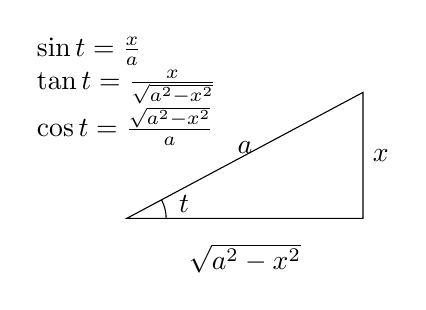
\begin{tikzpicture}[baseline=(char.base)]
        \node(char) at (0,0) {};
        \draw(0.5,-0.8) coordinate (A)--(3.5,-0.8) coordinate (B)--(3.5,0.8) coordinate (C)--cycle pic ["$t$",draw,angle radius=0.5cm,angle eccentricity=1.5] {angle = B--A--C};
        \node (cha) at ($(0.5,-1)!0.5!(3.5,-1)$) [below] {$\sqrt{a^2-x^2}$};
        \node (cha) at ($(3.5,-0.8)!0.5!(3.5,0.8)$) [right] {$x$};
        \node (cha) at ($(0.5,-1)!0.5!(3.5,0.8)$) [above] {$a$};
        \node (cha) at (0.5,0) [align=left,above] {$\sin t=\frac{x}{a}$\\$\tan t=\frac{x}{\sqrt{a^2-x^2}}$\\$\cos t=\frac{\sqrt{a^2-x^2}}{a}$};
    \end{tikzpicture}
\end{equation*}

\begin{examp}{求$\int \frac{1}{\sqrt{x^2-a^2}} \,\mathrm{d}x .$}
    \par \jie 首先考虑函数的定义域:$x^2-a^2> 0,x>a,x<-a$令$x=a\sec t,t \in (0,\frac{\pi}{2})\cup (\frac{\pi}{2},\pi),\int \frac{1}{\sqrt{x^2-a^2}} \,\mathrm{d}x =\int \frac{a\sec t\cdot\tan t}{\sqrt{a^2(\sec ^2t-1)}} \,\mathrm{d}t =\int \frac{\sec x\tan x}{\left\lvert \tan x\right\rvert } \,\mathrm{d}x ,$
    
    当$t \in (0,\frac{\pi}{2})$时,$\tan t>0,\tan t=\frac{\sqrt{x^2-a^2}}{a}.$故原式$=\ln \left\lvert \sec t+\tan t\right\rvert +C=\ln \left\lvert \frac{x}{a}+\frac{\sqrt{x^2-a^2}}{a}\right\rvert +C.$
    
    当$t \in (\frac{\pi}{2},\pi)$时,$\tan t<0,\tan t=-\frac{\sqrt{x^2-a^2}}{a}.$故原式$=-\ln \left\lvert \sec t+\tan t\right\rvert +C=-\ln \left\lvert \frac{x}{a}-\frac{\sqrt{x^2-a^2}}{a}\right\rvert +C=\ln \left\lvert \frac{x}{a}+\frac{\sqrt{x^2-a^2}}{a}\right\rvert +C.$

    故$\int \frac{1}{\sqrt{x^2-a^2}} \,\mathrm{d}x=\ln \left\lvert \frac{x}{a}+\frac{\sqrt{x^2-a^2}}{a}\right\rvert +C.$由于$a$为常数,所以可以进一步化简得$\int \frac{1}{\sqrt{x^2-a^2}} \,\mathrm{d}x=\ln \left\lvert x+\sqrt{x^2-a^2}\right\rvert +C.$
\end{examp}

\begin{examp}{求$\int_{3}^{+\infty} \frac{1}{\sqrt{x^2-2x}} \,\mathrm{d}x .$}
    \par \jie 首先配方$\int_{3}^{\infty} \frac{1}{\sqrt{(x-1)^2-1}} \,\mathrm{d}x $定积分使用三角换元最重要的就是观察它的定义域,因为求原函数要考虑到所有可能的$x$,但求定积分主要考虑给定的区间.由于积分下限是$(3,+\infty),$此时$(x-1)^2-1>0$恒成立,故可令$x-1=\sec t,t \in (0,\frac{\pi}{2}),$不用再考虑$t \in (\frac{\pi}{2},\pi)$的情况.
\end{examp}

\begin{examp}{求$\int \frac{\arcsin\sqrt{x}}{\sqrt{x}} \,\mathrm{d}x .$}
    \par \jie 令$t=\arcsin\sqrt{x},\because \sqrt{x}\geqslant 0\therefore \arcsin\sqrt{x} \in (0,\frac{\pi}{2})\therefore \cos t>0.$其实此处令$\sqrt{x}=t$更优.
\end{examp}

使用分部积分法时取$u$为易于积分的式子,注:$e^x,\cos x,\sin x$,取$v$为易于微分的式子,如高次多项式$P_n(x),\ln x,\arcsin x,\arccos x,\arctan x.$

\begin{equation*}
    \int \tikzmarknode[fill=Blue!20]{b1}{u}v \,\mathrm{d}\tikzmarknode[fill=Blue!20]{b2}{x} \implies \int v \,\mathrm{d}u =u\cdot v-\int u \,\mathrm{d}v =u\cdot v-\int u\cdot \tikzmarknode[fill=Blue!20]{b3}{v'} \,\mathrm{d}x .
    \tikz[remember picture,overlay]{\draw[->,Vintage_4,bend left=60] (b1.north) to (b2.north) node[above,yshift=0.6em](){e.g.$\,e^x,\cos x,\sin x$};\node[above,yshift=0.6em,Vintage_4] at (b3){e.g.$\,P_n(x),\ln x,\arcsin x,\arccos x,\arctan x$};}
\end{equation*}

当$v$是高次多项式时,可以有分部积分的推广方法:
\begin{equation*}
    \int u^{(n+1)}v \,\mathrm{d}x = u^{(n)}v -\int u^{(n)} \,\mathrm{d}v .
\end{equation*}
可以画表解决:
\begin{figure}[htp]
\centering
    \begin{tikzpicture}
        \matrix
        {
        \node (1){对$u$积分}; & \node (2){$u^{n+1}$}; & \node (3){$u^n$}; & \node (4){$u^{n-1}$}; & \node (5){$\dots$}; & \node (6){$u$}; \\
        \node (9){对$v$微分}; & \node (10){$v$}; & \node (11){$v'$}; & \node (12){$v''$}; & \node (13){$\dots$}; & \node (14){$v^{(n)}=0$}; \\
        };
        \draw[->,Vintage_4,thick](10.center)--(3.center) node [below,left]{$+$} (11.center)--(4.center) node [below,left]{$-$} (12.center)--(5.center) node [below,left]{$+$} (13.center)--(6.center) node [below,left]{$-$} ;
    \end{tikzpicture}
\caption{高次多项式时的分部积分法}
\end{figure}

\begin{examp}{$\displaystyle \int x\frac{\cos x}{\sin ^3x} \,\mathrm{d}x $}
    \par \jie $\int x\frac{1}{\sin ^3x} \,\mathrm{d}\sin x=\int x\frac{1}{-2} \,\mathrm{d}\sin ^{-2}x =-\frac{1}{2}\int x \,\mathrm{d}\sin ^{-2}x \\
    =-\frac{1}{2}\left( x\sin ^{-2}x-\int \sin ^{-2}x \,\mathrm{d}x \right)=-\frac{1}{2}\left( x\sin ^{-2}x-\int \csc ^2x \,\mathrm{d}x \right)\\
    =-\frac{1}{2}\left( x\sin^{-2}x+\cot x \right)+C.$
\end{examp}

一些复杂的式子可以多次使用分部积分法,利用对称性解出原式.对称性是说化简过程中等式左边的式子出现在了右边,常见的方法是分部积分或定积分换元.
\begin{examp}{$\displaystyle \int_{-\frac{\pi}{4}}^{\frac{\pi}{4}} e^{\frac{x}{2}}\frac{\cos x-\sin x}{\sqrt{\cos x}} \,\mathrm{d}x $}
    \par \jie $\int_{-\frac{\pi}{4}}^{\frac{\pi}{4}} \mathrm{e}^{\frac{x}{2}}\frac{\cos x}{\sqrt{\cos x}} \,\mathrm{d}x -\int_{-\frac{\pi}{4}}^{\frac{\pi}{4}} \mathrm{e}^{\frac{x}{2}}\frac{\sin x}{\sqrt{\cos x}} \,\mathrm{d}x\\
    =\int_{-\frac{\pi}{4}}^{\frac{\pi}{4}} \mathrm{e}^{\frac{x}{2}}\sqrt{\cos x} \,\mathrm{d}x+\int_{-\frac{\pi}{4}}^{\frac{\pi}{4}} \mathrm{e}^{\frac{x}{2}}\frac{1}{\sqrt{\cos x}} \,\mathrm{d}\cos x \\
    =\int_{-\frac{\pi}{4}}^{\frac{\pi}{4}} \mathrm{e}^{\frac{x}{2}}\sqrt{\cos x} \,\mathrm{d}x+\int_{-\frac{\pi}{4}}^{\frac{\pi}{4}} \mathrm{e}^{\frac{x}{2}} \,\mathrm{d}2\sqrt{\cos x}\\
    =\int_{-\frac{\pi}{4}}^{\frac{\pi}{4}} \mathrm{e}^{\frac{x}{2}}\sqrt{\cos x} \,\mathrm{d}x+2\left( \mathrm{e}^{\frac{x}{2}}\sqrt{\cos x}\vert ^{\frac{\pi}{4}}_{-\frac{\pi}{4}}-\frac{1}{2}\int_{-\frac{\pi}{4}}^{\frac{\pi}{4}} \mathrm{e}^{\frac{x}{2}}\frac{\cos x}{\sqrt{\cos x}} \,\mathrm{d}x \right)=2\mathrm{e}^{\frac{x}{2}}\sqrt{\cos x}\vert ^{\frac{\pi}{4}}_{-\frac{\pi}{4}} \\
    =2^{\frac{3}{4}}(\mathrm{e}^{\frac{\pi}{8}}-\mathrm{e}^{-\frac{\pi}{8}}).$
\end{examp}

\begin{examp}{$\displaystyle \int_{0}^{\frac{\pi}{2}} \frac{\sin t}{\sin t+\cos t} \,\mathrm{d}t $}
    \par \jie 换元时是令$t=x-\frac{\pi}{2}$,还是$x=t-\frac{\pi}{2}$是根据函数特性来的,譬如对于$\cos (x-\frac{\pi}{2})=\cos t$,而$\sin (x-\frac{\pi}{2})=-\sin t$.这边若令$x=t-\frac{\pi}{2}$,分母处变成了$\sin t-\cos t$就无法利用对称性了.所以只能令$x=\frac{\pi}{2}-t$,$I=-\int_{\frac{\pi}{2}}^{0} \frac{\cos t}{\sin t+\cos t} \,\mathrm{d}t ,\implies 2I=1,I=\frac{1}{2}$.
\end{examp}

\begin{examp}{$\displaystyle \int_{0}^{2n} x(x-1)(x-2)\dots (x-2n) \,\mathrm{d}x .$}
    \par \jie 区间再现公式$I=\int_{0}^{2n}x(x-1)(x-2)\dots (x-2n)\mathrm{d}x=\int_{0}^{2n}(2n-x)(2n-1-x)\dots (-x)\mathrm{d}x=(-1)^{2n+1}\int_{0}^{2n}x(x-1)(x-2)\dots (x-2n)\mathrm{d}x=-I\\
    \implies 2I=0,I=0$
\end{examp}

\begin{examp}{计算反常积分:$\displaystyle \int_{0}^{\mathrm{e}} \ln x \,\mathrm{d}x $}
    \par \jie $x\ln x \vert^\mathrm{e}_0-\int_{0}^{\mathrm{e}} x \,\mathrm{d}\ln x =\lim_{\varepsilon \to 0^+}x\ln x\vert ^\mathrm{e}_\varepsilon -x\vert^\mathrm{e}_0=\mathrm{e}-\lim_{\varepsilon \to 0^+}\varepsilon\ln \varepsilon-\mathrm{e}\\
    =-\lim_{\varepsilon \to 0^+}\frac{\ln \varepsilon}{\frac{1}{\varepsilon}}=\lim_{\varepsilon \to 0^+}-\varepsilon=0.$
\end{examp}
\begin{examp}{计算Euler积分:$\displaystyle \int_{0}^{\frac{\pi}{2}} \ln \sin x \,\mathrm{d}x $}
    \par \jie 法一,区间再现公式:$I=\int_{0}^{\frac{\pi}{2}}  \,\mathrm{d}x =\int_{0}^{\frac{\pi}{2}} \ln \sin (\frac{\pi}{2}+0-x) \,\mathrm{d}x =\int_{0}^{\frac{\pi}{2}} \ln \cos x \,\mathrm{d}x \\
    2I=\int_{0}^{\frac{\pi}{2}} \ln \sin x \,\mathrm{d}x +\int_{0}^{\frac{\pi}{2}} \ln \cos x \,\mathrm{d}x \\
    =\int_{0}^{\frac{\pi}{2}} \ln \sin x\cos x \,\mathrm{d}x =\int_{0}^{\frac{\pi}{2}} \ln \frac{1}{2}\sin 2x \,\mathrm{d}x =\int_{0}^{\frac{\pi}{2}} \left( \ln \frac{1}{2} +\ln \sin 2x  \right)\,\mathrm{d}x \\
    =\ln \frac{1}{2}\cdot x\vert ^\frac{\pi}{2}_0 +\int_{0}^{\frac{\pi}{2}} \ln \sin 2x \,\mathrm{d}x \xlongequal{t=2x} -\frac{\pi}{2}\ln 2 +\int_{0}^{\pi} \ln \sin t \,\mathrm{d}\frac{1}{2}t =-\frac{\pi}{2}\ln 2 +\frac{1}{2}\int_{0}^{\pi} \ln \sin t \,\mathrm{d}t \\
    \xlongequal{t-\frac{\pi}{2}=\mu} -\frac{\pi}{2}\ln 2 +\frac{1}{2}\int_{-\frac{\pi}{2}}^{\frac{\pi}{2}} \ln \cos \mu \,\mathrm{d}\mu=-\frac{\pi}{2}\ln 2 +\int_{0}^{\frac{\pi}{2}} \ln \cos \mu \,\mathrm{d}\mu=-\frac{\pi}{2}\ln 2 +I\\
    I=-\frac{\pi}{2}\ln 2.$

    法二,换元,使之能够使用二倍角公式:令$x=2t,\int_{0}^{\frac{\pi}{2}} \ln \sin x \,\mathrm{d}x =\int_{0}^{\frac{\pi}{4}} \ln \sin 2t \,\mathrm{d}t =2 \int_{0}^{\frac{\pi}{4}} \ln \left( 2\sin t\cos t \right) \,\mathrm{d}t =2\int_{0}^{\frac{\pi}{4}} \ln 2 \,\mathrm{d}t+2\int_{0}^{\frac{\pi}{4}} \ln \sin t \,\mathrm{d}t+2\int_{0}^{\frac{\pi}{4}} \ln \cos t \,\mathrm{d}t.$
    
    对$2\int_{0}^{\frac{\pi}{4}} \ln \cos t \,\mathrm{d}t$换元,令$\frac{\pi}{2}-t=\mu,2\int_{0}^{\frac{\pi}{4}} \ln \cos t \,\mathrm{d}t=-2\int_{\frac{\pi}{2}}^{\frac{\pi}{4}} \sin \mu \,\mathrm{d}\mu =2\int_{\frac{\pi}{4}}^{\frac{\pi}{2}} \sin \mu \,\mathrm{d}\mu .$
    
    代回原式:$I=2\int_{0}^{\frac{\pi}{4}} \ln 2 \,\mathrm{d}t+2\int_{0}^{\frac{\pi}{4}} \ln \sin t \,\mathrm{d}t+2\int_{\frac{\pi}{4}}^{\frac{\pi}{2}} \ln \sin t \,\mathrm{d}t.=\frac{\pi}{2}\ln 2+2\int_{0}^{\frac{\pi}{2}} \ln \sin t \,\mathrm{d}t=\frac{\pi}{2}\ln 2+2I \implies I=\int_{0}^{\frac{\pi}{2}} \ln \sin x \,\mathrm{d}x =-\frac{\pi}{2}\ln 2$
\end{examp}

\begin{examp}{求定积分$I=\int_{0}^{2} \sqrt{\left(1-\frac{1}{4}x^2\right) ^3}\,\mathrm{d}x $}
    
    \jie 三角换元+华里士公式

    令$x=2\sin t$,则$I=\int_{0}^{2} \sqrt{\left(1-\frac{1}{4}x^2\right) ^3}\,\mathrm{d}x =2 \int_{0}^{\frac{\pi}{2}} \cos^4 t \,\mathrm{d}t =\frac{3 \pi}{8}$
\end{examp}

\begin{examp}{求定积分$I=\int_{0}^{\pi} \frac{\left\lvert x \sin x \cos x\right\rvert }{1+\cos^2x} \,\mathrm{d}x $}
    
    \jie 本题体现了定积分计算的多种技巧.
    
    首先用区间再现公式消去分子上的$x$:
    
    $I=\int_{0}^{\pi} \frac{x\left\lvert  \sin x \cos x\right\rvert }{1+\cos^2x} \,\mathrm{d}x =\int_{0}^{\pi} \frac{(\pi-x)\left\lvert  \sin x \cos x\right\rvert }{1+\cos^2x} \,\mathrm{d}x \implies 2I=\int_{0}^{\pi} \frac{\pi\left\lvert  \sin x \cos x\right\rvert }{1+\cos^2x} \,\mathrm{d}x $

    其次我们观察到变量主要是三角函数,这代表着原函数可能具有周期性,周期$T=\pi$,故我们要用周期性把区间调整到一个关于原点对称的区间:
    
    $I=\frac{1}{2}\int_{0}^{\pi} \frac{\pi\left\lvert  \sin x \cos x\right\rvert }{1+\cos^2x} \,\mathrm{d}x =\frac{\pi}{2}\int_{-\frac{\pi}{2}}^{\frac{\pi}{2}} \frac{\left\lvert  \sin x \cos x\right\rvert }{1+\cos^2x} \,\mathrm{d}x $

    此时观察原函数的奇偶性,发现原函数是偶函数,故得:

    $I=\pi\int_{0}^{\frac{\pi}{2}} \frac{\left\lvert  \sin x \cos x\right\rvert }{1+\cos^2x} \,\mathrm{d}x $

    这时候发现分子绝对值符号内必然为正,故绝对值也去掉了:

    $I=-\frac{\pi}{2}\int_{0}^{\frac{\pi}{2}} \frac{1}{1+\cos^2x} \,\mathrm{d}\cos^2x =\frac{\pi}{2}\ln 2$
\end{examp}

常用的几种积分方法:
\begin{align*}
    \enulabel{1.}&\int \frac{1}{(x^2+4)^2} \,\mathrm{d}x &
    \enulabel{2.}&\int \frac{1}{x^2+4} \,\mathrm{d}x &
    \enulabel{3.}&\int \frac{1}{x^2-1} \,\mathrm{d}x &
    \enulabel{4.}&\int x\sqrt{1-9x^2} \,\mathrm{d}x \\
    \enulabel{5.}&\int \frac{(x-1)^2}{\sqrt[3]{x}} \,\mathrm{d}x &
    \enulabel{6.}&\int \frac{\sqrt{x}}{\sqrt{4-x^3}} \,\mathrm{d}x &
    \enulabel{7.}&\int \frac{1}{\sqrt{1-x}} \,\mathrm{d}x &
    \enulabel{8.}&\int \frac{x^2-5}{x^2+1} \,\mathrm{d}x \\
    \enulabel{9.}&\int \sec x \,\mathrm{d}x &
    \enulabel{10.}&\int \cos ^2x \,\mathrm{d}x &
    \enulabel{11.}&\int \cos ^3x \,\mathrm{d}x &
    \enulabel{12.}&\int \sin ^4x \,\mathrm{d}x \\
    \enulabel{13.}&\int \frac{1}{1+\cos x} \,\mathrm{d}x &
    \enulabel{14.}&\int \frac{1}{1+\sqrt{x}} \,\mathrm{d}x &
    \enulabel{15.}&\int \frac{\sqrt{x}}{1-x} \,\mathrm{d}x &
    \enulabel{16.}&\int \frac{1}{\cos ^3\theta} \,\mathrm{d}\theta \\
    \enulabel{17.}&\int x^2\sqrt{1-x^2} \,\mathrm{d}x &
    \enulabel{18.}&\int \frac{x}{\sqrt{x+1}} \,\mathrm{d}x &
    \enulabel{19.}&\int x^2\sqrt{6x-x^2} \,\mathrm{d}x &
    \enulabel{20.}&\int \frac{\sqrt{x^2-9}}{x^4} \,\mathrm{d}x \\
    \enulabel{21.}&\int \frac{1}{x\sqrt{x^4+1}} \,\mathrm{d}x &
    \enulabel{22.}&\int \frac{1}{\sqrt{x^2-a^2}} \,\mathrm{d}x &
    \enulabel{23.}&\int \frac{1}{\sqrt{x^2+a^2}} \,\mathrm{d}x &
    \enulabel{24.}&\int \sqrt{a^2-x^2} \,\mathrm{d}x \\
    \enulabel{25.}&\int \frac{1}{x^2+x} \,\mathrm{d}x  &
    \enulabel{26.}&\int \frac{1}{\mathrm{e}^{x+1}+\mathrm{e}^{3-x}} \,\mathrm{d}x &
    \enulabel{27.}&\int \frac{1}{\mathrm{e}^{2x}+1} \,\mathrm{d}x &
    \enulabel{28.}&\int \frac{1}{\mathrm{e} ^x+1} \,\mathrm{d}x 
\end{align*}

设有两个多项式:$P_n(x),Q_m(x),$其中$n,m$分别是这两个多项式的最高次幂,若有$\dfrac{P_n(x)}{Q_m(x)}$,当$n\geqslant m$时,总是可以拆成一个多项式的和,容易积分,如题3,5,8,25,27.当$n<m$可以考虑使用倒代换的方法,令$t=\frac{1}{x}.$如题18,20.但如果$P_n(x),Q_m(x)$是根式,直接换元更加方便.题4,6,7,11,26,27,28用凑微分法;题7,14,15,16,18用换元法;题1,17,19,21,22,23,24用三角换元;题10,11,12,13用三角函数的降幂公式.

题1令$x=2\tan t$.题2$\int \frac{1}{x^2+4} \,\mathrm{d}x=\int \frac{1}{4\left[ \left( \frac{x}{2} \right)^2+1 \right]} \,\mathrm{d}x$.题3用有理函数的积分方法,将$\int \frac{1}{x^2-1} \,\mathrm{d}x $化为$\frac{1}{2}\int \frac{1}{x-1}-\frac{1}{x+1} \,\mathrm{d}x ,$然后分别积分.题4凑$\frac{1}{2}\int \sqrt{1-9x^2} \,\mathrm{d}x^2 $.

题5拆为$\int \left(x^{\frac{5}{3}}-2x^{\frac{2}{3}}+x^{-\frac{1}{3}}\right) \,\mathrm{d}x .$题6凑为$\frac{2}{3}\int \frac{\mathrm{d}x^{\frac{3}{2}}}{\sqrt{4-x^3}} =\frac{1}{3}\int \frac{\mathrm{d}x^{\frac{3}{2}}}{\sqrt{1-\left(\frac{x^{3/2}}{2}\right) ^2}} =\frac{1}{3}\arctan x^{\frac{3}{2}}+C$.题7凑为$-\int \frac{\mathrm{d}(1-x)}{\sqrt{1-x}} =-2\sqrt{1-x}.$题8凑为$\int 1-\frac{6}{x^2+1} \,\mathrm{d}x .$

题9化为$\int \frac{1}{\cos x} \,\mathrm{d}x =\int \frac{\cos x}{\cos ^2x} \,\mathrm{d}x=\int \frac{\mathrm{d}\sin x}{1-\sin ^2x} .$题10化为$\int \frac{1+\cos 2x}{2} \,\mathrm{d}x .$题11化为$\int (1-\sin ^2x) \,\mathrm{d}\sin x .$题12化为$\int \left(\frac{1-\cos 2x}{2}\right) ^2 \,\mathrm{d}x .$

题13化为$\int \frac{1}{2\cos ^2\frac{x}{2}} \,\mathrm{d}x =\int \sec ^2\frac{x}{2} \,\mathrm{d}\frac{x}{2} .$题14换元,令$\sqrt{x}=t,\int \frac{1}{1+\sqrt{x}} \,\mathrm{d}x =\int \frac{2t}{1+t} \,\mathrm{d}t .$题15换元,令$\sqrt{x}=t,\int \frac{\sqrt{x}}{1-x} \,\mathrm{d}x =2\int \frac{t^2}{1-t^2} \,\mathrm{d}t =-2\int \left( 1-\frac{1}{1-t^2} \right) \,\mathrm{d}t .$题16有两种方法,$\int \frac{1}{\cos ^3\theta} \,\mathrm{d}\theta=\int \frac{1}{\cos ^4\theta} \,\mathrm{d}\sin \theta =\int \frac{1}{(1-\sin ^2\theta)^2} \,\mathrm{d}\sin \theta .$然后用换元,令$t=\sin \theta$,此处就可以参考有理函数的积分方法,$\int \frac{1}{(1-t^2)^2} \,\mathrm{d}t =\frac{1}{4}\left(\left(\frac{1}{1-t}\right) ^2+\ln \frac{1+t}{1-t}-\left(\frac{1}{1+t}\right) ^2\right) +C$.第二种方法$\int \frac{1}{\cos ^3\theta} \,\mathrm{d}\theta=\int \frac{\sin ^2\theta+\cos ^2\theta}{\cos ^3\theta} \,\mathrm{d}x =\int \frac{\sin^2 \theta}{\cos ^3\theta} \,\mathrm{d}\theta+\int \frac{1}{\cos\theta} \,\mathrm{d}\theta =-\int \frac{\sin \theta}{\cos ^3\theta} \,\mathrm{d}\cos \theta +\ln \left\lvert \sec\theta+\tan \theta\right\rvert +C=\frac{1}{2}\int \sin \theta \,\mathrm{d}\frac{1}{\cos^2 \theta} +\ln \left\lvert \sec\theta+\tan \theta\right\rvert +C=\frac{1}{2}\frac{\sin \theta}{\cos^2\theta}-\frac{1}{2}\int \frac{1}{\cos ^2\theta} \,\mathrm{d}\sin \theta +\ln \left\lvert \sec\theta+\tan \theta\right\rvert +C =\frac{1}{2}\frac{\sin \theta}{\cos^2\theta}+\frac{1}{2}\int \frac{1}{\sin ^2\theta-1} \,\mathrm{d}\sin \theta +\ln \left\lvert \sec\theta+\tan \theta\right\rvert +C =\frac{1}{2}\frac{\sin \theta}{\cos^2\theta}+\frac{1}{4}\ln \left\lvert \frac{\sin \theta-1}{\sin \theta+1}\right\rvert  +\ln \left\lvert \sec\theta+\tan \theta\right\rvert +C $

题17用三角换元,令$x=\sin t,\int x^2\sqrt{1-x^2} \,\mathrm{d}x =\int \sin ^2t\cos t\cdot\cos t \,\mathrm{d}t .$题18换元,令$\sqrt{x+1}=t,\int \frac{x}{\sqrt{x+1}} \,\mathrm{d}x=2 \int (t^2-1) \,\mathrm{d}t .$题19要先在根号内配方$\int x^2\sqrt{9-(x-3)^2} \,\mathrm{d}x $,然后用三角换元,令$x-3=3\sin t.$题20换元,令$x=\frac{1}{t},\int \frac{\sqrt{x^2-9}}{x^4} \,\mathrm{d}x=\int \sqrt{(1-9t^2)} \left\lvert t\right\rvert \,\mathrm{d}t .$

题21有多种方法,可以使用倒代换,分母有$\sqrt{x^4+1}$也可以采用三角换元,但此类题目有一个固定的解法$\int \frac{1}{x\sqrt{x^4+1}} \,\mathrm{d}x =\int \frac{1}{x\cdot x^2\sqrt{1+\frac{1}{x^4}}} \,\mathrm{d}x =-\frac{1}{2}\int \frac{1}{\sqrt{1+\frac{1}{x^4}}} \,\mathrm{d}x^{-2} =-\frac{1}{2}\int \frac{1}{\sqrt{1+(\frac{1}{x^2})^2}} \,\mathrm{d}\frac{1}{x^2} =-\frac{1}{2}\ln \left\lvert \frac{1}{x^2}+\sqrt{1+\frac{1}{x^4}}\right\rvert+C$

题25用有理函数的积分方法,$\int \frac{1}{x(x+1)} \,\mathrm{d}x =\int \frac{1}{x}-\frac{1}{x+1} \,\mathrm{d}x .$题26凑微分$\int \frac{\mathrm{e}^{x-3}}{\mathrm{e}^{2(x-1)}+1} \,\mathrm{d}x =\frac{1}{\mathrm{e}^2}\int \frac{\mathrm{e}^{x-1}}{\mathrm{e}^{2(x-1)}+1} \,\mathrm{d}x =\frac{1}{\mathrm{e}^2}\int \frac{\mathrm{d}\mathrm{e}^{(x-1)}}{\mathrm{e}^{2(x-1)}+1} .$题27应与题16,28对照起来看$\int \frac{1+\mathrm{e}^{2x}-\mathrm{e}^{2x}}{\mathrm{e}^{2x}+1} \,\mathrm{d}x =\int \left(1-\frac{\mathrm{e}^{2x}}{\mathrm{e}^{2x}+1}\right)  \,\mathrm{d}x =x-\frac{1}{2}\int \frac{\mathrm{d}(\mathrm{e}^{2x}+1)}{\mathrm{e}^{2x}+1} .$如果题27不用这个方法,而采用题1所提示的方法也是可以的,但是复杂程度大大提高,而且难算,所以应记住这一凑微分的特殊方法.此处换元还应注意定义域:$e^x=\tan t,t \in (0,\frac{\pi}{2}),x=\ln \tan t,t=\arctan e^x,\int \frac{1}{\mathrm{e}^{2x}+1} \,\mathrm{d}x =\int \frac{\frac{1}{\tan t}\cdot\sec ^2t}{\tan ^2t+1} \,\mathrm{d}t =\int \cot t \,\mathrm{d}t =\ln \left\lvert \sin t\right\rvert +C,\because t \in (0,\frac{\pi}{2})\therefore \sin t=\frac{\mathrm{e}^x}{\sqrt{\mathrm{e}^{2x}+1}}>0 \therefore \ln \left\lvert \sin t\right\rvert +C=\frac{1}{2}\ln \frac{\mathrm{e}^{2x}}{\mathrm{e}^{2x}+1}+C=\frac{1}{2}\left( \ln \mathrm{e}^{2x}-\ln (\mathrm{e}^{2x}+1) \right)+C=\frac{1}{2}\left( 2x-\ln (\mathrm{e}^{2x}+1) \right)+C.$题28$\int \frac{1}{\mathrm{e} ^x+1} \,\mathrm{d}x=\int \frac{\mathrm{e} ^{-x}}{1+\mathrm{e} ^{-x}} \,\mathrm{d}x =-\int \frac{1}{1+\mathrm{e} ^{-x}} \,\mathrm{d}\mathrm{e} ^{-x} $

\begin{definition}[有理函数]
设有两个多项式:
    \begin{align*}
        P(x)&=a_0x^n+a_1x^{n-1}+\cdots+a_{n-1}x+a_n,\\
        Q(x)&=b_0x^m+b_1x^{m-1}+\cdots+b_{m-1}x+b_m.
    \end{align*}

其中$m,n$都是非负整数,$a_0,\dots,a_n,b_0,\dots,b_n$都是实数,且$a_0\neq 0,b_0\neq 0.$则我们称函数$\frac{P(x)}{Q(x)}$为有理函数.若$n\geqslant m,$则可以把这个函数拆成一个多项式和一个真分式的和.任一真分式又可以拆成若干个简单的分式之和,这些简单的分式只有如下四种形式:
    \begin{align*}
        &\frac{A}{x-a}&
        &\frac{A}{(x-a)^2}\\
        &\frac{Ax+B}{x^2+px+q}&
        &\frac{Ax+B}{(x^2+px+q)^2}
    \end{align*}
其中$p^2-4q<0.$
\end{definition}
需要注意的是,如果后两种分式中的分母不满足$p^2-4q<0,$就一定可以继续拆分化为前面两种.使用待定系数法有可能出现无解的情况,这时候就要检查是否分母还可以再拆.

\txe{注:}$\frac{1}{(\mu^2-1)(\mu+1)},$若设成$\frac{A\mu+B}{\mu^2-1}+\frac{C}{\mu+1}$无解,须设成$\frac{A}{(\mu+1)^2}+\frac{B}{\mu-1}$.

当分式拆成如上四种形式后,前两种形式用凑微分法易于积分,后两种形式由于分母已经不可再拆,要在分子上凑出分母的微分,由于分子的幂数总是比分母低,所以分子上最后会剩下一个常数,这时候对该项积分只要把分母凑成完全平方式即可.

形式三凑出的分母只有$\int \frac{1}{\varphi ^2(x)\pm a^2} \,\mathrm{d}\varphi (x) $两种情形,对于$\int \frac{1}{\varphi ^2(x)+ a^2} \,\mathrm{d}\varphi (x) =\int \frac{1}{a^2\left[(\frac{\varphi (x)}{a})^2+1\right] } \,\mathrm{d}\varphi (x) =\frac{1}{a^2}\arctan \varphi (x) +C$.对于$\int \frac{1}{\varphi ^2(x)- a^2} \,\mathrm{d}\varphi (x) =\int \frac{1}{(\varphi (x)+a)(\varphi (x)-a)} \,\mathrm{d}\varphi (x) =\frac{1}{2a}\int \left(\frac{1}{\varphi (x)-a}-\frac{1}{\varphi (x)+a}\right)  \,\mathrm{d}\varphi (x) =\frac{1}{2a}\ln \left\lvert \frac{\varphi (x)-a}{\varphi (x)+a}\right\rvert +C$.

形式四凑出的分母只有$\int \frac{1}{(\varphi ^2(x)\pm a^2)^2} \,\mathrm{d}\varphi (x) $两种情形,对于$\int \frac{1}{(\varphi ^2(x)+ a^2)^2} \,\mathrm{d}\varphi (x)$然后可以参考“常用的几种积分方法”的第一题,用三角换元,令$\varphi (x) =a\tan t$即可.对于$\int \frac{1}{(\varphi ^2(x)- a^2)^2} \,\mathrm{d}\varphi (x)=\frac{1}{4a^2}\int \left(\frac{1}{\varphi (x)-a}-\frac{1}{\varphi (x)+a}\right) ^2 \,\mathrm{d}\varphi (x) \\
=\frac{1}{4a^2}\int \left(\left(\frac{1}{\varphi (x)-a}\right) ^2-2\frac{1}{\varphi (x)-a}\frac{1}{\varphi (x)+a}+\left(\frac{1}{\varphi (x)+a}\right) ^2\right) \,\mathrm{d}\varphi (x) \\
=\frac{1}{4a^2}\left(-\frac{1}{\varphi (x)-a}-\frac{1}{a}\ln\left\lvert \frac{\varphi (x)-a}{\varphi (x)+a}\right\rvert -\frac{1}{\varphi (x)+a}\right) +C$

\begin{examp}{拆分有理函数的例子:
\begin{align*}
    \enulabel{1.}&\int \frac{\mathrm{d}x}{x(x-1)^2}&
    \enulabel{2.}&\int \frac{2x+4}{(x-1)(x^2+1)} \, \mathrm{d}x\\
    \enulabel{3.}&\int \frac{2x+1}{(x^2-6x+10)^2} \, \mathrm{d}x&
    \enulabel{4.}&\int \frac{5x+1}{\sqrt{4x^2-4x+3}} \, \mathrm{d}x
\end{align*}}

\jie 题1.设$\frac{1}{x(x-1)^2}=\frac{A}{x}+\frac{B}{(x-1)^2} \implies A(x-1)^2+Bx=1$,特殊值法代入$x=0,x=1,\implies A=1,B=1,\int \left(\frac{1}{x}+\frac{1}{(x-1)^2} \right)  \,\mathrm{d}x$

题2.设$\frac{2x+4}{(x-1)(x^2+1)}=\frac{A}{x-1}+\frac{Bx+C}{(x^2+1)} \implies A(x^2+1)+(Bx+C)(x-1)=2x+4$,特殊值法代入$x=0,x=1,\implies A=3,B=-3,C=-1$

题3.$\int \frac{2x+1}{(x^2-6x+10)^2} \,\mathrm{d}x =\int \frac{(2x-6)+7}{(x^2-6x+10)^2} \,\mathrm{d}x \\
=-(x^2-6x+10)^{-1}+7\int \frac{1}{\left[(x-3)^2+9\right] ^2} \,\mathrm{d}x $.令$x-3=\tan t,t \in \left(-\frac{\pi}{2},\frac{\pi}{2}\right) $即可.

题4.虽然不是有理函数,但是处理的方法类似:

$\int \frac{5x+1}{\sqrt{4x^2-4x+3}} \, \mathrm{d}x\\
=\int \frac{\frac{5}{8}(8x-4)+\frac{7}{2}}{\sqrt{4x^2-4x+3}} \,\mathrm{d}x =\frac{5}{4}\sqrt{4x^2-4x+3}+\frac{7}{2}\cdot\frac{1}{2}\int \frac{1}{\sqrt{(2x-1)^2+2}} \,\mathrm{d}(2x-1) \\
=\frac{5}{4}\sqrt{4x^2-4x+3}+\frac{7}{4}\ln\left\lvert  2x-1+\sqrt{4x^2-4x+3}\right\rvert +C$

最后一步直接套用公式.
\end{examp}

\subsubsection{定积分的精确定义(黎曼积分)}
\begin{equation*}
    \int_{a}^{b} f(x) \,\mathrm{d}x =\lim_{n \to \infty}\sum^{n}_{i=1}f\left(a+\frac{b-a}{n}i \right)\frac{b-a}{n}.
\end{equation*}

当求数列极限夹逼定理失效时,我们可以考虑将离散求和化为积分的形式.一般我们做题时把$b$看作$1$,$a$看作$0$,得$a+\frac{b-a}{n}i =\frac{i}{n}$,再将所求函数提出$\frac{1}{n}$,然后将函数的剩余部分化简成关于$\frac{1}{n}$的函数,然后将所求极限写成积分形式即可.

\begin{figure}[htp]
\centering
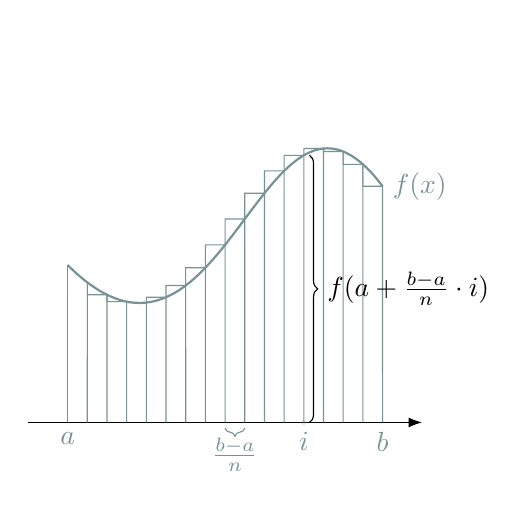
\begin{tikzpicture}
    \draw[->] (0,0) -- (5,0);
    \draw[thick,Vintage_4,domain=1:4,name path=func] (0.5,2) .. controls (2.5,0) and (3,5) .. (4.5,3) node[right] {$f(x)$};
    \draw[Vintage_4] (0.5,0) node[below] {$a$} -- (0.5,2) (4.5,0) node[below] {$b$} -- (4.5,3);
    \foreach \min in {0.75,1,1.25,1.5,...,4.5}
        {\path[name path=agg] (\min,0) -- (\min,5);
        \path[name path=ag] (\min-0.25,0) -- (\min-0.25,5);
        \draw[Vintage_4,name intersections={of=agg and func, by=point},name intersections={of=ag and func, by=pnt},Vintage_4] let \p1 = (point), \p2=(pnt) in (\min,0) -- (point) -- (\x2,\y1) -- (pnt);
        }
    \path[name path=ab] (3.5,0) node[Vintage_4,below] {$i$} -- (3.5,5);
    \draw[name intersections={of=ab and func, by=point},decorate,decoration={brace,amplitude=3pt,mirror,raise=2pt}] (3.5,0) --node[xshift=5pt,right]{$f(a+\frac{b-a}{n}\cdot i)$} (point);
    \draw[Vintage_4,name intersections={of=ab and func, by=point},decorate,decoration={brace,amplitude=3pt,mirror,raise=2pt}] (2.5,0) --node[below,yshift=-2pt]{$\frac{b-a}{n}$} (2.75,0);
    \fill[Vintage_4,opacity=0.2](3.5,0) circle (1pt);
\end{tikzpicture}
\caption{黎曼积分的示意图}\label{riemann}
\end{figure}
\subsubsection{定积分的应用}
曲线$f(x)$和$x$轴围成的面积:
\begin{equation*}
    \int_{a}^{b} \left\lvert f(x)\right\rvert  \,\mathrm{d}x .
\end{equation*}

曲线$f(x),g(x)$之间的面积:
\begin{equation*}
    \int_{a}^{b} \left\lvert f(x)-g(x)\right\rvert  \,\mathrm{d}x .
\end{equation*}

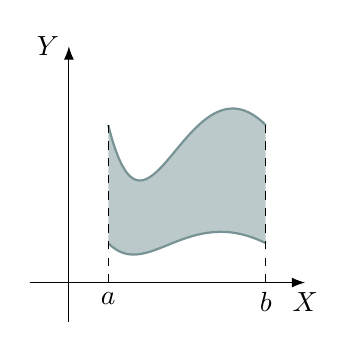
\begin{tikzpicture}
    \fill [fill = Vintage_4,fill opacity=0.5] (0.5,2) .. controls (1,0) and (1.5,3) .. (2.5,2) -- (2.5,0.5) -- (2.5,0.5) .. controls (1.5,1) and (1,0) .. (0.5,0.5) -- (0.5,2);
    \draw [->] (0,-0.5) -- (0,3) node[left] {$Y$};
    \draw [->] (-0.5,0) -- (3,0) node[below] {$X$};
    \draw [Vintage_4,thick] (0.5,2) .. controls (1,0) and (1.5,3) .. (2.5,2);
    \draw [Vintage_4,thick] (0.5,0.5) .. controls (1,0) and (1.5,1) .. (2.5,0.5);
    \draw [dashed] (0.5,0) node[below] {$a$} -- (0.5,2) (2.5,0) node[below] {$b$} -- (2.5,2); 
\end{tikzpicture}
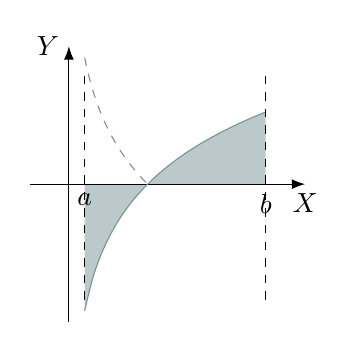
\begin{tikzpicture}
    \fill [fill = Vintage_4,fill opacity=0.5] [domain=0.2:1,smooth] plot(\x,{ln(\x)}) -- (0.2,0) -- cycle;
    \fill [fill = Vintage_4,fill opacity=0.5] [domain=1:2.5,smooth] plot(\x,{ln(\x)}) -- (2.5,0) -- cycle;
    \draw [->] (0,-1.75) -- (0,1.75) node[left] {$Y$};
    \draw [->] (-0.5,0) -- (3,0) node[below] {$X$};
    \draw [Vintage_4,domain=0.2:2.5,smooth] plot(\x,{ln(\x)});
    \draw [Vintage_4,domain=0.2:1,smooth,dashed] plot(\x,{-ln(\x)});
    \draw [dashed] (0.2,{0.35*(0.2-0.5)^2-1.5}) -- (0.2,0) node[below] {$a$} -- (0.2,{-0.35*(0.2-0.5)^2+1.5}) (2.5,{0.35*(0.2-0.5)^2-1.5}) -- (2.5,0) node[below] {$b$} -- (2.5,{-0.35*(0.2-0.5)^2+1.5}); 
\end{tikzpicture}
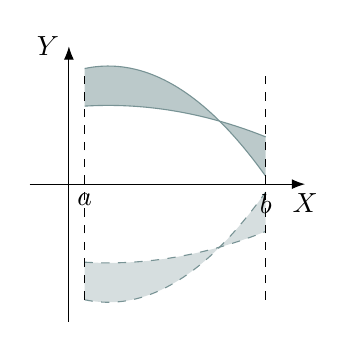
\begin{tikzpicture}
    \fill [fill = Vintage_4,fill opacity=0.5] [domain=0.2:2.5,smooth] plot(\x,{-0.35*(\x-0.5)^2+1.5}) -- (2.5,{-0.1*(2.5-0.5)^2+1}) [domain=2.5:0.2,smooth] -- plot(\x,{-0.1*(\x-0.5)^2+1}) -- cycle;
    \fill [fill = Vintage_4,fill opacity=0.3] [domain=0.2:2.5,smooth] plot(\x,{0.35*(\x-0.5)^2-1.5}) -- (2.5,{0.1*(2.5-0.5)^2-1}) [domain=2.5:0.2,smooth] -- plot(\x,{0.1*(\x-0.5)^2-1}) -- cycle;
    \draw [->] (0,-1.75) -- (0,1.75) node[left] {$Y$};
    \draw [->] (-0.5,0) -- (3,0) node[below] {$X$};
    \draw [Vintage_4,domain=0.2:2.5,smooth] plot(\x,{-0.35*(\x-0.5)^2+1.5});
    \draw [Vintage_4,domain=0.2:2.5,smooth] plot(\x,{-0.1*(\x-0.5)^2+1});
    \draw [Vintage_4,domain=0.2:2.5,smooth,dashed] plot(\x,{0.35*(\x-0.5)^2-1.5});
    \draw [Vintage_4,domain=0.2:2.5,smooth,dashed] plot(\x,{0.1*(\x-0.5)^2-1});
    \draw [dashed] (0.2,{0.35*(0.2-0.5)^2-1.5}) -- (0.2,0) node[below] {$a$} -- (0.2,{-0.35*(0.2-0.5)^2+1.5}) (2.5,{0.35*(0.2-0.5)^2-1.5}) -- (2.5,0) node[below] {$b$} -- (2.5,{-0.35*(0.2-0.5)^2+1.5}); 
\end{tikzpicture}

曲线$r=r(\theta)$与射线$\theta=\alpha,\theta=\beta$围成的面积:
\begin{equation*}
    \frac{1}{2}\int_{\alpha}^{\beta} r^2(\theta) \,\mathrm{d}\theta 
\end{equation*}

曲线$r=r_1(\theta),r=r_2(\theta)$与射线$\theta=\alpha,\theta=\beta$围成的面积:
\begin{equation*}
    \frac{1}{2}\int_{\alpha}^{\beta} \left\lvert r_1^2(\theta)-r_2^2(\theta)\right\rvert \,\mathrm{d}\theta 
\end{equation*}

\subsubsection{旋转体的体积}
连续曲线$y=f(x)$以及$x=a,x=b$和$x$轴绕$x$轴旋转而成的旋转体的体积为
\begin{equation*}
    V_x=\pi \int_{a}^{b} f^2(x) \,\mathrm{d}x .
\end{equation*}
连续曲线$x=\varphi (y)$以及$y=c,y=d$和$y$轴绕$y$轴旋转而成的旋转体的体积为
\begin{equation*}
    V_y=\pi \int_{c}^{d} \varphi ^2(y) \,\mathrm{d}y .
\end{equation*}
当$0\leqslant a<x<b$时也可以写成
\begin{equation*}
    V_y=2\pi \int_{a}^{b} x\left\lvert f(x)\right\rvert  \,\mathrm{d}x .
\end{equation*}
以上是曲线与$x$轴所围成的旋转体体积,如果是两条曲线围成的旋转体体积,只要将两个体积相减即可.对于一些比较复杂的曲线围成的旋转体体积,将曲线沿旋转轴折叠一下就比较容易看出.

\begin{examp}{求曲线$f(x)=\frac{1}{e}\sqrt{x}$与$g(x)=\ln \sqrt{x}$绕$x$轴一周所围成的旋转体的体积.}

    \jie 旋转体的图示如下:
\end{examp}

\begin{figure}[htp]
\centering
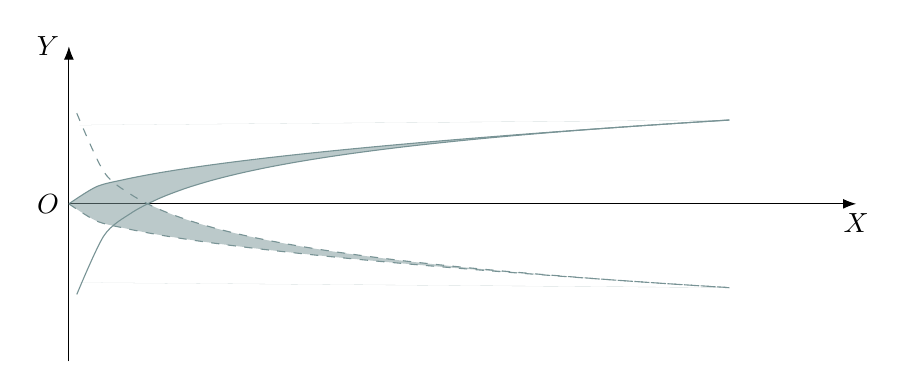
\begin{tikzpicture}
    \draw[->] (0,-2) -- (0,2) node[left] {$Y$};
    \draw[->] (0,0) -- (10,0) node[below] {$X$};
    \coordinate[label=left:$O$] (O) at (0,0);
    \draw [Vintage_4,domain=0:{e^2+1},smooth] plot(\x,{(1/e)*sqrt(\x)});
    \draw [Vintage_4,domain=0:{e^2+1},smooth,dashed] plot(\x,{-(1/e)*sqrt(\x)});
    \draw [Vintage_4,domain=0.1:{e^2+1},smooth] plot(\x,{ln(sqrt(\x))});
    \draw [Vintage_4,domain=0.1:{e^2+1},smooth,dashed] plot(\x,{-ln(sqrt(\x))});
    \fill [fill = Vintage_4,fill opacity=0.5] [domain=0:{e^2+1},smooth] plot(\x,{(1/e)*sqrt(\x)}) -- (1/e^2,1)[domain={e^2+1}:1,smooth] -- plot(\x,{ln(sqrt(\x))}) -- (0,0); 
    \fill [fill = Vintage_4,fill opacity=0.5] [domain=0:{e^2+1},smooth] plot(\x,{-(1/e)*sqrt(\x)}) -- (1/e^2,-1)[domain={e^2+1}:1,smooth] -- plot(\x,{-ln(sqrt(\x))}) -- (0,0); 
\end{tikzpicture}
\end{figure}

\subsubsection{二重积分}

轮换对称性:
\begin{enumerate}
    \item 若积分区域$D$交换$x,y$后没有发生变化(即积分区域关于$y=x$对称),那么有以下结论
    \begin{equation*}
        \iint_D f(x,y) \,\mathrm{d}\sigma=\iint_D f(y,x) \,\mathrm{d}\sigma.
    \end{equation*}
    因为对于任意积分区域内一点$(x_0,y_0)$,$(y_0,x_0)$也在区域内.
    \item 若积分区域$D$关于$y=x$对称的同时,被积函数$f(x,y)$交换$x,y$后还是原来的函数,那么积分区域两个对称的部分$D_1,D_2$积分值相等,即
    \begin{equation*}
        \iint_D f(x,y) \,\mathrm{d}\sigma=2\iint_{D_1} f(y,x) \,\mathrm{d}\sigma=2\iint_{D_2} f(y,x) \,\mathrm{d}\sigma
    \end{equation*}
\end{enumerate}


极坐标与直角坐标的相互转换:
$\begin{dcases}
    x=r\cos \theta,\\
    y=r\sin \theta,\\
    r^2=x^2+y^2 \implies r=\sqrt{x^2+y^2}.
\end{dcases}$

解决二重积分时先观察积分区域是否部分或全部关于$x,y$轴对称,如果是,可以利用对称性来简化运算.如果积分区域在平移后能产生对称性,不妨用换元法求这个二重积分.
\begin{figure}[htp]
\centering
    \begin{tikzpicture}
        \draw[->] (-2,0) -- (2,0) node[below] {$Y$};
        \draw[->] (0,-2) -- (0,2) node[left] {$X$};
        \draw (1,-1) -- (1,1) (-1,-1) -- (1,-1);
        \draw [domain=-1:1,smooth] plot(\x,\x);
        \draw [domain=0:1,smooth,dashed] plot(\x,-\x);
    \end{tikzpicture}
    \caption{二重积分的积分区域既关于$x$轴又关于$y$轴对称}
\end{figure}

\begin{examp}{计算泊松积分$\displaystyle \int_{-\infty}^{\infty} e^{-x^2} \,\mathrm{d}x $}
    \par \jie 令$I=\int_{-\infty}^{+\infty} e^{-x^2} \,\mathrm{d}x$,则$I^2=\int_{-\infty}^{+\infty} e^{-x^2} \,\mathrm{d}x\cdot \int_{-\infty}^{+\infty} e^{-x^2} \,\mathrm{d}x=\int_{-\infty}^{+\infty} e^{-x^2} \,\mathrm{d}x\cdot \int_{-\infty}^{+\infty} e^{-y^2} \,\mathrm{d}y=\iint e^{-(x^2+y^2)} \,\mathrm{d}x\mathrm{d}y =\int_{0}^{2\pi}  \,\mathrm{d}\theta \int_{0}^{R} e^{-r^2}\cdot r \,\mathrm{d}r =\pi \left( 1-e^{-R^2} \right).\\
    \lim_{R \to +\infty}\pi \left( 1-e^{-R^2} \right)=\pi,\\
    \implies I=\sqrt{\pi}.$
\end{examp}

由此易得:$\displaystyle \int_{0}^{\infty} e^{-x^2} \,\mathrm{d}x =\frac{\sqrt{\pi}}{2}$

\subsection{中值定理}
所有的中值定理都要求函数$f(x)$在$[a,b]$上连续.最值定理和介值定理的使用都要求$\xi \in [a,b].$但是三大微分中值定理只要求$\xi \in (a,b).$
\begin{theorem}[最值和介值定理]
    设$f(x)$在$[a,b]$上连续,那么$f(x)$有最小值和最大值,记为$m,M$.则当$m\leqslant \mu \leqslant M$时,存在$\xi \in [a,b],$使得$f(\xi)=\mu.$
\end{theorem}
介值定理的端点问题:$f(x)$在$[a,b]$上连续,由最值定理,函数$f(x)$一定有最大值和最小值.因为函数的最值是有可能在端点处取得的,所以当$m\leqslant \mu \leqslant M$时,要求取到端点,即$\xi \in [a,b].$端点的函数值如果不是最值,那么就是位于$m$和$M$之间的某个值,因为函数是连续的,所以函数一定能在最小值点和最大值点之间取到端点的值,即$\exists \eta \in (x_m,x_M),f(\eta)=f(a)$.若$\xi$不能取到端点,则$m< \mu < M.$

如果需要缩小$\xi$的范围,可以使用中值定理,因为中值定理只要求$\xi \in (a,b).$

\begin{tikzpicture}
    \draw[<->] (0,5) node[left] {$Y$} -- (0,0) -- (5,0) node[below] {$X$};
    \coordinate[label=below left:$O$] (O) at (0,0);
    \draw [thick,Vintage_4,domain=1:4] plot(\x,{0.8*(\x-2)^2+1});
    \draw[thick,Vintage_4,dashed] (1,0) node[below] {$a$} -- (1,1.8) (4,0) node[below] {$b$} -- (4,4.2) (2,0) node[below] {$\xi$} -- (2,1);
    \draw[thick,Vintage_4](0,1) -- (5,1) node[below] {$\mu$};
\end{tikzpicture}\hfill
\begin{tikzpicture}
    \draw[<->] (0,5) node[left] {$Y$} -- (0,0) -- (5,0) node[below] {$X$};
    \coordinate[label=below left:$O$] (O) at (0,0);
    \draw [thick,Vintage_4] (0.5,2) .. controls (2.5,0) and (3,5) .. (4.5,3);
    \draw[thick,Vintage_4,dashed] (0.5,0) node[below] {$a$} -- (0.5,2) (4.5,0) node[below] {$b$} -- (4.5,3);
\end{tikzpicture}
\begin{theorem}[费马定理]
    设$f(x)$满足在点$x_0$处
    $\begin{dcases}
    \text{可导},\\
    \text{取极值}.
\end{dcases}$
则$f'(x_0)=0.$
\end{theorem}
\begin{theorem}[零点定理]
    设$f(x)$在$[a,b]$上连续,则当$f(a)\cdot f(b)<0$时,存在$\xi \in (a,b),$使得$f(\xi)=0.$
\end{theorem}
\begin{theorem}[罗尔定理]
    设$f(x)$满足
    $\begin{dcases}
        \text{在}[a,b]\text{上连续},\\
        \text{在}(a,b)\text{上可导},\\
        f(a)=f(b).
    \end{dcases}$
    那么存在$\xi \in (a,b),$使得$f'(\xi)=0.$
\end{theorem}
零点定理和罗尔定理通常被用作找函数零点.其中罗尔定理涉及到一些构造辅助函数的技巧,通过构造满足罗尔定理条件的辅助函数,使他的导数中包含了所证明的式子.另外的构造方法侧重于找到$[a,b]$内使辅助函数的值相等的区间,在区间内再用一次罗尔定理,\txe{注:}若两个函数图像有交点,可以构造辅助函数是这两个函数的差,这样交点处的值总是为0.

这两种定理使用的细节在于,如果所证明的式子里没有导数,就用零点定理,不然就用罗尔定理.题目的第一问往往对于凑配有提示作用.

几种构造辅助函数的常用方法:
\begin{enumerate}[label=\protect\enumlabel{\arabic*}, leftmargin=2em]
    \item $\tikzmarknode[fill=Blue!20]{d1}{f'(x)}f(x)\xrightarrow{\text{构造}} \dfrac12 f^2(x),$
    \item $\tikzmarknode[fill=Blue!20]{d2}{f'(x)}g(x)-f(x)g'(x)\xrightarrow{\text{构造}} \dfrac{f(x)}{g(x)},$
    \item $\tikzmarknode[fill=Blue!20]{d3}{f'(x)}g(x)+f(x)g'(x)\xrightarrow{\text{构造}} f(x)g(x)$
    \item $[\tikzmarknode[fill=Blue!20]{d4}{f'(x)}]^2+f''(x)f(x)\xrightarrow{\text{构造}} \tikzmarknode[fill=Blue!20]{d5}{f'(x)}f(x)$
    \item $\tikzmarknode[fill=Blue!20]{d6}{f'(x)}+f(x) \tikzmarknode[fill=Blue!20]{d7}{\varphi '(x)} \xrightarrow{\text{构造}} f(x)\tikzmarknode[fill=Blue!20]{d8}{e^{\varphi (x)}}$
\end{enumerate}

\begin{theorem}[拉格朗日中值定理]
    设$f(x)$满足
    $\begin{dcases}
        \text{在}[a,b]\text{上连续},\\
        \text{在}(a,b)\text{上可导}.
    \end{dcases}$
    那么存在$\xi \in (a,b),$使得
\begin{equation*}
    f(b)-f(a)=f'(\xi)(b-a).\text{或者}f'(\xi)=\frac{f(b)-f(a)}{(b-a)}.
\end{equation*}
\end{theorem}
题目条件中给出了导函数的性质,注:单调性,可以考虑使用拉格朗日中值定理.拉格朗日中值定理的使用难点在于找到合适的使用区间,让区间端点或端点的函数值相减产生有用的条件.
\begin{examp}{设$f(x)$在$(a,b)$内二阶可导,且$f''(x)>0$,证明对于任意的$x_1,x_2 \in (a,b)$,且$x_1\neq x_2$且及$\lambda(0<\lambda<1)$,恒有$f[\lambda x_1+(1-\lambda)x_2]<\lambda f(x_1)+(1-\lambda)f(x_2).$}
    \par \zheng 不妨设$x_1<x_2$,令$\mu=\lambda x_1+(1-\lambda)x_2=\lambda(x_1-x_2)+x_2,$故$x_1<\mu<x_2.$存在$\xi_1 \in (x_1,\mu),f'(\xi_1)=\frac{f(\mu)-f(x_1)}{(\lambda-1)(x_1-x_2)},\xi_2 \in (\mu,x_2),f'(\xi_2)=\frac{f(x_2)-f(\mu)}{\lambda(x_2-x_1)}.$由$f''(x)>0\implies f'(\xi_2)>f'(\xi_1).$整理得$f[\lambda x_1+(1-\lambda)x_2]<\lambda f(x_1)+(1-\lambda)f(x_2).$
\end{examp}
\begin{theorem}[柯西中值定理]
    设$f(x),g(x)$满足
    $\begin{dcases}
        \text{在}[a,b]\text{上连续},\\
        \text{在}(a,b)\text{上可导},\\
        g'(x)\neq 0.
    \end{dcases}$
    那么存在$\xi \in (a,b),$使得
    \begin{equation*}
        \frac{f(b)-f(a)}{g(b)-g(a)}=\frac{f'(\xi)}{g'(\xi)}
    \end{equation*}
\end{theorem}

\subsection{常微分方程}
如果微分方程的解中含有任意常数,且任意常数的个数和该方程的阶数相同,那么这样的解为该微分方程的通解.

如果微分方程的解中不含任意常数,称这样的解为微分方程的特解.

所以易知一阶、二阶齐次微分方程的某一特解乘上任意常数后就变成了该微分方程的通解.

齐次微分方程中没有常数项.
\subsubsection{可分离变量的微分方程}
形如
\begin{equation*}
    \frac{\mathrm{d} y}{\mathrm{d} x} =f(x)\cdot g(y)
\end{equation*}
的方程,只需要把变量$x$与$\mathrm{d} x$,$y$与$\mathrm{d} y$分列于等式两边,然后积分即可.

等式两边可以同时积分的原因是微分形式的不变性.
\begin{gather*}
    g'(x)\mathrm{d} x=h'(x)\mathrm{d} x \iff \mathrm{d} \left[ g(x) \right]=\mathrm{d} \left[ h(x) \right] \\
    \iff \int g'(x) \,\mathrm{d}x =\int h'(x) \,\mathrm{d}x \iff g(x)=h(x)
\end{gather*}

为了计算方便,我们约定$\int \frac{1}{x} \,\mathrm{d}x =\ln x+C$,因为最终的结果C可正可负.
\begin{equation*}
    \int \frac{1}{x} \,\mathrm{d}x =\ln \left\lvert x\right\rvert +C=\ln \left\lvert x\right\rvert \cdot\mathrm{e} ^C=
    \begin{cases}
        \ln x\mathrm{e}^C,x>0\\
        \ln -x \mathrm{e} ^C,x<0.
    \end{cases}=\ln C_0x,
    C_0=\pm \mathrm{e} ^C
\end{equation*}

\subsubsection{齐次方程}
形如
\begin{equation*}
    \frac{\mathrm{d} y}{\mathrm{d} x} =f\left(\frac{y}{x}\right) 
\end{equation*}
的一阶微分方程称为齐次微分方程,通过变量替换化为可分离变量的微分方程.令$u=\frac{y}{x},y=ux\text{(两边同时对$x$求导)},\frac{\mathrm{d} y}{\mathrm{d} x} = u+x \frac{\mathrm{d} u}{\mathrm{d} x} $,代入原方程.

形如
\begin{equation*}
    \frac{\mathrm{d} y}{\mathrm{d} x} =\frac{a_1x+b_1y+c_1}{a_2x+b_2y+c_2}.
\end{equation*}
的方程可以化为齐次方程,令$x=X+h,y=Y+k,h,k$是待定的常数,故有:
\begin{equation*}
    \frac{\mathrm{d} Y}{\mathrm{d} X} =\frac{a_1X+b_1Y+a_1h+b_1k+c_1}{a_2X+b_2Y+a_2h+b_2k+c_2}.
\end{equation*}
解方程组
$\begin{dcases}
    a_1h+b_1k+c_1=0\\
    a_2h+b_2k+c_2=0.
\end{dcases}$
从而得到$h,k$,这样就得到了齐次方程
\begin{equation*}
    \frac{\mathrm{d} Y}{\mathrm{d} X} =\frac{a_1X+b_1Y}{a_2X+b_2Y}.
\end{equation*}
此时解出该齐次方程的通解,代入$X=x-h,Y=y-k$得到原方程的通解.

但是如果$\frac{a_2}{a_1}=\frac{b_2}{b_1}$,无法求得$h,k$,此时令$\frac{a_2}{a_1}=\frac{b_2}{b_1}=\lambda$,故有
\begin{equation*}
    \frac{\mathrm{d} y}{\mathrm{d} x} =\frac{a_1x+b_1y+c_1}{\lambda(a_1x+b_1y)+c_2}
\end{equation*}
令$u=a_1x+b_1y,$则有
\begin{equation*}
    \frac{\mathrm{d} u}{\mathrm{d} x} =a_1+b_1 \frac{\mathrm{d} y}{\mathrm{d} x} =a_1+b_1\cdot \frac{u+c_1}{\lambda u+c_2}.
\end{equation*}这是可分离变量的微分方程,$\int \frac{1}{a_1+b_1\cdot \frac{u+c_1}{\lambda u+c_2}} \,\mathrm{d}u =\int  \,\mathrm{d}x .$

\subsubsection{一阶线性微分方程}
形如
\begin{equation*}
    \frac{\mathrm{d} y}{\mathrm{d} x} + P(x)y = Q(x) \quad \text{或} \quad \frac{\mathrm{d} x}{\mathrm{d} y} +P(y)x = Q(y)
\end{equation*}
的微分方程称为一阶线性微分方程.

如果$Q(x)\equiv 0 \text{或}Q(y)\equiv 0$,则称方程$\frac{\mathrm{d} y}{\mathrm{d} x} + P(x)y = 0 \text{或} \frac{\mathrm{d} x}{\mathrm{d} y} +P(y)x = 0$为线性齐次方程.

前者的通解:
\begin{equation*}
    y=C\cdot \mathrm{e}^{-\int P(x) \,\mathrm{d}x }.
\end{equation*}

线性非齐次微分方程的通解:
\begin{equation*}
    y=\mathrm{e}^{-\int P(x) \,\mathrm{d}x }\left( \int Q(x)\mathrm{e}^{\int P(x) \,\mathrm{d}x } \,\mathrm{d}x +C \right).
\end{equation*}

做题时观察$y$与$x$的关系,有时用第二个式子更为方便.

\subsubsection{二阶常系数线性微分方程}
二阶常系数非齐次线性微分方程为
\begin{equation}
    \label{fqici}
    y''+ay'+by=f(x).
\end{equation}
它对应的二阶常系数齐次线性微分方程为
\begin{equation}
    \label{qici2}
    y''+ay'+by=0.
\end{equation}
其中$a,b$可以为常数,也可以是关于$x$的函数.

\begin{ttheorem}[]
    设$\frac{y_1}{y_2} \neq k$,$k$为常数,且$y_1,y_2$是$y''+ay'+by=0$的两个特解,那么$y=C_1y_1+C_2y_2$是$y''+ay'+by=0$的通解.
\end{ttheorem}

\begin{theorem}[叠加原理]
    \begin{ttheorem}[]
        如果$y_1$是$y''+ay'+by=f(x)$的特解,$Y$是$y''+ay'+by=0$的通解,那么$y=y_1+Y$是$y''+ay'+by=f(x)$的通解.
    \end{ttheorem}
    \begin{ttheorem}[]
        如果$y_1,y_2$是$y''+ay'+by=f(x)$的两个特解,那么$y_1-y_2$是$y''+ay'+by=0$的一个解.
    \end{ttheorem}
    \begin{ttheorem}[]
        如果$y_1$是$y''+ay'+by=f(x)$的特解,$y_2$是$y''+ay'+by=0$的特解,那么$y=y_1+y_2$是$y''+ay'+by=f(x)$的特解.
    \end{ttheorem}

    \begin{ttheorem}[]
        设$y_1$是$y''+ay'+by=f_1(x)$的一个特解;$y_2$是$y''+ay'+by=f_2(x)$的一个特解,则$y_1+y_2$是$y''+ay'+by=f_1(x)+f_2(x)$的一个特解.
    \end{ttheorem}
\end{theorem}

求二阶常系数齐次线性微分方程\ref*{qici2}通解的步骤:
\begin{enumerate}
    \item 写出特征方程$r^2+ar+b=0$.
    \item 求出特征方程的两个根$r_1,r_2$.
    \item 根据定理3和表\ref*{qicifc}写出方程的通解.
\end{enumerate}

\begin{table}[]
    \caption{二阶常系数齐次线性微分方程通解}
    \label{qicifc}
    \centering
    \begin{tabular}{@{}cc@{}}
    \toprule
    $r^2+ar+b=0$的两个根的情况         & $y''+ay'+by=0$的通解                                 \\ \midrule
    两个不相等的实根$r_1,r_2$           & $y=C_1e^{r_1x}+C_2e^{r_2x}$                       \\
    两个相等的实根$r_1=r_2=r$          & $y=(C_1+C_2x)e^{rx}$                              \\
    一对共轭复根$r_{1,2}=\alpha\pm \mathrm{i}\beta$ & $y=e^{\alpha x}(C_1\cos \beta x+C_2\sin \beta x)$ \\ \bottomrule
    \end{tabular}
\end{table}

当\fbox{$f(x)={\color{Blue}\mathrm{e}^{\lambda x}}P_m(x),P_m(x)=a_0+a_1x+a_2x^2+\dots +a_mx^m$}时,求二阶常系数非齐次线性微分方程\ref*{fqici}通解的步骤:
\begin{enumerate}
    \item 求特征方程的根;
    \item 设出特解为$y^*={\color{Blue}\mathrm{e}^{\lambda x}}x^kQ_m(x).$其中$Q_m(x)$是与$P_m(x)$同次的多项式,$Q_m(x)=A_0+A_1x+A_2x^2+\dots +A_mx^m.$
    \item 如果$\lambda$是特征方程的单根,取$k=1$;如果$\lambda$是特征方程的重根,取$k=2$;如果$\lambda$不是特征方程的根,取$k=0$.
    \item 将$y^*,{y^*}',{y^*}''$代入原方程\ref*{fqici},求出$Q_m$的表达式,得到特解;
    \item 求对应的齐次方程的通解,两者相加得到原方程的通解.
\end{enumerate}

当\fbox{$f(x)={\color{Blue}\mathrm{e}^{\lambda x}}\left( a_1\cos {\color{Blue}\omega} x+a_2\sin {\color{Blue}\omega} x \right)$}时,求二阶常系数非齐次线性微分方程\ref*{fqici}通解的步骤:
\begin{enumerate}
    \item 求特征方程的根;
    \item 设出特解为$y^*={\color{Blue}\mathrm{e}^{\lambda x}}x^k(A_1\cos {\color{Blue}\omega} x+A_2\sin {\color{Blue}\omega} x).$
    \item 若${\color{Blue}\lambda} \pm \mathrm{i}{\color{Blue}\omega}$不是特征方程的根,取$k=0$,其特解为$y^*={\color{Blue}\mathrm{e}^{\lambda x}}(A_1\cos {\color{Blue}\omega} x+A_2\sin {\color{Blue}\omega} x)$,若${\color{Blue}\lambda} \pm \mathrm{i}{\color{Blue}\omega}$是特征方程的根,取$k=1$,设其特解为$y^*={\color{Blue}\mathrm{e}^{\lambda x}}x(A_1\cos {\color{Blue}\omega} x+A_2\sin {\color{Blue}\omega} x).$\footnote{其实此处就是看特征方程有无实根,如果是实根,设法简单一些;如果是共轭复根,那就要在设出的方程中再乘一个$x$.}
    \item 将$y^*,{y^*}',{y^*}''$代入原方程\ref*{qici2},求出$Q_m$的表达式,得到特解;
    \item 得到原方程的通解.
\end{enumerate}
\begin{examp}{求$y''-2y'+5y=\mathrm{e} ^x\sin 2x$的通解.}
    \par \jie 特征方程为$r^2-2r+5$,特征根为$r_1=1+2 \mathrm{i} ,r_2=1-2 \mathrm{i} $,原方程对应的齐次方程的通解为$y=\mathrm{e} ^x(C_1\cos 2x+C_2\sin 2x)$,设原方程的特解为$y^*=\mathrm{e} ^xx(A_1\sin 2x+A_2\cos 2x).$

    故得${y^*}'=(\mathrm{e}^xx+\mathrm{e}^x)(A_1\sin 2x+A_2\cos 2x)+\mathrm{e}^xx(2A_1\cos 2x-2A_2\sin 2x).\\
    {y^*}''=[\mathrm{e}^x(x+1)+\mathrm{e}^x](A_1\sin 2x+A_2\cos 2x)+(\mathrm{e}^xx+\mathrm{e}^x)(2A_1\cos 2x-2A_2\sin 2x)+(\mathrm{e}^xx+\mathrm{e}^x)(2A_1\cos 2x-2A_2\sin 2x)+\mathrm{e}^xx(-4A_1\sin 2x-4A_2\cos 2x).$

    化简时要注意技巧,将$\mathrm{e}^x(x+1)+\mathrm{e}^x$拆开,这样每一项里都含有一个$\mathrm{e}^x$和一个$\mathrm{e}^xx$.从而${y^*}''=e^xx[(-3A_1-4A_2)\sin 2x+(4A_1-3A_2)\cos 2x]+e^x[(2A_1-4A_2)\sin 2x+(2A_2+4A_1)\cos 2x].$

    {\kaishu\color{Blue} 简便做法:
    
    令$y_1=A_1e^x\sin 2x,y_2=A_2e^x\cos 2x$,可得$y^*=x(y_1+y_2)$,故$y^{*'}=y_1+y_2+x(y_1'+y_2'),y^{*''}=2(y_1'+y_2')+x(y_1''+y_2'')$,然后再代入原方程大大简化了过程复杂程度.
    }
\end{examp}

\subsubsection{$n$阶常系数齐次线性微分方程}
形如
\begin{equation*}
    y^{(n)}+p_1y^{(n-1)}+p_2y^{(n-2)}+\dots +p_{(n-1)}y'+p_ny=0
\end{equation*}
的方程称为$n$阶常系数齐次线性微分方程.他的特征方程为$r^{n}+p_1r^{n-1}+p_2r^{n-2}+\dots +p_{n-1}r+p_n=0$.通解的特点:
\begin{enumerate}
    \item 特征根有一个实根$r$时,微分方程的通解中有一项$Ce^{rx}$;
    \item 特征根是$k$个相同的实根$r$时,微分方程的通解中有一项$(C_1+C_2x+\dots+C_kx^{k-1})e^{rx}$;
    \item 特征根为一个复根$\alpha \pm \beta \mathrm{i} $时,微分方程的通解中有$e^{\alpha x}(C_1\cos \beta x+C_2\sin \beta x)$;
    \item 特征根是$k$个相同的复根$\alpha \pm \beta \mathrm{i} $时,微分方程的通解中有$e^{\alpha x}[(C_1+C_2x+\dots+C_kx^{k-1})\cos \beta x+(D_1+D_2x+\dots+D_kx^{k-1})\sin \beta x]$;
\end{enumerate}

\subsection{差分方程}
\subsubsection{一阶常系数线性差分方程}
一阶常系数线性差分方程的一般形式为:
\begin{equation}
    \label{chafen}
    y_{t+1}+ay_t=f(t),t=0,1,2,\dots,
\end{equation}
其中$a$为非零常数,$f(t)$为$t$的已知函数.它对应的齐次差分方程为:
\begin{equation}
    \label{qicichafen}
    y_{t+1}+ay_t=0,t=0,1,2,\dots
\end{equation}
差分方程总是从第0期($y_t,t=0$)开始.

\subsubsection{齐次差分方程的通解}
方程\ref{qicichafen}的通解为:
\begin{equation*}
    y_t=C(-a)^t,t=0,1,2,\dots,
\end{equation*}
其中$C=y_0$为任意常数.
\subsubsection{非齐次差分方程的通解}
欲求差分方程\ref{chafen}的通解,只需解出他的一个特解和他对应的齐次差分方程\ref{qicichafen}的通解,然后将两者相加即可.

当$f(t)=P_m(t)$,$P_m(t)=a_0+a_1t+a_2t^2+\dots +a_mt^m,m \geqslant 0$时,若$a\neq-1$,则设方程\ref{chafen}的特解为$y_t^*=Q_m(t)$,其中$Q_m(t)=A_0+A_1t+A_2t^2+\dots +A_mt^m$;若$a=-1$,则设方程\ref{chafen}的特解为$y_t^*=tQ_m(t)$,其中$Q_m(t)=A_0+A_1t+A_2t^2+\dots +A_mt^m$.\footnote{此处之所以要区分$a$是否等于$-1$,是因为若$a=-1$,则设出的$Q_m(t)$带入原方程后无解,为了避免这种情况,就在设出$Q_m$的基础上乘$t$.当$f(t)=P_m(t)b^t$的情况同理.做题时只要设出$Q_m$,如果无解就设$tQ_m$,不用考虑太多.}

当$f(t)=P_m(t)b^t$,$P_m(t)=a_0+a_1t+a_2t^2+\dots +a_mt^m,m \geqslant 0,b\neq1$时,若$a\neq-b$,则设方程\ref{chafen}的特解为$y_t^*=Q_m(t)b^t$,其中$Q_m(t)=A_0+A_1t+A_2t^2+\dots +A_mt^m$;若$a=-b$,则设方程\ref{chafen}的特解为$y_t^*=tQ_m(t)b^t$,其中$Q_m(t)=A_0+A_1t+A_2t^2+\dots +A_mt^m$.

当$f(t)=M\cos \omega t+N\sin \omega t$时,则设方程\ref{chafen}的特解为$y_t^*=B_0\cos \omega t+B_1\sin \omega t$,其中$B_0,B_1$是两个待定常数.

\subsection{级数}
\subsubsection{常数项级数}
\begin{definition}[级数]
    给定一个数列$u_1,u_2,\dots,u_n,\dots$,则表达式$u_1+u_2+\dots+u_n+\dots$成为无穷级数,简称级数,记作$\sum^{n=1}_{n} u_n$.其中第$n$项$u_n$称为级数的一般项.
\end{definition}
\begin{definition}[级数收敛]
    如果部分和数列${S_n}$收敛于有限数$S$,即$\lim_{n \to \infty} S_n=S$,则称级数收敛,其和为$S$,即$\sum^{n=1}_{n} u_n$.如果${S_n}$没有极限,就称级数发散.
\end{definition}
加括号的级数收敛,去括号后的级数可能发散.因为括号里的式子总是级数的一项,去了括号后,式子被拆成了若干项,实际上变成了另外一个级数.

\begin{ttheorem}[(级数收敛的必要条件)]
    如果级数$\sum^{\infty}_{n=1} u_n$收敛,那么他的一般项$u_n$满足$\lim_{n \to \infty} u_n=0$.
\end{ttheorem}

\begin{ttheorem}
    若$\sum^{\infty}_{n=1} a_n$绝对收敛,$\sum^{\infty}_{n=1} b_n$条件收敛,则$\sum^{\infty}_{n=1} a_n+b_n$条件收敛.
\end{ttheorem}

常用的几个级数敛散性.
\begin{itemize}
    \item 几何级数
    \begin{equation*}
        \sum ^\infty_{n=1} aq^n=
        \begin{dcases}
            \frac{aq}{1-q} ,& \vert q \vert <1;\\
            q \geq 1 ,&\text{发散}
        \end{dcases}
    \end{equation*}

    几何级数的和是用等比数列的求和公式计算出来的$\lim _{n \to \infty} S(n)=\lim _{n\to \infty}\frac{a_1(1-q^n)}{1-q}=\frac{a_1}{1-q}$,要注意的是,相邻两项不连续时不能直接代入几何级数的收敛公式,要用等比数列求和公式计算.譬如对于$\sum_{n=1}^{\infty}aq^{2n-2}$可以化成$\sum_{n=1}^{\infty}a(q^2)^{n-1}$或者$\lim _{n \to \infty} S(n)=\lim _{n\to \infty}\frac{a(1-q^{2n})}{1-q^2}=\frac{a}{1-q^2}$
    \item 调和级数
    \begin{equation*}
        \sum^\infty_{n=1}\frac{1}{n} \text{发散}
    \end{equation*}    
    \item $p$级数
    \begin{equation*}
        \sum^\infty_{n=1}\frac{1}{n^p}
        \begin{dcases}
            \text{发散},&p \leq 1\\
            \text{收敛}.&p>1
        \end{dcases}
    \end{equation*}
\end{itemize}
\begin{ttheorem}[(正项级数收敛)]
    正项级数收敛的充分必要条件是它的部分和数列有上界.
\end{ttheorem}
下面展示几个正项级数收敛的判别方法.
\begin{ttheorem}[(比较判别法)]
    设$\sum^{\infty}_{n=1} u_n$和$\sum^{\infty}_{n=1} v_n$都是正项级数,且$u_n \leqslant v_n $,那么
    \begin{enumerate}
        \item $\sum^{\infty}_{n=1} v_n$当收敛时,$\sum^{\infty}_{n=1} u_n$也收敛;
        \item 当$\sum^{\infty}_{n=1} u_n$发散时,$\sum^{\infty}_{n=1} v_n$也发散.
    \end{enumerate}
\end{ttheorem}

\begin{ttheorem}
    收敛级数删去有限项不改变级数的敛散性.
\end{ttheorem}
这个定理为我们使用比较判别法提供了一个新思路,对$u_n,v_n$而言,若$u_n<v_n$且$v_n$收敛,显然$u_n$收敛,但如果$u_n$不是一直小于$v_n$,而是从$n>N$开始满足这个条件($N$为正整数),亦可得$u_n$收敛.

\begin{ttheorem}[(单调有界定理)]
    单调有界数列极限一定存在.
\end{ttheorem}

\begin{ttheorem}
    若数列${a_n}$极限存在,那么数列一定有界.
\end{ttheorem}
由于数列${a_n}$有界包含了上界和下界,所以我们得到数列一般项一定满足$\left\lvert a_n\right\rvert  \leqslant M$.这一定理有助于说明级数的敛散性,因为级数其实可以看作数列的无限求和.

若级数$\sum_{n=0}^{\infty} a_n$收敛,则$\lim_{n \to \infty} a_n=0$,即数列${a_n}$极限存在,立刻可得数列有界,即$\left\lvert a_n\right\rvert  \leqslant M$.此时若级数$\sum_{n=0}^{\infty} b_n$绝对收敛,则$\left\lvert a_nb_n\right\rvert \leqslant M\left\lvert b_n\right\rvert $,可得级数$\sum_{n=0}^{\infty} a_nb_n$绝对收敛.

\begin{ttheorem}[(比较判别法的极限形式)]
    设$\sum^{\infty}_{n=1} u_n$和$\sum^{\infty}_{n=1} v_n$都是正项级数,且有
    \begin{equation*}
        \lim_{n \to \infty} \frac{u_n}{v_n}=l,
    \end{equation*}
    那么
    \begin{enumerate}
        \item $0<l<+\infty$,级数同时收敛或同时发散;
        \item $l=0$,且$\sum^{\infty}_{n=1} v_n$收敛,则$\sum^{\infty}_{n=1} u_n$收敛
        \item $l=+\infty$,且$\sum^{\infty}_{n=1} v_n$发散,则$\sum^{\infty}_{n=1} u_n$发散.
    \end{enumerate}
    记忆时可以联想到$l=+\infty$说明$u_n>v_n$,$l=0$说明$u_n<v_n$.

    由比较判别法判断级数的敛散性的一个常用方法是求$n \to \infty$时$u_n$的极限$v_n$,即$\lim_{n \to \infty} u_n=v_n$,因为$\lim_{n \to 0}\frac{u_n}{v_n}=1$,所以$u_n$与$v_n$同敛散性.当$u_n$式子非常复杂时,该法可以快速化简,再用其他办法判断$v_n$的敛散性.
\end{ttheorem}
\begin{ttheorem}[(D'Alembert判别法)]
    若正项级数$\sum^{\infty}_{n=1} u_n(u_n \neq 0)$的后项与前项的比值的极限等于$r$,即
    \begin{equation*}
        \lim_{n \to \infty} \frac{u_{n+1}}{u_n}=r,
    \end{equation*}
    则当$r<1$时,级数$\sum^{\infty}_{n=1} u_n$收敛,当$r>1$(或$r=+\infty$)时,级数$\sum^{\infty}_{n=1} u_n$发散,当$r=1$时,级数$\sum^{\infty}_{n=1} u_n$有可能收敛也有可能发散.
\end{ttheorem}
\begin{ttheorem}[(Cauchy判别法)]
    设$\sum^{\infty}_{n=1} u_n$是正项级数,且$u_n \leqslant v_n $,且
    \begin{equation*}
        \lim_{n \to \infty} \sqrt[n]{u_n}=r,
    \end{equation*}
    那么当$r<1$时级数收敛;当$r>1$时级数发散;当$r=1$时级数既可能收敛也可能发散.
\end{ttheorem}
\begin{ttheorem}[(积分判别法)]
    设$f(x)$是$[1,+\infty]$上连续、递减的正值函数,又$u_n=f(n)$,则$\sum^{\infty}_{n=1} u_n$和广义积分$\int_{1}^{+\infty} f(x) \,\mathrm{d}x $同时收敛或同时发散.
\end{ttheorem}
如果级数中有无穷个正项和无穷个负项,那么正项级数的各种判别法不再适用.对于交错级数有下面的判别法:
\begin{ttheorem}[(Leibniz定理)]
    如果交错级数$\sum^{\infty}_{n=1} (-1)^{n-1}u_n$满足$u_n \geqslant u_{n+1}$且$\lim_{n \to +\infty} u_n=0$,则级数收敛,且其和$S \leqslant u_1$,其余项$\left\lvert r_n\right\rvert \leqslant u_{n+1}$.
\end{ttheorem}
\begin{definition}[]
    如果级数$\sum^{\infty}_{n=1} \left\lvert u_n\right\rvert $收敛,则称级数$\sum^{\infty}_{n=1} u_n$绝对收敛;如果级数$\sum^{\infty}_{n=1} u_n$收敛,而级数$\sum^{\infty}_{n=1} \left\lvert u_n\right\rvert $发散,则称级数$\sum^{\infty}_{n=1} u_n$为条件收敛.
\end{definition}
\begin{ttheorem}[]
    如果级数$\sum^{\infty}_{n=1} u_n$绝对收敛,那么级数$\sum^{\infty}_{n=1} u_n$必定收敛.
\end{ttheorem}
此定理为处理任意项级数的敛散性提供了一个重要的工具,对于一个任意项级数,将他加上绝对值后就得到一个正项级数,这是可以采用正项级数的敛散性判别法.如果这个级数绝对收敛,那么原级数也就收敛了.

如果用比较判别法或根值判别法判定级数$\sum^{\infty}_{n=1} \left\lvert u_n\right\rvert $发散,那么我们可以断定级数$\sum^{\infty}_{n=1} u_n$也发散.这是因为比较判别法或根值判别法证明级数发散要求$\lim_{n \to \infty} \left\lvert u_n\right\rvert  \neq 0$,所以$\lim_{n \to \infty} u_n \neq 0$.此外,由比较判别法易得,若$\sum^{\infty}_{n=1} u_n$发散,则$\sum^{\infty}_{n=1} \left\lvert u_n\right\rvert $也发散.

\begin{examp}{对于$f(x)=\sin x$的$n$阶泰勒公式余项$R_n=\frac{f^{(n+1)}(\xi)}{(n+1)!}x^{n+1}=\frac{1}{(n+1)!}\cdot \sin \left( \frac{n+1}{2}+\xi \right)x^{n+1}$,求证$\lim_{n \to \infty} R_n=0$.}
    \par \zheng 考虑到$0\leqslant \sin \left( \frac{n+1}{2}+\xi \right) \leqslant 1$,所以可以先对$R_n$实行放缩.

    $\left\lvert R_n\right\rvert  \leqslant \frac{\left\lvert x\right\rvert ^{n+1}}{(n+1)!},-\frac{\left\lvert x\right\rvert ^{n+1}}{(n+1)!}\leqslant R_n \leqslant \frac{\left\lvert x\right\rvert ^{n+1}}{(n+1)!}$,由于$\sum_{n=0}^{\infty} \frac{\left\lvert x\right\rvert ^{n+1}}{(n+1)!}$用比值判别法得出收敛,由级数收敛的必要条件得$\lim_{n \to \infty} \frac{\left\lvert x\right\rvert ^{n+1}}{(n+1)!}=0$,由夹逼定理,$\lim_{n \to \infty} R_n=0$.\hfill $\blacksquare $
\end{examp}

\begin{theorem}[级数收敛的几个特例]
    若$u_n$是正项级数,$\sum_{n=1}^{\infty} u_n$收敛,那么$\sum_{n=1}^{\infty} u_n^2$收敛.但是若$u_n$不是正项级数,$\sum_{n=1}^{\infty} u_n$收敛,$\sum_{n=1}^{\infty} u_n^2$不一定收敛.

    若$\sum_{n=1}^{\infty} \sqrt{u_nu_{n+1}}$收敛,且$u_n$单调减少,那么$\sum_{n=1}^{\infty} u_n$收敛.\zheng $u_{n+1}<u_n,u_{n+1}^2<u_n\cdot u_{n+1},u_{n+1}<\sqrt{u_nu_{n+1}}$,由比较判别法得$\sum_{n=1}^{\infty} u_n$收敛.\hfill $\blacksquare $

    若正项级数$\sum_{n=1}^{\infty} u_n$收敛,那么$\sum_{n=1}^{\infty} \frac{u_n}{n}$收敛.\zheng $\sum_{n=1}^{\infty} u_n^2$收敛,$\left(u_n^2+\frac{1}{n^2}\right) \geqslant 2\frac{u_n}{n}$,由比较判别法得$\sum_{n=1}^{\infty} \frac{u_n}{n}$收敛.\hfill $\blacksquare $

    若$\sum_{n=1}^{\infty} u_n$收敛,那么$\sum_{n=1}^{\infty} \frac{u_n^2}{1+u_n^2}$收敛.\zheng $\frac{u_n^2}{1+u_n^2}\leqslant \frac{u_n^2}{2u_n}=\frac{u_n}{2}$由比较判别法得$\sum_{n=1}^{\infty} \frac{u_n^2}{1+u_n^2}$收敛.\hfill $\blacksquare $

\end{theorem}
\subsubsection{函数项级数}
形如
    \begin{equation*}
        \sum^{\infty}_{n=0}a_n(x-a)^n=a_0+a_1(x-x_0)+\dots+a_n(x-x_0)^n.
    \end{equation*}
的级数称为幂级数.从定义中可以看出,幂级数总是在$x=x_0$处收敛,收敛于$a_0$.如果存在正数$R$,幂级数在$(-R,R)$之间绝对收敛,在$[-R,R]$外发散,那么称$R$为幂级数的收敛半径,$(-R,R)$为幂级数的收敛区间.

\begin{ttheorem}[(Abel定理)]
    如果幂级数$\sum_{n=0}^{\infty} a_nx^n$当$x=x_0(x_0 \neq 0)$时收敛,则适合不等式$\left\lvert x\right\rvert <\left\lvert x_0\right\rvert $的一切$x$使这幂级数绝对收敛.反之,如果级数$\sum_{n=0}^{\infty} a_nx^n$当$x=x_0$时发散,则适合不等式$\left\lvert x\right\rvert >\left\lvert x_0\right\rvert $的一切$x$使这幂级数发散.
\end{ttheorem}
该定理告诉我们若级数在$x=x_0$处收敛,那么对于$x \in (-x_0,x_0)$的级数都收敛,若级数在$x=x_0$收敛,在$x=-x_0$发散,那么可以得到$x=x_0$是收敛半径的端点,否则在这两个点都是收敛或都是发散的.

\begin{ttheorem}[(幂级数的收敛半径)]
    如果
    \begin{equation*}
        \lim_{n \to +\infty} \left\lvert \frac{a_{n+1}}{a_n}\right\rvert =l\text{或}\lim_{n \to \infty} \sqrt[n]{\left\lvert a_n\right\rvert }=l
    \end{equation*}
    其中$a_n,a_{n+1}$是幂级数$\sum_{n=0}^{\infty} a_nx^n$的相邻两项的系数,那么这个幂级数的收敛半径为$R=
    \begin{dcases}
        \frac{1}{l},&l\neq 0,\\
        +\infty,&l= 0,\\
        0,&l= +\infty.
    \end{dcases}
    $
\end{ttheorem}

这个定理是由正项级数的比值判别法得到的,对于任意一个幂级数$\sum _{n=0}^{\infty}a_nx^n$,我们先加上绝对值化为正项级数$\sum _{n=0}^{\infty}\left\lvert a_nx^n\right\rvert $,然后根据该级数收敛,我们得后项与前项的比小于1,即$\lim_{n \to \infty}\left\lvert \frac{a_{n
+1}x^{n+1}}{a_nx^n}\right\rvert =\lim_{n \to \infty}\left\lvert \frac{a_{n+1}}{a_n}\right\rvert \left\lvert x\right\rvert <1 \implies -\lim_{n \to \infty}\left\lvert \frac{a_n}{a_{n
+1}}\right\rvert <x<\lim_{n \to \infty}\left\lvert \frac{a_n}{a_{n
+1}}\right\rvert $.

幂级数的性质:
\begin{enumerate}
    \item 设幂级数的收敛半径为$R(R>0)$,则其和函数$S(x)$在区间$(-R,R)$内是可导的,且有逐项求导公式
        \begin{equation*}
            S'(x)=\left( \sum_{n=0}^{\infty} a_nx^n \right)'=\sum_{n=0}^{\infty} (a_nx^n)'=\sum_{n=0}^{\infty} na_nx^{n-1},
        \end{equation*}
    其中$\left\lvert x\right\rvert <R$.逐项求导后所得的幂级数与原级数有相同的收敛半径.
    \item 设幂级数的收敛半径为$R(R>0)$,则其和函数$S(x)$在区间$(-R,R)$内是可积的,且有逐项积分公式
        \begin{equation*}
            \int_{0}^{x} S(t) \,\mathrm{d}t =\int_{0}^{x} \left[\sum_{n=0}^{\infty} a_nx^n\right]  \,\mathrm{d}x =\sum_{n=0}^{\infty} \int_{0}^{x} a_nx^n \,\mathrm{d}x =\sum_{n=0}^{\infty} \frac{a_n}{n+1}x^{n+1}.
        \end{equation*}
        其中$\left\lvert x\right\rvert <R$.逐项积分后所得的幂级数与原级数有相同的收敛半径.
\end{enumerate}

设$f(x)$在$x_0$的某邻域内具有任意阶导数,则称
    \begin{equation*}
        \sum^{\infty}_{n=0}\frac{f^{(n)}(a)}{n!}(x-a)^n
    \end{equation*}
为$f(x)$在$x_0$处的泰勒级数.
由于泰勒级数一定会收敛在$x=a$处,所以我们可以得到泰勒近似定理,当$x$在$a$附近时,最近似于$f(x)$的是该函数的泰勒级数.
    \begin{theorem}[泰勒近似定理]
        若$f$在$x=a$光滑,则在所有次数为$N$或更低的多项式中,当$x$在$a$附近时,最近似于$f(x)$的是:
            \begin{equation*}
                P_N(x)=f(a)+f'(a)(x-a)+\frac{f''(a)}{2!}(x-a)^2+\dots+\frac{f^{(N)}(a)}{N!}(x-a)^N.
            \end{equation*}
    \end{theorem}
事实上,泰勒级数也可以在更多的$x$处收敛于$f(x)$,我们只需要证明泰勒余项在$N \to \infty$ 时,余项$N \to 0$就可以了,即$\lim_{N \to \infty}R_N(x)=0.$
    \begin{theorem}[泰勒定理]
        关于$x=a$的$N$阶余项
            \begin{equation*}
                R_N(x)=\frac{f^{(N+1)}(c)}{(N+1)!}(x-a)^{N+1},
            \end{equation*}
        其中$c$是介于$x$与$a$之间的一个数.

        由于$f(x)=P_N(x)+R_N(x),$所以我们可以写为
            \begin{equation*}
                f(x)=\sum^{N}_{n=0}\frac{f^{(n)}(a)}{n!}(x-a)^n+\frac{f^{(N+1)}(c)}{(N+1)!}(x-a)^{N+1}.
            \end{equation*}
    \end{theorem}

麦克劳林级数
    \begin{equation*}
        \sum^{\infty}_{n=0}\frac{f^{(n)}(0)}{n!}x^n
    \end{equation*}
是$f(x)$关于$x=0$时的泰勒级数.

常用的几个函数的Taylor展开式
    \begin{align*}
        \mathrm{e}^x&=\sum^{\infty}_{n=0}\frac{1}{n!}x^n=1+x+\frac{x^2}{2!}+\frac{x^3}{3!}+\dots,-\infty<x<\infty,\\
        \sin x&=\sum^{\infty}_{n=0}\frac{(-1)^n}{(2n+1)!}x^{2n+1}=x-\frac{x^3}{3!}+\frac{x^5}{5!}-\frac{x^7}{7!}+\dots,-\infty<x<\infty,\\
        \cos x&=\sum^{\infty}_{n=0}\frac{(-1)^n}{(2n)!}x^{2n}=1-\frac{x^2}{2!}+\frac{x^4}{4!}-\frac{x^6}{6!}+\dots,-\infty<x<\infty,\\
        \ln(x+1)&=\sum^{\infty}_{n=1}\frac{(-1)^{n-1}}{n}x^n=x-\frac{x^2}{2}+\frac{x^3}{3}-\frac{x^4}{4}+\dots,-1<x\leqslant 1,\\
        (1+x)^\alpha&=\sum^{\infty}_{n=0}\mathbf{C} _\alpha^nx^n=1+\alpha x+\frac{\alpha(\alpha-1)}{2!}x^2+\\
        &\phantom{=\sum^{\infty}_{n=0}\mathbf{C} _\alpha^nx^n=}\dots+\frac{\alpha(\alpha-1)\dots(\alpha-n+1)}{n!}x^n,-1<x<1,\\
        \frac{1}{1-x}&=\sum^{\infty}_{n=0}x^n=1+x+x^2+x^3\dots,-1<x<1.
    \end{align*}

\subsubsection{求幂级数的和函数}
几个常见的处理方法
\begin{gather*}
    \frac{1}{1-x}=\sum_{n=0}^{\infty} x^n,-1<x<1 \\
    \frac{1}{1-x^2}=\sum_{n=0}^{\infty} x^{2n},-1<x<1 \\
    \frac{1}{1+x^2}=\sum_{n=0}^{\infty} (-x^2)^n,-1<x<1 \\
    -\frac{1}{(1+x)^2}=\left( \frac{1}{1+x} \right)'=\left( \sum_{n=0}^{\infty} (-x)^n \right)'=\sum_{n=0}^{\infty} n(-x)^{n-1},-1<x<1\\
    \sum_{n=2}^{\infty} n(n-1)x^{n-2}=\left( \sum_{n=0}^{\infty} x^n \right)''=\frac{2}{(1-x)^3},-1<x<1
\end{gather*}

当下标不是从$n=0$开始:
\begin{gather*}
    \sum_{n=3}^{\infty} x^n=\frac{1}{x^3}x^3\sum_{n=3}^{\infty} x^n=x^3\sum_{n=3}^{\infty} x^{n-3}=x^3 \sum_{n=0}^{\infty} x^n=\frac{x^3}{1-x},-1<x<1
\end{gather*}

还可以这样处理:
\begin{gather*}
    \sum_{n=3}^{\infty} x^n=\sum_{n=0}^{\infty} x^n-1-x-x^2=\frac{1}{1-x}-1-x-x^2=\frac{x^3}{1-x},-1<x<1
\end{gather*}
\section{线性代数}
\subsection{行列式}
\begin{definition}[逆序数]
    对于$n$级排列$p_1p_2\dots p_n$中任意取定的两个数$p_k,p_s$,若$p_k>p_s$且$p_k$在$p_s$前面,则称$p_k$与$p_s$形成一个逆序,一个排列中所有逆序的个数成为该排列的逆序数,记为$\tau (p_1p_2\dots p_n)$.
\end{definition}
\begin{definition}[$n$阶行列式]
    $n^2$个数排列成
    \begin{equation*}
        D=\left\lvert a_{ij}\right\rvert= 
        \begin{vmatrix}
        a_{11}   &   \dots   &   a_{1n}   \\
        \vdots   &   \ddots   &   \vdots   \\
        a_{n1}   &   \dots   &   a_{nn}   \\
        \end{vmatrix}
    \end{equation*}
    称为$n$阶行列式,其值为$\displaystyle D=\sum_{p_1\dots p_n} (-1)^{\tau (p_1p_2\dots p_n)}a_{1p_1}a_{2p_2}\dots a_{np_n}$.也称此式为$D$的展开式.其中$p_1p_2\dots p_n$为$1,2,\dots,n$的某个排列,$\displaystyle \sum_{p_1\dots p_n}$表示对所有排列求和.

    其值也等于$\displaystyle D=\sum_{p_1\dots p_n} (-1)^{\tau (p_1p_2\dots p_n)}a_{p_11}a_{p_22}\dots a_{p_nn}$.
\end{definition}
副对角型行列式
$D=
\begin{vmatrix}
    0   &   \dots   &   0   &   a_1   \\
    0   &   \dots   &   a_2   &   0   \\
    \vdots   &   \iddots   &   \vdots   &   \vdots   \\
    a_n   &   \dots   &   0   &   0   \\
    \end{vmatrix}$
的结果为$(-1)^{\frac{n(n-1)}{2}}a_1a_2\dots a_n$.

范德蒙德行列式
\begin{equation*}
    \begin{vmatrix}
    1   &   1   &   1   &   \dots   &   1   \\
    x_1   &   x_2   &   x_3   &   \dots   &   x_n   \\
    x_1^2   &   x_2^2   &   x_3^2   &   \dots   &   x_n^2   \\
    \vdots   &   \vdots   &   \vdots   &   \ddots   &   \vdots   \\
    x_1^{n-1}   &   x_2^{n-1}   &   x_3^{n-1}   &   \dots   &   x_n^{n-1}   \\
    \end{vmatrix}
    =\prod _{1 \leqslant j<i \leqslant n}(x_i-x_j).
\end{equation*}

行列式的性质:
\begin{enumerate}
    \item 若
    \begin{equation*}
        D=\begin{vmatrix}
            a_{11}   &   \dots   &   a_{1n}   \\
            \vdots   &   \ddots   &   \vdots   \\
            a_{n1}   &   \dots   &   a_{nn}   \\
        \end{vmatrix},
        D^\mathrm{T}=\begin{vmatrix}
            a_{11}   &   \dots   &   a_{n1}   \\
            \vdots   &   \ddots   &   \vdots   \\
            a_{1n}   &   \dots   &   a_{nn}   \\
        \end{vmatrix},
    \end{equation*}
    称$D^\mathrm{T}$是$D$的转置,$D=D^\mathrm{T}$
    \item 互换行列式的两行(列),其值变号
    \item 行列式的两行(列)元素相同,则其值为$0$
    \item 数$k$乘以行列式的某一行(列)等于数$k$乘上该行列式.
    \begin{itemize}
        \item 若行列式的某行(列)元素全部是0,则行列式的值为0
        \item 若行列式的两行(列)元素对应成比例,则行列式的值为0
        \item 若行列式的某一行(列)均为两数之和,则该行列式可以拆分成两个行列式之和.
    \end{itemize}
    \item 在行列式中,若把某行(列)的$k$倍加到另一行(列)上,则行列式的值保持不变.
\end{enumerate}
\begin{ttheorem}
    $n$阶行列式$D$等于他的任一行(列)的各元素与其对应的代数余子式乘积之和,即
    \begin{equation*}
        D=a_{i1}A_{i1}+a_{i2}A_{i2}+\dots+a_{in}A_{in},(i=1,2,\dots,n).
    \end{equation*}
    或
    \begin{equation*}
        D=a_{1j}A_{1j}+a_{2j}A_{2j}+\dots+a_{nj}A_{nj},(j=1,2,\dots,n).
    \end{equation*}
\end{ttheorem}
\begin{ttheorem}
    $n$阶行列式$D$的任一行元素与另一行对应元素的代数余子式的乘积之和等于0,即
    \begin{equation*}
        a_{i1}A_{j1}+a_{i2}A_{j2}+\dots+a_{in}A_{jn}=0,(i\neq j).
    \end{equation*}
\end{ttheorem}
故可得$\displaystyle \sum_{k=1}^{n} a_{ki}A_{kj}=\sum_{k=1}^{n} a_{ik}A_{jk}=D\delta _{ij}$,其中$\delta _{ij}=\begin{dcases}
    1,i=j\\
    0,i\neq j\\
\end{dcases}$为克罗内克(Kronecker)系数.

\begin{examp}{计算:$D=\begin{vmatrix}
1+a_1   &   1   &   \dots   &   1   \\
1   &   1+a_2   &   \dots   &   1   \\
\vdots   &   \vdots   &   \ddots   &   \vdots   \\
1   &   1   &   \dots   &   1+a_n   \\
\end{vmatrix}$,这里$a_i\neq 0,i=1,2,\dots,n$.}
    \par \jie 将除了主对角线以外的$1$看成$1+0$,这样行列式每列都由两个子列组成.$D=
    \begin{vmatrix}
        1+a_1   &   1+0   &   \dots   &   1+0   \\
        1+0   &   1+a_2   &   \dots   &   1+0   \\
        \vdots   &   \vdots   &   \ddots   &   \vdots   \\
        1+0   &   1+0   &   \dots   &   1+a_n   \\
    \end{vmatrix}$
    由此我们可以将这个行列式拆成$2^n$个行列式.拆的过程中有些行列式两列都为1,所以这部分行列式的值为0.
    \begin{gather*}
        D=
        \begin{vmatrix}
            1+a_1   &   1   &   \dots   &   1   \\
            1   &   1+a_2   &   \dots   &   1   \\
            \vdots   &   \vdots   &   \ddots   &   \vdots   \\
            1   &   1   &   \dots   &   1+a_n   \\
        \end{vmatrix}\\
        =\begin{vmatrix}
            1   &   1   &   \dots   &   1   \\
            1   &   1+a_2   &   \dots   &   1   \\
            \vdots   &   \vdots   &   \ddots   &   \vdots   \\
            1   &   1   &   \dots   &   1+a_n   \\
        \end{vmatrix}+
        \begin{vmatrix}
            a_1   &   1   &   \dots   &   1   \\
            0   &   1+a_2   &   \dots   &   1   \\
            \vdots   &   \vdots   &   \ddots   &   \vdots   \\
            0   &   1   &   \dots   &   1+a_n   \\
        \end{vmatrix}
        =\begin{vmatrix}
            1   &   1   &   \dots   &   1   \\
            1   &   1   &   \dots   &   1   \\
            \vdots   &   \vdots   &   \ddots   &   \vdots   \\
            1   &   1   &   \dots   &   1+a_n   \\
        \end{vmatrix}\\
        +\begin{vmatrix}
            1   &   0   &   \dots   &   1   \\
            1   &   a_2   &   \dots   &   1   \\
            \vdots   &   \vdots   &   \ddots   &   \vdots   \\
            1   &   0   &   \dots   &   1+a_n   \\
        \end{vmatrix}+
        \begin{vmatrix}
            a_1   &   1   &   \dots   &   1   \\
            0   &   1   &   \dots   &   1   \\
            \vdots   &   \vdots   &   \ddots   &   \vdots   \\
            0   &   1   &   \dots   &   1+a_n   \\
        \end{vmatrix}+
        \begin{vmatrix}
            a_1   &   0   &   \dots   &   1   \\
            0   &   a_2   &   \dots   &   1   \\
            \vdots   &   \vdots   &   \ddots   &   \vdots   \\
            0   &   0   &   \dots   &   1+a_n   \\
        \end{vmatrix}
    \end{gather*}
    第二次拆分行列式后我们可以得出一些规律,首先第一个行列式有两列相等元素,故值为0;第二、三个行列式都有一列元素全部为1,在下一次拆分时得到的两个行列式中一定会出现一个行列式两列都是1,所以只会剩下一个;第四个行列式有点类似于第一次拆分的情况,回到了未拆时的情况:下一次拆分会产生一列都是1,然后再拆一次出现当前的四个行列式.由次我们得到一个规律:第一次拆分产生不为零的行列式2个,第二次3个,第三次4个,第四次5个,\dots,第$n$次$n+1$个.故:
    \begin{gather*}
        D=\begin{vmatrix}
            1   &   0   &   \dots   &   0   \\
            1   &   a_2   &   \dots   &   0   \\
            \vdots   &   \vdots   &   \ddots   &   \vdots   \\
            1   &   0   &   \dots   &   a_n   \\
        \end{vmatrix}+
        \begin{vmatrix}
            a_1   &   1   &   \dots   &   0   \\
            0   &   1   &   \dots   &   0   \\
            \vdots   &   \vdots   &   \ddots   &   \vdots   \\
            0   &   1   &   \dots   &   a_n   \\
        \end{vmatrix}+\dots+
        \begin{vmatrix}
            a_1   &   0   &   \dots   &   1   \\
            0   &   a_2   &   \dots   &   1   \\
            \vdots   &   \vdots   &   \ddots   &   \vdots   \\
            0   &   0   &   \dots   &   1   \\
        \end{vmatrix}\\
        +\begin{vmatrix}
            a_1   &   0   &   \dots   &   0   \\
            0   &   a_2   &   \dots   &   0   \\
            \vdots   &   \vdots   &   \ddots   &   \vdots   \\
            0   &   0   &   \dots   &   a_n   \\
        \end{vmatrix}=a_1a_2\dots a_n+a_2a_3\dots a_n+\dots+a_1a_2\dots a_{n-1}\\
        =a_1a_2\dots a_n\cdot \left( 1+\sum_{i=1}^{n} \frac{1}{a_i} \right)
    \end{gather*}
    观察后可以发现元素都为1的列从第一列移动到最后一列,可以转换成三角形行列式得出结果.$
        \begin{vmatrix}
        a_1   &   1   &   \dots   &   0   \\
        0   &   1   &   \dots   &   0   \\
        \vdots   &   \vdots   &   \ddots   &   \vdots   \\
        0   &   1   &   \dots   &   a_n   \\
        \end{vmatrix}\xrightarrow{\text{$c_1-c_2$}}
        \begin{vmatrix}
        a_1   &   0   &   \dots   &   0   \\
        0   &   1   &   \dots   &   0   \\
        \vdots   &   \vdots   &   \ddots   &   \vdots   \\
        0   &   1   &   \dots   &   a_n   \\
        \end{vmatrix}=a_1\cdot 1\cdot a_3\dots a_n.$
\end{examp}
\begin{examp}{(爪形行列式处理方法)$D=
    \begin{vmatrix}
    1+x   &   1   &   1   &   1   \\
    -x   &   -x   &   0   &   0   \\
    -x   &   0   &   y   &   0   \\
    -x   &   0   &   0   &   -y   \\
    \end{vmatrix}$}
    \par \jie 这种形状的行列式处理的方法是将后面的列加到第一列上,构造出一个上三角行列式.
    \begin{gather*}
        D=
        \begin{vmatrix}
        1+x   &   1   &   1   &   1   \\
        -x   &   -x   &   0   &   0   \\
        -x   &   0   &   y   &   0   \\
        -x   &   0   &   0   &   -y   \\
        \end{vmatrix}=
        \begin{vmatrix}
            x   &   1   &   1   &   1   \\
            0   &   -x   &   0   &   0   \\
            -x   &   0   &   y   &   0   \\
            -x   &   0   &   0   &   -y   \\
        \end{vmatrix}=
        \begin{vmatrix}
            x+\frac{x}{y}   &   1   &   1   &   1   \\
            0   &   -x   &   0   &   0   \\
            0   &   0   &   y   &   0   \\
            -x   &   0   &   0   &   -y   \\
        \end{vmatrix}\\
        =\begin{vmatrix}
            x   &   1   &   1   &   1   \\
            0   &   -x   &   0   &   0   \\
            0   &   0   &   y   &   0   \\
            0   &   0   &   0   &   -y   \\
        \end{vmatrix}=x^2y^2.
    \end{gather*}
\end{examp}
\begin{examp}{(爪形行列式处理方法)
    $\begin{vmatrix}
\lambda   &   1   &   1   \\
1   &   \lambda   &   1   \\
1   &   1   &   \lambda   \\
    \end{vmatrix}$}
    
    \jie 
    \begin{gather*}
        \begin{vmatrix}
            \lambda   &   1   &   1   \\
            1   &   \lambda   &   1   \\
            1   &   1   &   \lambda   \\
        \end{vmatrix}=
        \begin{vmatrix}
            \lambda+2   &   1   &   1   \\
            \lambda+2   &   \lambda   &   1   \\
            \lambda+2   &   1   &   \lambda   \\
        \end{vmatrix}= 
        \begin{vmatrix}
            \lambda+2   &   1   &   1   \\
            0   &   \lambda-1   &   0   \\
            0   &   0   &   \lambda-1   \\
        \end{vmatrix}=
        (\lambda+2)(-1)^2(\lambda-1)^2
    \end{gather*}
\end{examp}
\begin{examp}{解特征方程}

    \jie 
    \begin{gather*}
        \vert \lambda \mathbf{I}-\mathbf{A} \vert=
        \begin{vmatrix}
            \lambda+2   &   1   &   -2\\
            0   &   \lambda+1   &   -4\\
            -1   &   0   &   \lambda-1\\
        \end{vmatrix}=
    \begin{vmatrix}
        \lambda+2   &   1   &   0   \\
    0   &   \lambda+1   &   2\lambda-2  \\
    -1  &   0   &   \lambda-1   \\
    \end{vmatrix} \\
    =\begin{vmatrix}
        \lambda+2   &   1   &   0   \\
        2   &   \lambda+1   &   0   \\
        -1  &   0   &   \lambda-1   \\    
    \end{vmatrix}=(\lambda-1)(-1)^{3+3}(\lambda^2+3\lambda)=0
    \end{gather*}
\end{examp}

\begin{examp}{解特征方程}

    \jie 
    \begin{gather*}
        \vert \lambda \mathbf{I}-\mathbf{A} \vert=
        \begin{vmatrix}
            \lambda-17  &   2   &   2   \\
            2   &   \lambda-14  &   4   \\
            2   &   4   &   \lambda-14  \\        
        \end{vmatrix}=
    \begin{vmatrix}
        \lambda-17  &   2   &   2   \\
        2   &   \lambda-14  &   4   \\
        0   &   18-\lambda  &   \lambda-18  \\    
    \end{vmatrix} \\
    =\begin{vmatrix}
        \lambda-17  &   4   &   2   \\
        2   &   \lambda-10  &   4   \\
        0   &   0   &   \lambda-18  \\       
    \end{vmatrix}=(\lambda-18)(-1)^{3+3}\left[(\lambda-17)(\lambda-10)-8\right] =0
    \end{gather*}
\end{examp}

\begin{examp}{解特征方程}

    \jie 
    \begin{gather*}
        \vert \lambda \mathbf{I}-\mathbf{A} \vert=
        \begin{vmatrix}
            \lambda+3  &   1   &   -2   \\
            0   &   \lambda+1  &   -4   \\
            1   &   0   &   \lambda-1  \\        
        \end{vmatrix}=
    \begin{vmatrix}
        \lambda+3  &   1   &   0   \\
        0   &   \lambda+1  &   2\lambda-2   \\
        1   &   0  &   \lambda-1  \\    
    \end{vmatrix} \\
    =\begin{vmatrix}
        \lambda+3  &   1   &   0   \\
        -2   &   \lambda+1  &   0   \\
        1   &   0   &   \lambda-1  \\       
    \end{vmatrix}=(\lambda-1)(\lambda^2+4\lambda+5)=0
    \end{gather*}
\end{examp}

\begin{examp}{解特征方程}

    \jie 本题是含有参数的特征方程,和上述例题的不同在于,很难通过初等变换将某一行或者列化简为一个元素.这种情况下一般直接展开,对所得的式子进行化简.

    法一:
    \begin{gather*}
        \vert \lambda \mathbf{I}-\mathbf{A} \vert=
        \begin{vmatrix}
            \lambda-a  &   0   &   -1   \\
            0   &   \lambda-a  &   1   \\
            -1   &   1   &   \lambda-(a-1)  \\        
        \end{vmatrix}=
        \begin{vmatrix}
            \lambda-a  &   0   &   -1   \\
            \lambda-a   &   \lambda-a  &   1   \\
            0   &   1   &   \lambda-(a-1)  \\        
        \end{vmatrix} \\
        =\begin{vmatrix}
            \lambda-a  &   0   &   -1   \\
            0   &   \lambda-a  &   2   \\
            0   &   1   &   \lambda-a+1  \\        
        \end{vmatrix}=(\lambda-a)(-1)^2\left[ (\lambda-a)(\lambda-a+1)-2 \right] \\
        =(\lambda-a)\left[ (\lambda-a)^2+(\lambda-a)-2 \right]=(\lambda-a)(\lambda-a-1)(\lambda-a+2)=0
    \end{gather*}

    法二:对第一列元素展开
    \begin{gather*}
        \vert \lambda \mathbf{I}-\mathbf{A} \vert=
        \begin{vmatrix}
            \lambda-a  &   0   &   -1   \\
            0   &   \lambda-a  &   1   \\
            -1   &   1   &   \lambda-(a-1)  \\        
        \end{vmatrix}=
        (\lambda-a)\left[ (\lambda-a)(\lambda-a+1)-1 \right]-(\lambda-a)\\
        =(\lambda-a)\left[ (\lambda-a)^2+(\lambda-a)-2 \right]=(\lambda-a)(\lambda-a-1)(\lambda-a+2)=0
    \end{gather*}
    这边要注意不要对展开的某一项先化简,譬如将$\left[ (\lambda-a)(\lambda-a+1)-1 \right]$拆散开,而是把$\lambda-a$当作一个整体,否则非常难算.

\end{examp}

\begin{examp}{设$\alpha_1,\alpha_2,\alpha_3$是三维列向量,矩阵$\mathbf{A}=(\alpha_1,\alpha_2,\alpha_3),\mathbf{B}=(\alpha_3,2\alpha_1+\alpha_2,3\alpha_2),\left\lvert \mathbf{A}\right\rvert =2$,则行列式$\mathbf{B}=$}

    \jie $\left\lvert \mathbf{B}\right\rvert =\left\lvert \alpha_3,2\alpha_1+\alpha_2,3\alpha_2\right\rvert =3\left\lvert \alpha_3,2\alpha_1+\alpha_2,\alpha_2\right\rvert $,接下来用行列式的性质,用第二行减去第三行,不要拆成$3\left\lvert \alpha_3,2\alpha_1,\alpha_2\right\rvert +3\left\lvert \alpha_3,+\alpha_2,\alpha_2\right\rvert $,这样处理不了后面的式子,故原式$=6\left\lvert \alpha_3,\alpha_1,\alpha_2\right\rvert =12$

\end{examp}

\begin{examp}{解特征方程}

    \jie 第二行乘$-\lambda$加到第一行\begin{gather*}
        \vert \lambda \mathbf{I}-\mathbf{A} \vert=
        \begin{vmatrix}
            \lambda  &   1   &   -4   \\
            1   &   \lambda-3  &   1   \\
            -4   &   1   &   \lambda  \\        
        \end{vmatrix}=
        \begin{vmatrix}
            0  &   -\lambda^2+3\lambda+1   &   -\lambda-4   \\
            1   &   \lambda-3  &   1   \\
            0   &   4\lambda-11   &   \lambda+4  \\        
        \end{vmatrix} \\
        =(\lambda+4)(\lambda-2)(\lambda-5)=0
    \end{gather*}

\end{examp}

\subsection{矩阵}
矩阵$\mathbf{A}$如果行列不相同,那么称作$m\times n$型矩阵,如果行列相同,那么称作$n$阶方阵.矩阵$\mathbf{A} ,\mathbf{B} $如果行列分别相同,那么称$\mathbf{A} ,\mathbf{B} $为同型矩阵.一阶方阵$(a)$就是元素$a$.

对称矩阵、反对称矩阵、三角形矩阵、对角矩阵、数量矩阵、单位矩阵等矩阵都是指的方阵.

需要注意的是,任何型的矩阵都可以进行转置运算,但只有方阵才具有幂运算、行列式运算和逆运算.只有方阵才具有特征值、特征向量和矩阵的迹.只有方阵才有合同矩阵、相似矩阵.只有方阵才能进行对角化.
\begin{gather*}
    \mathbf{A} \mathbf{B} =\mathbf{O}\nRightarrow\mathbf{A} =\mathbf{O} \text{或} \mathbf{B} =\mathbf{O} \text{,即} \\
    \mathbf{A} (\mathbf{B} -\mathbf{C})=\mathbf{O} \nRightarrow \mathbf{B} =\mathbf{C}\\
    \mathbf{A}^k =\mathbf{O}\nRightarrow\mathbf{A} =\mathbf{O}
\end{gather*}
但是如果$\mathbf{A}$是可逆矩阵,那么
\begin{equation*}
    \mathbf{A} \mathbf{B} =\mathbf{O} \implies \mathbf{B} =\mathbf{A}^{-1} \mathbf{O}\implies \mathbf{B} =\mathbf{O}
\end{equation*}
\begin{definition}
    若$\mathbf{A} \mathbf{B} =\mathbf{B} \mathbf{A} $,则$\mathbf{A} ,\mathbf{B} $为同阶矩阵(方阵),称$\mathbf{A} ,\mathbf{B} $为可交换矩阵.
\end{definition}
\begin{ttheorem}
    $n$阶数量矩阵$\mathbf{B} =\begin{pmatrix}
    b   &      &      &      \\
       &   b   &      &      \\
       &      &   \ddots   &      \\
       &      &      &   b   \\
    \end{pmatrix}$与所有的方阵可交换.若$b=1$,则$\mathbf{I} \mathbf{A} =\mathbf{A} \mathbf{I} =\mathbf{A} .$显然$\mathbf{B} =b\mathbf{I} ,\mathbf{I}^{-1}=\mathbf{I}$.
\end{ttheorem}
\begin{ttheorem}
    若$\mathbf{A} $为$m\times n$矩阵, $\mathbf{B} _m$和$\mathbf{B} _n$分别为$m$阶和$n$阶数量矩阵,$\mathbf{I} _m$和$\mathbf{I} _n$分别为$m$阶和$n$阶单位矩阵,则:
    \begin{equation*}
        \mathbf{B} _m\mathbf{A} =\mathbf{A}\mathbf{B} _n =b\mathbf{A} ,\mathbf{I} _m\mathbf{A} =\mathbf{A} \mathbf{I} _n=\mathbf{A} 
    \end{equation*}
\end{ttheorem}
\begin{ttheorem}
    $\mathbf{A}$和$\mathbf{B}$可交换的充要条件是$(\mathbf{A}+\mathbf{B})^2=\mathbf{A}^2+2\mathbf{A}\mathbf{B}+\mathbf{B}^2.$
\end{ttheorem}
若$\mathbf{A}$是$n$阶方阵,方阵的行列式运算规则
\begin{enumerate}
    \item $\left\lvert \mathbf{A} \mathbf{B} \right\rvert =\left\lvert \mathbf{A} \right\rvert \cdot\left\lvert \mathbf{B} \right\rvert \\
    \implies \left\lvert \mathbf{A} _1\mathbf{A} _2\dots \mathbf{A} _n\right\rvert =\left\lvert \mathbf{A} _1 \right\rvert \cdot \left\lvert \mathbf{A} _2 \right\rvert \dots \left\lvert \mathbf{A} _n \right\rvert $ 其中$\left\lvert \mathbf{A} _1 \right\rvert , \left\lvert \mathbf{A} _2 \right\rvert ,\dots ,\left\lvert \mathbf{A} _n \right\rvert $是同阶方阵.
    \item $\left\lvert \mathbf{A}^k \right\rvert =\left\lvert \mathbf{A} \right\rvert^k$,$k$为正整数.
    \item $\left\lvert \lambda \mathbf{A} \right\rvert =\lambda^n\left\lvert \mathbf{A} \right\rvert$
    \item {\color{Blue}$\left\lvert \mathbf{A}^{-1} \right\rvert =\frac{1}{\left\lvert \mathbf{A} \right\rvert}$}
    \item \begin{equation*}
        \mathbf{A} =\begin{pmatrix}
        a_{11}   &      &      &      \\
           &   a_{22}   &      &      \\
           &      &   \ddots   &      \\
           &      &      &   a_{nn}   \\
        \end{pmatrix},
        \mathbf{B}=\begin{pmatrix}
            b_{11}   &      &      &      \\
               &   b_{22}   &      &      \\
               &      &   \ddots   &      \\
               &      &      &   b_{nn}   \\
            \end{pmatrix},
        \mathbf{A}\mathbf{B}=\begin{pmatrix}
            a_{11}b_{11}   &      &      &      \\
               &   a_{22}b_{22}   &      &      \\
               &      &   \ddots   &      \\
               &      &      &   a_{nn}b_{nn}   \\
            \end{pmatrix}
    \end{equation*}
    \item 对角矩阵的幂运算:
    \begin{equation*}
        \mathbf{A} =\begin{pmatrix}
        a_{11}   &      &      &      \\
           &   a_{22}   &      &      \\
           &      &   \ddots   &      \\
           &      &      &   a_{nn}   \\
        \end{pmatrix},
        \mathbf{A}^n=\begin{pmatrix}
            a_{11}^n   &      &      &      \\
               &   a_{22}^n   &      &      \\
               &      &   \ddots   &      \\
               &      &      &   a_{nn}^n   \\
            \end{pmatrix}
    \end{equation*}
    \item 若矩阵$\mathbf{A}$的秩为1,那么$\mathbf{A}^n=l^{n-1}\mathbf{A},l=\sum_{i=1}^{n} a_{ii}$

\end{enumerate}

\begin{definition}
    若矩阵的转置与原矩阵相同,那么称这个矩阵为对称矩阵.若矩阵转置后的每一个元素都是原来的相反数,则称这个矩阵为反对称矩阵.反对称矩阵的主对角线元素都为零.
\end{definition}

矩阵的转置运算规则:
\begin{enumerate}
    \item $(\mathbf{A}^\mathrm{T})^\mathrm{T}=\mathbf{A}$
    \item $(\mathbf{A}+\mathbf{B})^\mathrm{T}=\mathbf{A}^\mathrm{T}+\mathbf{B}^\mathrm{T}$
    \item $(\lambda \mathbf{A})^\mathrm{T}=\lambda \mathbf{A}^\mathrm{T}$
    \item $(\mathbf{A}\mathbf{B})^\mathrm{T}=\mathbf{B}^\mathrm{T}\mathbf{A}^\mathrm{T}$
    \item $\left\lvert \mathbf{A}^\mathrm{T} \right\rvert=\left\lvert \mathbf{A} \right\rvert$
\end{enumerate}
\subsubsection{矩阵的逆}
\begin{definition}
    对于$n$阶矩阵$\mathbf{A}$,如果存在矩阵$\mathbf{B}$,使$\mathbf{A}\mathbf{B}=\mathbf{B}\mathbf{A}=\mathbf{I} $,则称矩阵$\mathbf{A}$是可逆矩阵或非奇异矩阵,且称$\mathbf{B}$是$\mathbf{A}$的逆矩阵,如果不存在这样的矩阵$\mathbf{B}$,则称$\mathbf{A}$是不可逆矩阵或奇异矩阵.若$\mathbf{A}$可逆,则$\mathbf{A}$一定是方阵,同时其逆阵$\mathbf{B}$也是与同阶的方阵.$\mathbf{A}$的逆阵记作$\mathbf{A}^{-1}$,$\mathbf{A}\mathbf{A}^{-1}=\mathbf{I}$.
\end{definition}

\begin{ttheorem}
    矩阵$\mathbf{A}$如果可逆,则其逆阵是唯一的.
\end{ttheorem}

\begin{ttheorem}
    矩阵$\mathbf{A}$如果可逆,则$\left\lvert \mathbf{A} \right\rvert\neq 0$.
\end{ttheorem}

\begin{ttheorem}
    若$\mathbf{A},\mathbf{B}$是$n$阶矩阵且$\mathbf{A}\mathbf{B}=\mathbf{I}$,则$\mathbf{B}\mathbf{A}=\mathbf{I}$.
\end{ttheorem}

\begin{definition}
    设$\mathbf{A}=(a_{ij})_{n\times n}$,$A_{ij}$是行列式$\left\lvert \mathbf{A} \right\rvert$中的元素$a_{ij},i,j=1,2,\dots,n$的代数余子式,则称n阶方阵
    \begin{equation*}
        \begin{pmatrix}
        A_{11}   &   A_{21}   &   \dots   &   A_{n1}   \\
        A_{12}   &   A_{22}   &   \dots   &   A_{n2}   \\
        \dots   &   \dots   &   \ddots   &   \dots   \\
        A_{1n}   &   A_{2n}   &   \dots   &   A_{nn}   \\
        \end{pmatrix}
    \end{equation*}
    为矩阵$\mathbf{A}$的伴随矩阵,记作$\mathbf{A}^*$.
\end{definition}

\begin{ttheorem}
    $\mathbf{A}$为$n$阶方阵,则$\mathbf{A}\mathbf{A}^*=\mathbf{A}^*\mathbf{A}=\left\lvert \mathbf{A} \right\rvert\mathbf{I} $.
\end{ttheorem}

\begin{ttheorem}
    若$\left\lvert \mathbf{A} \right\rvert\neq 0$,则$\mathbf{A}$可逆,且有
    \begin{equation*}
        \mathbf{A}^{-1}=\frac{1}{\left\lvert \mathbf{A} \right\rvert}\mathbf{A}^*
    \end{equation*}
    $\mathbf{A}^*$为方阵$\mathbf{A}$的伴随矩阵.
\end{ttheorem}

\begin{ttheorem}
    若$\mathbf{A}\mathbf{B}=\mathbf{I} $或$\mathbf{B}\mathbf{A}=\mathbf{I} $,则$\mathbf{A},\mathbf{B}$互逆,即$\mathbf{A}^{-1}=\mathbf{B},\mathbf{B}^{-1}=\mathbf{A}$.
\end{ttheorem}

方阵逆阵的运算规则:
\begin{enumerate}
    \item 若$\mathbf{A}$可逆,则$\mathbf{A}^{-1}$亦可逆,且$(\mathbf{A}^{-1})^{-1}=\mathbf{A}$
    \item 若$\mathbf{A}$可逆,$\lambda \neq 0$,则$\lambda \mathbf{A}$可逆,且$(\lambda \mathbf{A})^{-1}=\frac{1}{\lambda}\mathbf{A}^{-1}$
    \item $(\mathbf{A}\mathbf{B}\mathbf{C})^{-1}=\mathbf{C}^{-1}\mathbf{B}^{-1}\mathbf{A}^{-1}$
    \item 若$\mathbf{A},\mathbf{B}$为同阶可逆矩阵,则$\mathbf{A}\mathbf{B}$亦可逆,且$(\mathbf{A}\mathbf{B})^{-1}=\mathbf{B}^{-1}\mathbf{A}^{-1}$
    \item 若$\mathbf{A},\mathbf{B}$为同阶可逆矩阵,则$(\mathbf{A}\mathbf{B})^{*}=\mathbf{B}^{*}\mathbf{A}^{*}$
    
    \zheng $(\mathbf{A}\mathbf{B})^{*}=\left\lvert \mathbf{A}\mathbf{B}\right\rvert (\mathbf{A}\mathbf{B})^{-1}=\left\lvert \mathbf{A}\right\rvert \left\lvert \mathbf{B}\right\rvert \mathbf{B}^{-1}\mathbf{A}^{-1}=(\left\lvert \mathbf{B}\right\rvert \mathbf{B}^{-1})(\left\lvert \mathbf{A}\right\rvert \mathbf{A}^{-1})=\mathbf{B}^{*}\mathbf{A}^{*}$
    \item 若$\mathbf{A}$可逆,则$\mathbf{A}^\mathrm{T} $可逆,且$(\mathbf{A}^\mathrm{T})^{-1}=(\mathbf{A}^{-1})^\mathrm{T} $
    \item 若$\mathbf{A}$可逆,$k$为正整数,则$\mathbf{A}^{-k}=(\mathbf{A}^{-1})^k$.
    
    \txe{注:这将方阵的幂运算推广到了负整数.}
    \item 若$\mathbf{A}$可逆,则$\mathbf{A}^*$可逆,且{\color{Blue}$(\mathbf{A}^*)^{-1}=\frac{1}{\left\lvert \mathbf{A} \right\rvert}\mathbf{A} $}.
    
    \zheng $\mathbf{A}^*=\left\lvert \mathbf{A} \right\rvert\mathbf{A}^{-1}\implies (\mathbf{A}^*)^{-1}=(\left\lvert \mathbf{A} \right\rvert\mathbf{A}^{-1})^{-1}=\frac{1}{\left\lvert \mathbf{A} \right\rvert}\mathbf{A}$
    \item 若$\mathbf{A}$可逆,$\mathbf{B}$可逆,$\mathbf{A}+\mathbf{B}$未必可逆
    \item 无论$\mathbf{A}$是否可逆,{\color{Blue}$\left\lvert \mathbf{A}^* \right\rvert=\left\lvert \mathbf{A} \right\rvert^{n-1},(\mathbf{A}^*)^*=\left\lvert \mathbf{A} \right\rvert^{n-2} \mathbf{A}$}
    
    \zheng $\left\lvert \mathbf{A}^*\right\rvert =\left\lvert \left\lvert \mathbf{A} \right\rvert\mathbf{A}^{-1}\right\rvert =\left\lvert \mathbf{A} \right\rvert^n\cdot \left\lvert \mathbf{A} \right\rvert^{-1}=\left\lvert \mathbf{A} \right\rvert^{n-1}$

    $(\mathbf{A}^*)^*=\left\lvert \mathbf{A}^* \right\rvert\cdot\mathbf{A}^{-1}=\left\lvert \mathbf{A} \right\rvert^{n-2}\mathbf{A}$
    \item $(\mathbf{A}^\mathrm{T})^*=(\mathbf{A}^*)^\mathrm{T} $
    \item {\color{Blue}$(k\mathbf{A})^*=k^{n-1}\mathbf{A}^*$}.
    
    \zheng $(k\mathbf{A})^*=\left\lvert k\mathbf{A}\right\rvert \cdot(k\mathbf{A})^{-1}=k^n\left\lvert \mathbf{A} \right\rvert k^{-1}\mathbf{A}^{-1}=k^{n-1}\mathbf{A}^*$
\end{enumerate}

二阶可逆矩阵$\mathbf{A}=\begin{pmatrix}
a_{11}   &   a_{12}   \\
a_{21}   &   a_{22}   \\
\end{pmatrix}$的伴随矩阵为$\mathbf{A}^{*}=\begin{pmatrix}
    a_{22}   &   -a_{12}   \\
    -a_{21}   &   a_{11}   \\
    \end{pmatrix}$,交换主对角线元素,副对角线元素变为相反数.

故它的逆矩阵为$\mathbf{A}^{-1}=\dfrac{1}{\left\lvert \mathbf{A}\right\rvert }\begin{pmatrix}
a_{22}   &   -a_{12}   \\
-a_{21}   &   a_{11}   \\
\end{pmatrix}$

判断矩阵$\mathbf{A}$可逆的两种方法:
$\begin{dcases}
    \text{一、使用定义.即}\mathbf{A}\mathbf{B}=\mathbf{B}\mathbf{A}=\mathbf{I} .\\
    \text{二、}\left\lvert \mathbf{A} \right\rvert \neq 0.
\end{dcases}$

求矩阵逆矩阵的三种方法:
$\begin{dcases}
    \text{一、}\mathbf{A}^{-1}=\frac{1}{\left\lvert \mathbf{A} \right\rvert}\mathbf{A}^*;\\
    \text{二、初等变换法};\\
    \text{三、用定义计算,待定系数法}.
\end{dcases}$

\begin{theorem}[矩阵、行列式和线性方程组之间的关系]
    线性方程组$(m=n)$中,系数矩阵$\mathbf{A}$是一个$n$阶方阵.
    \begin{gather*}
        \begin{cases}
            a_{11}x_1+a_{12}x_2+\dotsm+a_{1n}x_n= b_1 \\
            a_{21}x_1+a_{22}x_2+\dotsm+a_{2n}x_n= b_2 \\
            \dots \\
            a_{m1}x_1+a_{m2}x_2+\dotsm+a_{mn}x_n= b_m \\
        \end{cases}
    \end{gather*}
    我们可以得到:
    \begin{gather*}
        \vert \mathbf{A} \vert \neq 0 \iff \text{$\mathbf{A}$可逆} \iff \mathbf{A}^{-1}=\frac{1}{\left\lvert \mathbf{A} \right\rvert}\mathbf{A}^*\\
        \iff \text{矩阵$\mathbf{A}$满秩}, r(\mathbf{A})=n\\
        \iff \mathbf{A} \text{没有零特征值} \\
        \iff \text{矩阵$\mathbf{A}$经有限次初等变换后化为$\mathbf{I}$}\iff \text{$\mathbf{A}$的等价标准型为$\mathbf{I}_n$}\\
        \iff \text{线性方程组有唯一解} \iff \text{对应的齐次线性方程组仅有零解} \\
        \iff \text{矩阵$\mathbf{A}$的行向量组线性无关,矩阵$\mathbf{A}$的列向量组也线性无关} 
    \end{gather*}
\end{theorem}
\subsubsection{分块矩阵}
给矩阵分块有利于简化运算,分块矩阵具有一般矩阵的加减、数乘运算规则.

如果$\mathbf{A}$为方阵,且只在对角线上有非零的方阵子块,那么称$\mathbf{A}$为分块对角阵,也成为准对角阵.
\begin{equation*}
    \mathbf{A}=\begin{pmatrix}
        \mathbf{A}_1   &      &      &      \\
           &   \mathbf{A}_2   &      &      \\
           &      &   \ddots   &      \\
           &      &      &   \mathbf{A}_n   \\
        \end{pmatrix}
\end{equation*}
分块对角阵有下面的运算规则:
\begin{enumerate}
    \item $\left\lvert \mathbf{A} \right\rvert =\left\lvert \mathbf{A} _1 \right\rvert \cdot \left\lvert \mathbf{A} _2 \right\rvert \dots \left\lvert \mathbf{A} _n \right\rvert $
    \item 若$\left\lvert \mathbf{A} \right\rvert\neq 0$,则$\mathbf{A}^{-1}=\begin{pmatrix}
        \mathbf{A}_1^{-1}   &      &      &      \\
           &   \mathbf{A}_2^{-1}   &      &      \\
           &      &   \ddots   &      \\
           &      &      &   \mathbf{A}_n^{-1}   \\
        \end{pmatrix}
    $
    \item $\mathbf{A}^{n}=\begin{pmatrix}
        \mathbf{A}_1^{n}   &      &      &      \\
           &   \mathbf{A}_2^{n}   &      &      \\
           &      &   \ddots   &      \\
           &      &      &   \mathbf{A}_n^{n}   \\
        \end{pmatrix}
    $
\end{enumerate}

对于分块后是副对角线上的三角形矩阵,若$\mathbf{B}$是$m$阶矩阵,$\mathbf{C}$是$n$阶矩阵,则有:
\begin{enumerate}
    \item 若$\mathbf{A}=\begin{pmatrix}
        \mathbf{O}   &   \mathbf{B}   \\
        \mathbf{C}   &   \mathbf{O}   \\
        \end{pmatrix}$,
    那么$\mathbf{A}^{-1}=\begin{pmatrix}
        \mathbf{O}   &   \mathbf{C}^{-1}   \\
        \mathbf{B}^{-1}   &   \mathbf{O}   \\
        \end{pmatrix}$
    \item $\begin{vmatrix}
        \mathbf{A}   &   \mathbf{C}   \\
        \mathbf{B}   &   \mathbf{O}   \\
    \end{vmatrix}
    =
    \begin{vmatrix}
        \mathbf{O}   &   \mathbf{C}   \\
        \mathbf{B}   &   \mathbf{D}   \\
    \end{vmatrix}
    =
    (-1)^{mn}\left\lvert \mathbf{B} \right\rvert \cdot \left\lvert \mathbf{C} \right\rvert $
\end{enumerate}

\begin{definition}[矩阵的初等变换]

    以下三种变换称为矩阵的初等行(列)变换:
    \begin{enumerate}
        \item 互换两行(列)
        \item 以非零数$k$乘上某一行(列)
        \item 把一行(列)的$k$倍加到另一行(列)
    \end{enumerate}
\end{definition}

\begin{definition}[行阶梯矩阵和行最简型]
    \begin{enumerate}
        \item 如果有零行,那么零行全部位于该矩阵的下方
        \item 各个非零行(元素不全为零的行)的第一个不为零的元素(简称为首非零元)的列标随着行标的递增而严格增大
        \item 各个首非零元都是1
        \item 各个首非零元所在列的其他元素全是零
    \end{enumerate}
    满足1,2条件的矩阵称为行阶梯型矩阵,满足条件1,2,3,4的矩阵称为行最简型.
\end{definition}

\begin{definition}
    单位矩阵经一次初等变化所得的矩阵称为初等矩阵,简称为初等阵.
\end{definition}

\begin{ttheorem}
    初等阵是可逆阵,且其逆阵仍为同类型可逆阵.且有
    \begin{equation*}
        \mathbf{I}^{-1}(i,j)=\mathbf{I}(i,j);
        \mathbf{I}^{-1}(i(k))=\mathbf{I}(i(\frac{1}{k}));
        \mathbf{I}^{-1}(j(k),i)=\mathbf{I}(j(-k),i);
    \end{equation*}
\end{ttheorem}

这个定理可以用来计算初等阵的逆矩阵.$\mathbf{I}(i,j)$表示交换单位矩阵的$i,j$两行.$\mathbf{I}(i(k))$表示用$k$乘以第$i$行,$\mathbf{I}(j(k),i)$表示$k$乘以第$j$行加到第$i$行.

\begin{ttheorem}
    设$\mathbf{A}$是$m\times n$矩阵,对$\mathbf{A}$实行一次初等行变换相当于左乘一个相应的$m$阶初等阵;而对$\mathbf{A}$实行一次列变换,相当于对$\mathbf{A}$右乘一个相应的$n$阶初等阵.
\end{ttheorem}

\begin{ttheorem}
    设$\mathbf{A}$为$n$阶可逆方阵,则经初等变换后仍为可逆方阵.
\end{ttheorem}

\begin{ttheorem}
    $n$阶可逆阵,经有限次行变换可以变为单位矩阵.
\end{ttheorem}

\begin{ttheorem}
    任意可逆阵可分解为若干初等阵的乘积.
\end{ttheorem}

\subsubsection{矩阵的秩}

\begin{definition}
    设$\mathbf{A}$是$m\times n$矩阵,若$\mathbf{A}$中存在$r$阶子式不等于零,$r$阶以上子式均等于0,则称矩阵$\mathbf{A}$的秩为$r$,零矩阵的秩规定为0.
\end{definition}

\begin{definition}
    若矩阵$\mathbf{A}$经初等变换成为矩阵$\mathbf{B}$,则称$\mathbf{A}$与$\mathbf{B}$等价,记作$\mathbf{A}\cong \mathbf{B}$.
\end{definition}

\begin{ttheorem}
    任何矩阵经初等变换后,其秩不变.若$\mathbf{A}$是有$r$个非零行的阶梯型矩阵,则$r(\mathbf{A})=r$.
\end{ttheorem}

这个定理可以让我们在求矩阵秩的时候同时使用初等行变换和列变换.

如果两个矩阵等价,那么他们的秩相同,从而标准型相同.

\begin{ttheorem}
    $\mathbf{A}$是$n$阶方阵,
    \begin{gather*}
        r(\mathbf{A})<n \iff \left\lvert \mathbf{A}\right\rvert =0 \iff \text{矩阵$\mathbf{A}$不可逆}\\
        r(\mathbf{A})=n\iff \left\lvert \mathbf{A}\right\rvert \neq 0 \iff \text{矩阵$\mathbf{A}$满秩} \iff \text{矩阵$\mathbf{A}$可逆}\\
    \end{gather*}
\end{ttheorem}

\begin{ttheorem}
    设有矩阵$\mathbf{A}=(a_{ij})_{m\times n}$与$\mathbf{B}(b_{ij})_{n\times s}$,则
    \begin{gather*}
        r(\mathbf{A}\mathbf{B})\leqslant \min\left\{r(\mathbf{A}),r(\mathbf{B})\right\} 
    \end{gather*}
\end{ttheorem}

矩阵的秩的公式:
\begin{enumerate}
    \item 若$k\neq 0,r(k \mathbf{A})=r(\mathbf{A})$
    \item $r(\mathbf{A})=r(\mathbf{A}^\mathrm{T})$
    \item $r(\mathbf{A}^\mathrm{T}\mathbf{A})=r(\mathbf{A})$
    \item $r(\mathbf{A}+\mathbf{B}) \leqslant r(\mathbf{A})+r(\mathbf{B})$
    \item $\max\left\{r(\mathbf{A}),r(\mathbf{B})\right\} \leqslant r(\mathbf{A},\mathbf{B})\leqslant r(\mathbf{A})+r(\mathbf{B})$
    \item 若$\mathbf{A}$可逆,则$r(\mathbf{A}\mathbf{B})=r(\mathbf{B}),r(\mathbf{B}\mathbf{A})=r(\mathbf{B})$
    \item 设矩阵$\mathbf{A}$是$m\times n$矩阵,$\mathbf{B}$是$n\times s$矩阵,若$\mathbf{A}\mathbf{B}=\mathbf{O}$,则$r(\mathbf{A})+r(\mathbf{B}) \leqslant n$
    \item 伴随矩阵秩的公式$r(\mathbf{A}^*)=\begin{dcases}
    n,r(\mathbf{A})=n,\\
    1,r(\mathbf{A})=n-1,\\
    0,r(\mathbf{A})<n-1.
    \end{dcases}$
\end{enumerate}

由公式3可知:$\mathbf{A}\mathbf{A}^\mathrm{T}=\mathbf{O} \implies \mathbf{A}=\mathbf{O}$,因为$r(\mathbf{A}\mathbf{A}^\mathrm{T})=r(\mathbf{A}),r(\mathbf{A}\mathbf{A}^\mathrm{T})=0 \implies r(\mathbf{A})=0 \implies \mathbf{A}=\mathbf{O}$.

若$\mathbf{A}$为$n$阶矩阵,$\mathbf{A}^*\neq 0$,则说明存在$n-1$阶子式不等于零,则$r(\mathbf{A})\geqslant n-1$.

\begin{ttheorem}
    设矩阵$\mathbf{A}$是$n$阶矩阵,$\mathbf{B}$是$n\times m$矩阵,$r(\mathbf{B})=n$,若$\mathbf{A}\mathbf{B}=\mathbf{O}$,则$\mathbf{A}=\mathbf{O}$.

    \zheng 由$\mathbf{A}\mathbf{B}=\mathbf{O}\implies r(\mathbf{A})+r(\mathbf{B})\leqslant n$又$r(\mathbf{B})=n \implies r(\mathbf{B})=0 \implies \mathbf{A}=\mathbf{O}$
\end{ttheorem}

\begin{examp}{化矩阵
    $\begin{pmatrix}
    5   &   7   &   2   &   0   \\
    3   &   5   &   6   &   -4   \\
    4   &   5   &   -2   &   3   \\
    \end{pmatrix}$为行最简型}

    \jie 化简时注意观察,不一定要将第一行的倍数加到第二三行,本题如果这样做计算过程会产生分数,大大增加计算复杂程度.将第一行减去第三行,就可以将第一个元素化为1.
    \begin{equation*}
        \begin{pmatrix}
        5   &   7   &   2   &   0   \\
        3   &   5   &   6   &   -4   \\
        4   &   5   &   -2   &   3   \\
        \end{pmatrix}
    \rightarrow 
        \begin{pmatrix}
        1   &   2   &   4   &   3   \\
        3   &   5   &   6   &   -4   \\
        4   &   5   &   -2   &   3   \\
        \end{pmatrix}
    \rightarrow
        \begin{pmatrix}
        1   &   0   &   -8   &   7   \\
        0   &   1   &   6   &   -5   \\
        0   &   0   &   0   &   0   \\
        \end{pmatrix}
    \end{equation*}
\end{examp}

\begin{examp}{矩阵
    $\begin{pmatrix}
    1   &   1   &   a   &   4   \\
    -1   &   a   &   1   &   a^2   \\
    1   &   -1   &   2   &   -4   \\
    \end{pmatrix}$的秩为2,求$a$的值}

    \jie 如果矩阵中含有未知数,在化为行阶梯矩阵时要注意把不含有未知数的行放到前面,把各行中未知数元素靠前的行放到下面.这样在化简过程中可以避免除一个可能为零的数,避免了分类讨论.
    \begin{equation*}
        \begin{pmatrix}
        1   &   1   &   a   &   4   \\
        -1   &   a   &   1   &   a^2   \\
        1   &   -1   &   2   &   -4   \\
        \end{pmatrix}
    \rightarrow 
        \begin{pmatrix}
        1   &   -1   &   2   &   -4   \\
        1   &   1   &   a   &   4   \\
        -1   &   a   &   1   &   a^2   \\
        \end{pmatrix}
    \rightarrow
        \begin{pmatrix}
        1   &   -1   &   2   &   -4   \\
        0   &   2   &   a-2   &   8   \\
        0   &   0   &   \frac{(a+1)(4-a)}{2}   &   a(a-4)   \\
        \end{pmatrix}
    \end{equation*}

    故$a=4$.
\end{examp}

如果$\mathbf{A}$是三阶实对称矩阵,秩为2,就意味着$\mathbf{A}$通过初等变换后的最后一行为0,则$\mathbf{A}$的行列式为0.故可知0是$\mathbf{A}$的一个特征值.原因从矩阵的秩的定义去理解,矩阵$\mathbf{A}$的秩为2意味着$\mathbf{A}$的二阶子式不全为0,而二阶以上的子式全为0,即$\left\lvert \mathbf{A}\right\rvert =0$

\subsubsection{相似矩阵、合同矩阵、正交矩阵}
\begin{definition}
    若$\mathbf{A},\mathbf{B}$为$n$阶方阵,若存在$n$阶可逆方阵$\mathbf{P}$使得$\mathbf{P}^{-1}\mathbf{A}\mathbf{P}=\mathbf{B}$,则称$\mathbf{A}$与$\mathbf{B}$相似,记为$\mathbf{A}\sim \mathbf{B}$.
\end{definition}

若$\mathbf{A}$与$\mathbf{B}$相似,则: 
\begin{enumerate}
    \item $\mathbf{A},\mathbf{B}$有相同的特征多项式与特征值.$\left\lvert \lambda\mathbf{I}-\mathbf{A}\right\rvert =\left\lvert \lambda\mathbf{I}-\mathbf{B}\right\rvert $
    \item 相似矩阵具有相同的行列式及相同的迹.$\left\lvert \mathbf{A}\right\rvert =\left\lvert \mathbf{B}\right\rvert =\prod ^n_{i=1}\lambda_i$
    \item $\sum_{i=1}^{n} a_{ii}=\sum_{i=1}^{n} b_{ii}=\sum_{i=1}^{n} \lambda_{ii}$
    \item 相似矩阵的秩相同.$r(\mathbf{A})=r(\mathbf{B})$
    \item $\mathbf{A}^m\sim \mathbf{B}^m$,其中$m$为自然数.
    \item $\mathbf{A}^{-1}\sim \mathbf{B}^{-1}$
    \item $\mathbf{A}+k\mathbf{I}\sim \mathbf{B}+k\mathbf{I}$
    \item 若$\mathbf{A}$可逆,则$\mathbf{A}\mathbf{B}\sim\mathbf{B}\mathbf{A}$
    
    \zheng $\mathbf{A}^{-1}(\mathbf{A}\mathbf{B})\mathbf{A}=\mathbf{B}\mathbf{A} \implies \mathbf{A}\mathbf{B}\sim\mathbf{B}\mathbf{A}$

    \item $\mathbf{A}^\mathbf{T}\sim \mathbf{B}^\mathbf{T}$
\end{enumerate}

做题时有时解含参矩阵的特征值是很困难的,因式分解太过复杂,这时利用相似矩阵有相同的特征多项式即可解出参数,无需解特征值.

\begin{definition}
    设$\mathbf{A},\mathbf{B}$是两个$n$阶方阵,若存在可逆阵$\mathbf{C}$,使得$\mathbf{C}^\mathrm{T}\mathbf{A}\mathbf{C}=\mathbf{B}$,则称$\mathbf{A}$合同与$\mathbf{B}$,记作$\mathbf{A}\simeq \mathbf{B}$.
\end{definition}

\begin{definition}
    若$n$阶实矩阵$\mathbf{Q}$满足
    \begin{equation*}
        \mathbf{Q}^\mathrm{T}\mathbf{Q}=\mathbf{I}
    \end{equation*}
    则称$\mathbf{Q}$为$n$阶正交矩阵.
\end{definition}

\begin{ttheorem}
    $n$阶实矩阵$\mathbf{Q}$为正交矩阵的充分必要条件为$\mathbf{Q}$可逆,且$\mathbf{Q}^{-1}=\mathbf{Q}^\mathrm{T}$
\end{ttheorem}

\begin{ttheorem}
    $n$阶实矩阵$\mathbf{Q}$为正交矩阵的充分必要条件为$\mathbf{Q}$的行列向量都是单位向量且两两正交.
\end{ttheorem}

若$n$阶实矩阵为正交矩阵,则$\left\lvert \mathbf{Q}\right\rvert =1 \text{或}-1$.

若$n$阶实矩阵$\mathbf{P},\mathbf{Q}$为正交矩阵,则$\mathbf{P}\mathbf{Q}$也是$n$阶正交矩阵.

正交矩阵是满秩的.

\subsection{向量}
\begin{definition}
    $n$个数所组成的有序数组成为$n$维向量,记作:
    \begin{equation*}
    \begin{pmatrix}
    a_1   \\
    a_2   \\
    \vdots   \\
    a_n   \\
    \end{pmatrix},
    \end{equation*}
    其中第$i$个数$a_i$称为向量的第$i$个分量.
\end{definition}
\begin{definition}
    所有分量都为零的向量称为零向量,零向量记作$\mathbf{0}$,即
    \begin{equation*}
    \mathbf{0}=\begin{pmatrix}
    0   \\
    0   \\
    \vdots   \\
    0   \\
    \end{pmatrix}.
    \end{equation*}
\end{definition}
\begin{definition}
    设$\alpha=(a_1,a_2,\dots,a_n)^\mathrm{T}$向量与$\beta=(b_1,b_2,\dots,b_n)^\mathrm{T}$,称实数$\sum_{i=1}^{n} a_ib_i$为向量$\alpha$与$\beta$的内积,记为$(\alpha,\beta)$,即
    \begin{equation*}
        (\alpha,\beta)=\alpha^\mathrm{T}\beta=\beta^\mathrm{T}\alpha=\sum_{i=1}^{n} a_ib_i
    \end{equation*}
\end{definition}
内积的性质
\begin{enumerate}
    \item $(k\alpha,\beta)=(\alpha,k\beta)=k(\alpha,\beta)$
    \item $(\alpha+\beta,\gamma)=(\alpha,\gamma)+(\beta,\gamma)$
    \item $(\alpha,\alpha)\geqslant 0$,当且仅当$\alpha=\mathbf{0}$时,$(\alpha,\alpha)=0$
\end{enumerate}

\begin{definition}
    设$\alpha=(a_1,a_2,\dots,a_n)^\mathrm{T}$,则$\alpha$的长度定义为
    \begin{equation*}
        \sqrt{(\alpha,\alpha)}=\sqrt{a_1^2+a_2^2+\dots+a_n^2}
    \end{equation*}
    记作$\left\lVert \alpha \right\rVert $,向量的长度也称为向量的范数.
\end{definition}
易得$(\alpha,\alpha)=\left\lVert \alpha \right\rVert^2 $

向量长度的性质
\begin{enumerate}
    \item $\left\lVert \alpha \right\rVert \geqslant 0$ ,当且仅当$\alpha =0$,$\left\lVert \alpha \right\rVert = 0$.
    \item $\left\lVert k\alpha \right\rVert =\left\lvert k \right\rvert \left\lVert \alpha \right\rVert $,$k$为实数
    \item 柯西-布涅可夫斯基不等式
    \begin{equation*}
        \left\lvert (\alpha,\beta) \right\rvert \leqslant \left\lVert \alpha \right\rVert\cdot \left\lVert \beta \right\rVert\text{或}\left\lvert \sum_{i=1}^{n} a_ib_i\right\rvert \leqslant \sqrt{\sum_{i=1}^{n} a_i^2}\cdot \sqrt{\sum_{i=1}^{n} b_i^2}
    \end{equation*}
    当且仅当存在实数$l$,使$\alpha=l\beta$或$\beta=l\alpha$时,等号成立.
\end{enumerate}

\begin{definition}
    设$\alpha=(a_1,a_2,\dots,a_n)^\mathrm{T}$,若$\left\lVert \alpha\right\rVert =1$,则称为单位向量.
\end{definition}
若$\alpha$为非零向量,可以通过$\dfrac{\alpha}{\left\lVert \alpha \right\rVert }$将向量化为单位向量,这个过程称为单位化或标准化.

\begin{definition}
    设向量$\alpha=(a_1,a_2,\dots,a_n)^\mathrm{T}$与向量$\beta=(b_1,b_2,\dots,b_n)^\mathrm{T}$,则称非负实数
    \begin{equation*}
        \sqrt{(a_1-b_1)^2+(a_2-b_2)^2+\dots+(a_n-b_n)^2}
    \end{equation*}
    为向量$\alpha$与$\beta$之间的距离,记为$d$.
\end{definition}
易得,$d=\left\lVert \alpha-\beta \right\rVert $.

\begin{definition}
    设向量$\alpha=(a_1,a_2,\dots,a_n)^\mathrm{T}$与向量$\beta=(b_1,b_2,\dots,b_n)^\mathrm{T}$,则称
    \begin{equation*}
        \arccos \frac{(\alpha,\beta)}{\left\lVert \alpha\right\rVert \cdot\left\lVert \beta\right\rVert }
    \end{equation*}
    为向量$\alpha$与$\beta$之间的夹角,记为$\theta ,\theta \in (0,\pi)$.
\end{definition}

\begin{definition}
    设向量$\alpha=(a_1,a_2,\dots,a_n)^\mathrm{T}$与向量$\beta=(b_1,b_2,\dots,b_n)^\mathrm{T}$,若满足$(\alpha,\beta)=0$,则称向量$\alpha$与$\beta$正交,记作$\alpha\bot \beta$.
\end{definition}
显然,若两个非零向量正交,那么他们之间的夹角为$\frac{\pi}{2}$.

向量正交的性质:
\begin{enumerate}
    \item 零向量与任何的向量正交,$0\bot \alpha$
    \item 与自身正交的向量只有零向量
    \item 三角不等式
    \begin{equation*}
        \left\lVert \alpha+\beta\right\rVert  \leqslant \left\lVert \alpha\right\rVert +\left\lVert \beta\right\rVert 
    \end{equation*}
    特别地,等式$\left\lVert \alpha+\beta\right\rVert ^2=\left\lVert \alpha\right\rVert ^2+\left\lVert \beta\right\rVert ^2$当且仅当$\alpha$与$\beta$正交时成立.
\end{enumerate}
\subsubsection{向量的线性表示}
\begin{definition}
    对于向量组$\alpha_1,\alpha_2,\dots,\alpha_s$和向量$\beta$,如果存在一组实数$k$,使得
    \begin{equation*}
        \beta=k_1\alpha_1+k_2\alpha_2+\dots+k_s\alpha_s
    \end{equation*}
    则称向量$\beta$是向量组$\alpha_1,\alpha_2,\dots,\alpha_s$的线性组合,亦称向量$\beta$可由向量组$\alpha_1,\alpha_2,\dots,\alpha_s$线性表示.
\end{definition}
易得,$n$维零向量是任一$n$维向量组的线性组合.

\begin{ttheorem}
    如果$n$维向量的向量组$\alpha_1,\alpha_2,\dots,\alpha_n$线性无关,那么任意一个$n$维向量都可以由这个向量组线性表示.
\end{ttheorem}

任一$n$维向量$\alpha=(a_1,a_2,\dots,a_n)^\mathrm{T}$是$n$维基本单位向量组的线性组合.即$\alpha=a_1\varepsilon_1+a_2\varepsilon_2+\dots+a_n\varepsilon_n$.

\subsubsection{线性相关与线性无关}
\begin{definition}
    对于向量组$\alpha_1,\alpha_2,\dots,\alpha_s$,如果存在不全为零的数$k_1,k_2,\dots,k_s$,使得
    \begin{equation*}
        k_1\alpha_1+k_2\alpha_2+\dots+k_s\alpha_s=0
    \end{equation*}
    则称向量组$\alpha_1,\alpha_2,\dots,\alpha_s$线性相关;否则称向量组$\alpha_1,\alpha_2,\dots,\alpha_s$线性无关.
\end{definition}

\begin{ttheorem}
    $n$个$n$维向量$\alpha_i=(\alpha_{i1},\alpha_{i2},\dots,\alpha_{in})^\mathrm{T},i=1,2,\dots,n$线性无关的充分必要条件是行列式
    \begin{equation*}
        D=
        \begin{vmatrix}
            a_{11}   &   a_{12}   &   \dots   &   a_{1n}   \\
            a_{21}   &   a_{22}   &   \dots   &   a_{2n}   \\
            \vdots   &   \vdots   &   \ddots   &   \vdots   \\
            a_{n1}   &   a_{n2}   &   \dots   &   a_{nn}   \\
        \end{vmatrix}\neq 0
    \end{equation*}
    线性相关的充分必要条件是行列式
    \begin{equation*}
        D=
        \begin{vmatrix}
            a_{11}   &   a_{12}   &   \dots   &   a_{1n}   \\
            a_{21}   &   a_{22}   &   \dots   &   a_{2n}   \\
            \vdots   &   \vdots   &   \ddots   &   \vdots   \\
            a_{n1}   &   a_{n2}   &   \dots   &   a_{nn}   \\
        \end{vmatrix}= 0
    \end{equation*}
\end{ttheorem}
\begin{ttheorem}
    若向量组中向量的个数大于向量的维数,则向量组线性相关.
\end{ttheorem}
该定理的证明见定理56.

当矩阵的行数大于列数时,根据该定理:若向量组中向量的个数大于向量的维数,则向量组线性相关.我们知道矩阵至少一个行向量可以由其他行向量线性表示,也就是说可以将这个行向量化成零行放在矩阵末行.重复此步骤,直到矩阵中的非零行的行数等于列数.所以矩阵的行秩总是小于等于行、列数中最小的一个.

这个思想用于线性方程组我们就可以得到,如果方程数量大于未知量个数,我们总是可以把方程数量化简到等于未知数的个数.

\begin{ttheorem}
    设$\mathbf{A}$是$m\times n$矩阵,矩阵的秩是唯一的,满足
    \begin{equation*}
        0\leqslant  r(\mathbf{A}) \leqslant \min\left\{m,n\right\} ,r\in\mathbb{Z} .
    \end{equation*}
\end{ttheorem}
\begin{ttheorem}
    \begin{gather*}
        r(\mathbf{A})=0 \iff \mathbf{A}=\mathbf{O}\\
        \mathbf{A} \neq \mathbf{O} \iff r(\mathbf{A}) \geqslant 1.
    \end{gather*}
\end{ttheorem}
\begin{theorem}[向量组的线性相关]

    \begin{ttheorem}
        设$r$维向量组$\alpha_i=(a_{i1},a_{i2},\dots,a_{ir})^\mathrm{T},i=1,2,\dots,s$线性无关,则在每一个向量上任意添加$n-r$个分量后得到的$n$维向量组
        \begin{equation*}
            \alpha_i'=(a_{i1},a_{i2},\dots,a_{ir},a_{i(r+1)},\dots,a_{in})^\mathrm{T},i=1,2,\dots,s
        \end{equation*}
        也线性无关.反之不成立.
    \end{ttheorem}

    \begin{ttheorem}
        设$n$维向量组$\alpha_i=(a_{i1},a_{i2},\dots,a_{ir},a_{i(r+1)},\dots,a_{in})^\mathrm{T},i=1,2,\dots,s$线性相关,则在每一个向量后任意删去$n-r$个分量后得到的$r$维向量组
        \begin{equation*}
            \alpha_i'=(a_{i1},a_{i2},\dots,a_{ir})^\mathrm{T},i=1,2,\dots,s
        \end{equation*}
        也线性相关.反之不成立.
    \end{ttheorem}

    \begin{ttheorem}
        如果一个向量组中的部分向量线性相关,那么整个向量组也线性相关.
    \end{ttheorem}
    
    \begin{ttheorem}
        如果一个向量组线性无关,则他的任意一个部分组也线性无关.
    \end{ttheorem}
\end{theorem}

\begin{ttheorem}
    向量组$\alpha_1,\alpha_2,\dots,\alpha_s,(s \geqslant 2)$线性相关的充分必要条件是其中至少有一个向量能由其余向量线性表示.
\end{ttheorem}

\begin{ttheorem}
    向量组$\alpha_1,\alpha_2,\dots,\alpha_s,(s \geqslant 2)$线性无关的充分必要条件是向量组中的每个向量都不能由其余向量线性表示.
\end{ttheorem}

\begin{ttheorem}
    如果向量组$\alpha_1,\alpha_2,\dots,\alpha_s$线性无关,而向量组$\alpha_1,\alpha_2,\dots,\alpha_s,\beta$线性相关,则向量$\beta$可由向量组$\alpha_1,\alpha_2,\dots,\alpha_s,(s \geqslant 2)$线性表示,并且表达式唯一.
\end{ttheorem}

\begin{ttheorem}
    如果向量$\beta$可由向量组$\alpha_1,\alpha_2,\dots,\alpha_s$线性表示,则$r(\alpha_1,\alpha_2,\dots,\alpha_s)=r(\alpha_1,\alpha_2,\dots,\alpha_s,\beta)$
\end{ttheorem}

\begin{ttheorem}
    若向量组由$n$个线性无关的$n$维向量组成,则任意一个$n$维向量都可以由该向量组线性表出.
\end{ttheorem}
用矩阵的初等变换求矩阵的秩的过程,实际上就是在把化为零行的行用其他行向量线性表示.

\subsubsection{向量组的秩}
\begin{definition}
    如果$n$维向量组的一个部分组$\alpha_1,\alpha_2,\dots,\alpha_r$满足以下条件
    \begin{enumerate}
        \item $\alpha_1,\alpha_2,\dots,\alpha_r$线性无关
        \item 向量组中任一向量都可由$\alpha_1,\alpha_2,\dots,\alpha_r$线性表示
    \end{enumerate}
    则称部分组是向量组$\alpha_1,\alpha_2,\dots,\alpha_r$的一个极大线性无关组.
\end{definition}
向量组的极大线性无关组若存在,则可能不唯一.
\begin{definition}
    向量组的极大无关组$\alpha_1,\alpha_2,\dots,\alpha_s$中所含向量的个数称为向量组的秩.记为$r(\alpha_1,\alpha_2,\dots,\alpha_s)$
\end{definition}

\begin{ttheorem}
    矩阵的秩等于他的行秩,也等于他的列秩.
\end{ttheorem}
利用该结论,我们可以求出向量组的秩及其极大无关组.

\begin{definition}
    设有两个向量组$(1)\alpha_1,\alpha_2,\dots,\alpha_s,(2)\beta_1,\beta_2,\dots,\beta_s$,如果$(1)$中的每个向量均可由$(2)$中的向量线性表示,则称向量组$(1)$可由向量组$(2)$线性表示.

    如果向量组$(1)$和向量组$(2)$可以互相线性表示,则称向量组$(1)$和$(2)$等价,记作
    \begin{equation*}
        \left\{\alpha_1,\alpha_2,\dots,\alpha_s\right\} \cong \left\{\beta_1,\beta_2,\dots,\beta_s\right\} .
    \end{equation*}
\end{definition}
由于极大无关组的取法不唯一,所以在从向量组$\alpha_1,\alpha_2,\dots,\alpha_s$中任取一极大无关组要换一种表示方法:$\alpha_{i1},\alpha_{i2},\dots,\alpha_{ir}$
\begin{ttheorem}
    如果向量组$(1)$可由向量组$(2)$线性表示,则$r(1)\leqslant r(2)$
\end{ttheorem}
\begin{ttheorem}
    如果向量组$(1)$和向量组$(2)$等价,那么$r(1)=r(2)$
\end{ttheorem}
\begin{ttheorem}
    全为零向量的向量组的秩为零,显然有$0 \leqslant r(\alpha_1,\alpha_2,\dots,\alpha_s) \leqslant s$,{\color{Blue}当且仅当$\alpha_1,\alpha_2,\dots,\alpha_s$线性无关时,$r(\alpha_1,\alpha_2,\dots,\alpha_s) = s$}
\end{ttheorem}
\begin{ttheorem}
    如果向量组$\alpha_1,\alpha_2,\dots,\alpha_r$可由向量组$\beta_1,\beta_2,\dots,\beta_s$线性表示,且$r>s$,则向量组$\alpha_1,\alpha_2,\dots,\alpha_r$必线性相关.
\end{ttheorem}
\begin{ttheorem}
    如果向量组$\alpha_1,\alpha_2,\dots,\alpha_r$可由向量组$\beta_1,\beta_2,\dots,\beta_s$线性表示,且向量组$\alpha_1,\alpha_2,\dots,\alpha_r$线性无关,则$r \leqslant s$.
\end{ttheorem}

求向量组秩的方法:将向量组中的向量看成矩阵的列向量组成一个矩阵,然后用初等变化法化为行阶梯型矩阵,就得出了向量组的秩,同时根据每行第一个不为零的数所在的列,还得出如何将向量组的剩余向量用极大无关组表示.

向量组等价,秩相等,但秩相等不能推出两个向量组等价.向量组$(\alpha_1,\alpha_2,\dots,\alpha_r)$若能线性表示向量组$(\beta_1,\beta_2,\dots,\beta_r)$,本质上就是线性方程组有解,$(\alpha_1,\alpha_2,\dots,\alpha_r)x=\beta_1,(\alpha_1,\alpha_2,\dots,\alpha_r)x=\beta_2,\dots$,所以等价条件是$r(\mathbf{A},\mathbf{B})=r(\mathbf{A})$.(增广矩阵的秩等于系数矩阵的秩.)

\subsubsection{Schimidt正交化}

\begin{definition}
    设有非零向量组$\alpha_1,\alpha_2,\dots,\alpha_s$,若他们两两正交,即$(\alpha_i,\alpha_j)=0,i,j=1,2,\dots,s$,则称该向量组为正交向量组.
\end{definition}
\begin{ttheorem}
    正交向量组必为线性无关向量组.
\end{ttheorem}
设$\alpha_1,\alpha_2,\dots,\alpha_s$为线性无关向量组,则向量组$\beta_1,\beta_2,\dots,\beta_s$为正交向量组.
\begin{gather*}
    \beta_1=\alpha_1,\\
    \beta_i=\alpha_i-\sum_{k=1}^{i-1} \frac{(\alpha_i,\beta_k)}{(\beta_k,\beta_k)}\beta_k,i=2,3,\dots,s
\end{gather*}
亦即$\beta_1=\alpha_1,\beta_2=\alpha_2-\frac{(\alpha_2,\beta_1)}{(\beta_1,\beta_1)}\beta_1,\beta_3=\alpha_3-\frac{(\alpha_3,\beta_1)}{(\beta_1,\beta_1)}\beta_1-\frac{(\alpha_3,\beta_2)}{(\beta_2,\beta_2)}\beta_2,\dots$

接下来再将向量组$\beta_1,\beta_2,\dots,\beta_s$单位化,
\begin{gather*}
    \eta _i=\frac{\beta_i}{\left\lVert \beta_i \right\rVert }.
\end{gather*}

\subsection{线性方程组}
\subsubsection{线性方程组解的存在性}

\begin{ttheorem}
    一个一般的线性方程组
    \begin{equation*}
        \begin{cases}
            a_{11}x_1+a_{12}x_2+\dotsm+a_{1n}x_n= b_1 \\
            a_{21}x_1+a_{22}x_2+\dotsm+a_{2n}x_n= b_2 \\
            \dots \\
            a_{m1}x_1+a_{m2}x_2+\dotsm+a_{mn}x_n= b_m \\
        \end{cases}
    \end{equation*}
    有解的充分必要条件是系数矩阵$\mathbf{A}$的秩等于增广矩阵$\widetilde{\mathbf{A}} $的秩,即$r(\mathbf{A})=r(\widetilde{\mathbf{A}} )$.当$r=n$时,方程组有唯一解.
\end{ttheorem}

需要注意的是,若系数矩阵不是方阵,而是$m\times n$矩阵,那么$n$才代表变量个数,$m$代表方程的个数.

\begin{theorem}[克拉默(Cramer)法则]
    对于一个一般的线性方程组
    \begin{gather*}
        \begin{cases}
            a_{11}x_1+a_{12}x_2+\dotsm+a_{1n}x_n= b_1 \\
            a_{21}x_1+a_{22}x_2+\dotsm+a_{2n}x_n= b_2 \\
            \dots \\
            a_{m1}x_1+a_{m2}x_2+\dotsm+a_{mn}x_n= b_m \\
        \end{cases}
    \end{gather*}
    当$m=n$时,如果系数行列式$\left\lvert \mathbf{A}\right\rvert \neq 0$,则方程组有唯一解:
    \begin{equation*}
        x_j=\frac{\left\lvert \mathbf{A}_j\right\rvert}{\left\lvert \mathbf{A}\right\rvert},j=1,2,\dots,n.
    \end{equation*}

    $\left\lvert \mathbf{A}_j\right\rvert$是用常数列代替系数行列式中的第$j$列元素得到的行列式.

    当常数列都为零时,该线性方程组称为齐次线性方程组.当$\left\lvert \mathbf{A}\right\rvert \neq 0$时,齐次线性方程组仅有零解.

    齐次线性方程组有非零解的充分必要条件是其系数行列式等于零,即$\left\lvert \mathbf{A}\right\rvert =0$
    \begin{gather*}
        \vert \mathbf{A} \vert \neq 0 \iff \text{$\mathbf{A}$可逆} \iff \mathbf{A}^{-1}=\frac{1}{\left\lvert \mathbf{A} \right\rvert}\mathbf{A}^*\\
        \iff \text{线性方程组有唯一解} \iff \text{对应的齐次线性方程组仅有零解}
    \end{gather*}
\end{theorem}

\begin{ttheorem}
    齐次线性方程组
    \begin{equation*}
        \begin{cases}
            a_{11}x_1+a_{12}x_2+\dotsm+a_{1n}x_n= 0 \\
            a_{21}x_1+a_{22}x_2+\dotsm+a_{2n}x_n= 0 \\
            \dots \\
            a_{m1}x_1+a_{m2}x_2+\dotsm+a_{mn}x_n= 0 \\
        \end{cases}
    \end{equation*}
    有非零解的充分必要条件是$r(\mathbf{A})<n$.当$r(\mathbf{A})=n$时,齐次线性方程组仅有零解.
\end{ttheorem}

\begin{ttheorem}
    在齐次线性方程组中,若$m<n$则该方程组有非零解.
\end{ttheorem}

\begin{ttheorem}
    一个一般的线性方程组
    \begin{equation*}
        \begin{cases}
            a_{11}x_1+a_{12}x_2+\dotsm+a_{1n}x_n= b_1 \\
            a_{21}x_1+a_{22}x_2+\dotsm+a_{2n}x_n= b_2 \\
            \dots \\
            a_{m1}x_1+a_{m2}x_2+\dotsm+a_{mn}x_n= b_m \\
        \end{cases}
    \end{equation*}
    记$\alpha_j=(a_{1j},a_{2j},\dots,a_{mj},),j=1,2,\dots,n,\beta=(b_1,b_2,\dots,b_m)^\mathrm{T}$,于是方程组可以写成如下形式
    \begin{equation*}
        x_1\alpha_1+x_2\alpha_2+\dots+x_n\alpha_n=\beta
    \end{equation*}
    此式称为线性方程组的向量形式.

    于是,线性方程组有解的充分必要条件是向量$\beta$可以由向量组$\alpha_1,\alpha_2,\dots,\alpha_n$线性表示.如果其有唯一解,表示法唯一;如果其有无穷多解,表示法不唯一.
\end{ttheorem}

根据上述定理,我们可以将非齐次线性方程组写成向量形式,即
\begin{equation*}
    (\alpha_1,\alpha_2,\dots,\alpha_n)
    \begin{pmatrix}
    x_1\\
    x_2\\
    \vdots\\
    x_n\\
    \end{pmatrix}=
    \begin{pmatrix}
    b_1\\
    b_2\\
    \vdots\\
    b_n\\
    \end{pmatrix} \quad
    \text{或} \quad
    (\alpha_1,\alpha_2,\dots,\alpha_n)
    x=\beta
\end{equation*}

对于$(\alpha_1,\alpha_2,\dots,\alpha_n)x=\beta \implies (\alpha_1x,\alpha_2x,\dots,\alpha_nx)
=\beta$,由于方程组系数矩阵的秩,就等于系数矩阵中列向量组的秩,前者表示方程组中不重复的方程个数,后者则表明了方程中非自由变量的个数.我们可以用列向量组的极大无关组把自由变量所对应的列向量线性表示.所以我们找到了列向量组中的极大无关组,就找到了线性方程组中的非自由变量.

也就是说,线性方程组的系数矩阵中,行向量组表明了不同方程之间的关系,而列向量组表明了未知量之间的关系.

\begin{examp}{设$\mathbf{A}=(\alpha_1,\alpha_2,\alpha_3,\alpha_4)$是四阶矩阵,$\eta_1=(1,-2,3,1)^{\mathbf{T}}$和$\eta_2=(0,1,0,-2)^{\mathbf{T}}$是$\mathbf{Ax}=0$的基础解系,则$\alpha_2,\alpha_4$是否线性相关?}

    \jie 代入$\eta_2,\alpha_2=2\alpha_4$,故他们线性相关.
\end{examp}

\begin{ttheorem}
    非自由变量所对应的列向量组是系数矩阵列向量组中的极大无关组.
\end{ttheorem}

\begin{ttheorem}
    齐次线性方程组
    \begin{equation*}
        \begin{cases}
            a_{11}x_1+a_{12}x_2+\dotsm+a_{1n}x_n= 0 \\
            a_{21}x_1+a_{22}x_2+\dotsm+a_{2n}x_n= 0 \\
            \dots \\
            a_{m1}x_1+a_{m2}x_2+\dotsm+a_{mn}x_n= 0 \\
        \end{cases}
    \end{equation*}
    其向量形式为
    \begin{equation*}
        x_1\alpha_1+x_2\alpha_2+\dots+x_n\alpha_n=0
    \end{equation*}
    若方程组仅有零解,则向量组$\alpha_1,\alpha_2,\dots,\alpha_n$线性无关;若方程组有非零解,则向量组$\alpha_1,\alpha_2,\dots,\alpha_n$线性相关.
\end{ttheorem}

\begin{ttheorem}
    若非齐次线性方程组有唯一解,那么其导出组仅有零解;若有无穷多解,则其导出组有非零解.
\end{ttheorem}

\subsubsection{线性方程组解的结构}
如果$\eta_1,\eta_2,\dots,\eta_s$是齐次线性方程组的解,则$\eta_1,\eta_2,\dots,\eta_s$的线性组合$c_1\eta_1,c_2\eta_2,\dots,c_s\eta_s$也是它的解.
\begin{definition}
    如果$\eta_1,\eta_2,\dots,\eta_s$是齐次线性方程组的解向量组的一个极大无关组,则称$\eta_1,\eta_2,\dots,\eta_s$是方程组的一个基础解系.
\end{definition}

\begin{ttheorem}
    如果齐次线性方程组的系数矩阵的秩$r(\mathbf{A})=r<n$,则方程组的基础解系存在,且它任一基础解系中解的个数为$n-r$
\end{ttheorem}

在解线性方程组的过程中,系数矩阵的秩代表的是这个方程组含有的、与其他方程不重复的方程的个数,这指出了方程能解出的变量的个数,而剩下的自由变量有$n-r$个,这就是基础解系中解的个数.

将非齐次线性方程组$\mathbf{Ax=b}$的常数项换为零,称$\mathbf{Ax=0}$为它的导出组.

若$\gamma$是非齐次线性方程组的一个解,而$\eta$是它的导出组的一个解,则$\gamma+\eta$也是方程组的一个解.

若$\gamma_1,\gamma_2$是非齐次线性方程组$\mathbf{Ax=b}$的两个解,则$\gamma_1-\gamma_2$是导出组$\mathbf{Ax=0}$的解.

非齐次线性方程组中线性无关的解向量的个数是$n-r+1$.

\begin{ttheorem}
    如果$\gamma_0$是非齐次线性方程组的一个解,$\eta$是其导出组的全部解,即$\eta=c_1\eta_1,c_2\eta_2,\dots,c_{n-r}\eta_{n-r}$,其中$\eta=\eta_1,\eta_2,\dots,\eta_{n-r}$是导出组的一个基础解系,则方程组的全部解为
    \begin{equation*}
        \gamma=\gamma_0+\eta=\gamma_0+c_1\eta_1+c_2\eta_2+\dots+c_{n-r}\eta_{n-r}
    \end{equation*}
\end{ttheorem}

用矩阵的初等变换解线性方程组,要把系数矩阵化为行最简型.

取非齐次线性方程组特解的时候,可以使$n-r$个自由变量都为0.这些变量在导出组中分别取0和1.

\subsection{矩阵的特征值和特征向量}
\begin{definition}
    设$\mathbf{A}$为$n$阶方阵,若有数$\lambda_0$和$n$维非零列向量$\alpha$使得
    \begin{equation*}
        \mathbf{A}\alpha=\lambda_0\alpha
    \end{equation*}
    则称$\lambda_0$为$\mathbf{A}$的一个特征值,$\alpha$为$\mathbf{A}$的属于$\lambda_0$的一个特征向量,简称为$\mathbf{A}$的特征向量.
\end{definition}

\begin{examp}{若$\mathbf{A}$为3阶矩阵,$\mathbf{A}^2+\mathbf{A}=2\mathbf{E},\left\lvert \mathbf{A}\right\rvert =4$,求$\mathbf{A}$的特征值}
    
    \jie $\mathbf{A}^2+\mathbf{A}=2\mathbf{E}$两边同时右乘$\alpha$,由特征值的定义$\mathbf{A}\alpha=\lambda\alpha$可得:$\mathbf{A}^2\alpha+\mathbf{A}\alpha=2\mathbf{E}\alpha \implies \mathbf{A}(\lambda\alpha)+\lambda\alpha=2\alpha \implies \lambda(\mathbf{A}\alpha)+\lambda\alpha=2\alpha \implies (\lambda^2+\lambda-2)\alpha=0$,故$\lambda=1,-2$,又$\left\lvert \mathbf{A}\right\rvert =4$,故还有一个特征值必然为$-2$.
\end{examp}

如果二阶实对称矩阵的行列式小于零,即$\left\lvert \mathbf{A}\right\rvert <0$,那么它的特征值乘积小于零,所以它一定有两个不同的特征值,而且是一正一负.

\begin{definition}
    设$\mathbf{A}=(a_{ij})$为$n$阶方阵,矩阵$\lambda\mathbf{I}-\mathbf{A}$为$\mathbf{A}$的特征矩阵,其行列式
    \begin{equation*}
        \left\lvert \lambda\mathbf{I}-\mathbf{A}\right\rvert =
        \begin{vmatrix}
            \lambda-a_{11}   &   -a_{12}   &   \dots   &   -a_{1n}   \\
            -a_{21}   &   \lambda-a_{22}   &   \dots   &   -a_{2n}   \\
            \vdots   &   \vdots   &   \ddots   &   \vdots   \\
            -a_{n1}   &   -a_{n2}   &   \dots   &   \lambda-a_{nn}   \\
            \end{vmatrix}
    \end{equation*}
    称为$\mathbf{A}$的特征多项式,称$\left\lvert \lambda\mathbf{I}-\mathbf{A}\right\rvert $为$\mathbf{A}$的特征方程
\end{definition}


$\lambda_1,\dots,\lambda_n$为$\mathbf{A}$的特征值,则
\begin{enumerate}
    \item $\vert \mathbf{A} \vert =\lambda_1\lambda_2\dots\lambda_n $
    \item $\mathrm{tr}(\mathbf{A})=\lambda_1+\lambda_2+\dots+\lambda_n$
    \item $k\mathbf{A}$的特征值为$k\lambda_1,\dots,k\lambda_n$
    \item $(\mathbf{A}+k\mathbf{I})$的特征值为$\lambda_1+k,\dots,\lambda_n+k$
    \item $\mathbf{A}^k$的特征值为$\lambda_1^k,\dots,\lambda_n^k$
    \item $\mathbf{A}^{-1}$的特征值为$\lambda_1^{-1},\dots,\lambda_n^{-1}$
\end{enumerate}

\begin{examp}{已知$\mathbf{A}$是三阶矩阵,特征值为$-1,0,4$,且$\mathbf{A}+\mathbf{B}=2\mathbf{I}$,求$\mathbf{B}$的特征值.}

    \jie 
    $3,2,-2$
\end{examp}

\begin{examp}{若$\mathbf{A}$为$n$阶非零方阵,$\mathbf{A}^2=\mathbf{O}$,则$\mathbf{A}+\mathbf{I}$的特征值是多少.}
    
    \jie $\mathbf{A}^2=\mathbf{O}$而且$\mathbf{O}$只有零特征值,故$\mathbf{A}^2$只有零特征值,故$\mathbf{A}$只有零特征值,那么即可得$\mathbf{A}+\mathbf{I}$的特征值全为1.
\end{examp}

\begin{ttheorem}
    设$\alpha_1,\alpha_2,\dots,\alpha_t$为$n$阶方阵对应于互不相同的特征值$\lambda_1,\lambda_2,\dots,\lambda_t$的特征向量,则向量组$\alpha_1,\alpha_2,\dots,\alpha_t$线性无关.
\end{ttheorem}


\begin{examp}{若$\vert 2\mathbf{A}-3I\vert =0$,则$\mathbf{A}$必有一个特征值为(\quad)}

    \jie 
    设线性方程组$(2\mathbf{A}-3I)x=0$,那么该方程组有非零解,设为$\xi$,则$2\mathbf{A} \xi -3I \xi =0$,故有$\mathbf{A} \xi =\frac{3}{2}\xi$,所以$\mathbf{A}$必有一个特征值为$\frac{3}{2}$.
\end{examp}

\subsubsection{矩阵的对角化}

\begin{definition}
    若$n$阶矩阵$\mathbf{A}$与$n$阶对角矩阵$\varLambda$相似,则称$\mathbf{A}$可以对角化,$\varLambda $是$\mathbf{A}$的相似标准型.
\end{definition}

从定义可以看出,将矩阵对角化的过程,实际上就是找到矩阵$\mathbf{P}$,使得$\mathbf{P}^{-1}\mathbf{A}\mathbf{P}=\varLambda$.这个$\mathbf{P}$就是由$\mathbf{A}$的特征向量所组成的矩阵,$\varLambda $是由$\mathbf{A}$特征值组成的对角矩阵.

\begin{ttheorem}
    $n$阶矩阵$\mathbf{A}$可以对角化的充分必要条件为$\mathbf{A}$有$n$个线性无关的特征向量.
\end{ttheorem}

\begin{ttheorem}
    若$n$阶矩阵$\mathbf{A}$有$n$个相异特征值,则$\mathbf{A}$可以对角化.
\end{ttheorem}

当特征值为二重根时,特征向量可能有一个,也可能由两个线性无关的向量组成.矩阵$\mathbf{A}$可以对角化的充分必要条件是特征值有几个相同的特征值就要有几个对应的线性无关的特征向量.

\begin{ttheorem}
    实对称矩阵一定可以相似对角化.
\end{ttheorem}

\begin{ttheorem}
    实对称矩阵的属于不同特征值对应的特征向量相互正交.
\end{ttheorem}

\begin{ttheorem}
    设$\mathbf{A}$为$n$阶实对称矩阵,则必存在正交阵$\mathbf{Q}$,使得$\mathbf{Q}^{-1}\mathbf{A}\mathbf{Q}=\mathbf{Q}^\mathrm{T}\mathbf{A}\mathbf{Q}=\varLambda $.
\end{ttheorem}

\subsection{二次型}
\begin{definition}
    $n$个变量的一个二次齐次多项式
    \begin{gather*}
        f(x_1,x_2,\dots,x_n)=a_{11}x_1^2+2a_{12}x_1x_2+2a_{13}x_1x_3+\dots+2a_{1n}x_1x_n\\
        \phantom{f(x_1,x_2,\dots,x_n)=a_{11}x_1^2}+a_{22}x_2^2+2a_{23}x_2x_3+\dots+2a_{2n}x_2x_n\\
        \phantom{f(x_1,x_2,\dots,x_n)=a_{11}x_1^2+2a_{12}x_1x_2+2a_{13}x_1x_3+\dots}+\dots+a_{nn}x_n^2.
    \end{gather*}
    称为$n$个变量的二次型,系数均为实数时,称为$n$元实二次型.它可以写为矩阵形式:
    \begin{gather*}
        f(x_1,x_2,\dots,x_n)=(x_1,x_2,\dots,x_n)\begin{pmatrix}
            a_{11}   &   a_{12}   &   \dots   &   a_{1n}   \\
            a_{21}   &   a_{22}   &   \dots   &   a_{2n}   \\
            \vdots   &   \vdots   &   \ddots   &   \vdots   \\
            a_{n1}   &   a_{n2}   &   \dots   &   a_{nn}   \\
        \end{pmatrix}
        \begin{pmatrix}
            x_1  \\
            x_2  \\
            \vdots  \\
            x_n  \\
        \end{pmatrix}\\
        =x^\mathrm{T}\mathbf{A}x
    \end{gather*}
    其中$\mathbf{A}$是对称矩阵,称为二次型的对应矩阵.
\end{definition}
\subsubsection{化二次型为标准型}
\begin{definition}
    若二次型$f(x_1,x_2,\dots,x_n)$只有平方项,没有混合项(即混合项的系数全为零),则称二次型为标准型.
    \begin{gather*}
        f(x_1,x_2,\dots,x_n)=a_{11}x_1^2+a_{22}x_2^2+\dots+a_{nn}x_n^2\\
        =(x_1,x_2,\dots,x_n)
        \begin{pmatrix}
            a_{11}   &      &      &      \\
               &   a_{22}   &      &      \\
               &      &   \ddots   &      \\
               &      &      &   a_{nn}   \\
        \end{pmatrix}
        \begin{pmatrix}
            x_1  \\
            x_2  \\
            \vdots  \\
            x_n  \\
        \end{pmatrix}\\
        =x^\mathrm{T}\mathbf{A}x
    \end{gather*}
    在二次型的标准型中,若平方项的系数$a_i$只是$1,-1,0$,则称之为二次型的规范型.
\end{definition}
规范型只要在标准型的基础上做些调整即可获得:$\lambda_iy_i^2=(\sqrt{\lambda_i}y_i)^2$

\begin{definition}
    二次型$x^\mathrm{T}\mathbf{A}x$矩阵$\mathbf{A}$的秩称为二次型的秩.
\end{definition}

化二次型为标准型的过程,实际上就是找到与二次型的对应矩阵合同的对角矩阵,我们希望有$\mathbf{Q}^\mathrm{T}\mathbf{A}\mathbf{Q}=\varLambda $,所以第一时间应该想起正交矩阵,因为$\mathbf{Q}^{-1}\mathbf{A}\mathbf{Q}=\mathbf{Q}^\mathrm{T}\mathbf{A}\mathbf{Q}=\varLambda $.我们可以将二次型的对应矩阵相似对角化后,把可逆阵$\mathbf{P}$化为正交矩阵$\mathbf{Q}$.

\begin{ttheorem}
    对于任意一个$n$元二次型$f(x_1,x_2,\dots,x_n)=x^\mathrm{T}\mathbf{A}x$,必存在正交变换$x=\mathbf{Q}y$,其中$\mathbf{Q}$是正交阵,化二次型为标准型.
\end{ttheorem}

由于$\mathbf{A}$是实对称矩阵,故存在正交阵$\mathbf{Q}$,使得$\mathbf{Q}^{-1}\mathbf{A}\mathbf{Q}=\mathbf{Q}^\mathrm{T}\mathbf{A}\mathbf{Q}=\varLambda $,注意到如果令$x=\mathbf{Q}y$,则

\begin{gather*}
    f(x_1,x_2,\dots,x_n)=x^\mathrm{T}\mathbf{A}x=(\mathbf{Q}y)^\mathrm{T}\mathbf{A}(\mathbf{Q}y)=y^\mathrm{T}\mathbf{Q}^\mathrm{T}\mathbf{A}\mathbf{Q}y=y^\mathrm{T}\mathbf{\varLambda}y\\
    =y^\mathrm{T}
    \begin{pmatrix}
        \lambda_1   &      &      &      \\
           &   \lambda_2   &      &      \\
           &      &   \ddots   &      \\
           &      &      &   \lambda_n   \\
    \end{pmatrix}y
    =\lambda_1y_1^2+\lambda_2y_2^2+\dots+\lambda_ny_n^2
\end{gather*}

在此过程中,标准型平方项的系数就是二次型对应矩阵的特征值.

除了正交变换,对于任意一个二次型,我们总是可以用配方法化为标准型.所以有下面的定理:

\begin{ttheorem}
    对于任意一个$n$元二次型$f(x_1,x_2,\dots,x_n)=x^\mathrm{T}\mathbf{A}x$,都可以通过可逆线性变换$x=\mathbf{C}y$,其中$\mathbf{C}$是可逆阵,化二次型为标准型.
\end{ttheorem}

\begin{ttheorem}
    满秩线性变换$x=\mathbf{C}y$将二次型$f(x_1,x_2,\dots,x_n)=x^\mathrm{T}\mathbf{A}x$变换为与其具有相同秩的二次型$y^\mathrm{T}\mathbf{C}^\mathrm{T}\mathbf{A}\mathbf{C}y=y^\mathrm{T}\mathbf{B}y$.
\end{ttheorem}

这个定理揭示了合同矩阵之间的关系.二次型经过线性变换$x=\mathbf{C}y$后,新的二次型$y^\mathrm{T}\mathbf{B}y$仍可以经过线性变换$z=\mathbf{D}y$化为标准型.但我们可以将新的二次型化为标准型的过程看成是原二次型的另一种线性变换$x=\mathbf{C}\mathbf{D}z$.所以如果两个矩阵合同,那么他们一定可以化为同一个二次型,于是受到惯性定理的约束.

\begin{definition}
    在二次型$x^\mathrm{T}\mathbf{A}x$的标准型中,正平方项的个数$p$称为二次型的正惯性指数,负平方项的个数$q$称为二次型的负惯性指数.
\end{definition}

\begin{ttheorem}[(惯性定理)]
    对一个二次型$f(x_1,x_2,\dots,x_n)=x^\mathrm{T}\mathbf{A}x$经坐标变换化为标准型,其正惯性指数和负惯性指数都是唯一确定的.
\end{ttheorem}

存在多种线性变换可以化二次型为标准型,惯性定理为我们揭示了二次型的多个标准型中共有的特征.同时,考虑到正交变换后,标准型中平方项的系数就是对角矩阵中的元素,也就是原二次型矩阵的特征值,所以我们可以得到一个结论:二次型的对应矩阵中,正的特征值的个数就是二次型的正惯性指数.

\begin{ttheorem}
    二次型的对应矩阵中,正的特征值的个数就是二次型的正惯性指数,负的特征值的个数就是二次型的负惯性指数.
\end{ttheorem}

\begin{examp}{与矩阵$\mathbf{A}=
    \begin{pmatrix}
1   &   2   &   0   \\
2   &   1   &   0   \\
0   &   0   &   2   \\
\end{pmatrix}$合同的是

A.$\begin{pmatrix}
1   &      &      \\
   &   1   &      \\
   &      &   0   \\
\end{pmatrix}$,
B.$\begin{pmatrix}
1   &      &      \\
   &   1   &      \\
   &      &   -1   \\
\end{pmatrix}$,
C.$\begin{pmatrix}
1   &      &      \\
   &   -1   &      \\
   &      &   -1   \\
\end{pmatrix}$,
D.$\begin{pmatrix}
1   &      &      \\
   &   -1   &      \\
   &      &   0   \\
\end{pmatrix}$}

\jie 把$\mathbf{A},\mathbf{B}$看成两个二次型的对应矩阵,两矩阵合同,由惯性定理,矩阵$\mathbf{A}$应有和$\mathbf{B}$一样的正负惯性指数.由于矩阵$\mathbf{A}$的特征值为2,3,-1,故正惯性指数为2,负惯性指数为1,故选B项.
\end{examp}

各种将二次型化为标准型的线性变换都是满秩的,但是二次型对应矩阵和标准型的对应矩阵可能有零行(可以参考原二次型对应矩阵有零特征值的情况).

\subsubsection{正定二次型}
\begin{definition}
    若对于任意非零向量$x=(x_1,x_2,\dots,x_n)^\mathrm{T}$,恒有
    \begin{gather*}
        f(x_1,x_2,\dots,x_n)=x^\mathrm{T}\mathbf{A}x>0
    \end{gather*}
    则称二次型为正定二次型,对应矩阵称为正定矩阵.
\end{definition}

\begin{ttheorem}
    可逆线性变换不改变二次型的正定性.
\end{ttheorem}

这个定理给我们判断一个二次型的正定性提供了一个思路,只要将一个二次型化为标准型,若其平方项的系数都大于零,那么这个二次型就是正定二次型.

\begin{ttheorem}[($f$正定的充要条件)]
    \begin{gather*}
        f(x_1,x_2,\dots,x_n)=x^\mathrm{T}\mathbf{A}x\text{正定}\\
        \iff \mathbf{A} \text{的正惯性指数}p=n\\
        \iff \mathbf{A}\simeq \mathbf{I}, \text{即存在可逆阵$\mathbf{C}$,使得}\mathbf{C}^\mathrm{T}\mathbf{A}\mathbf{C}=\mathbf{I}.\text{(正定矩阵一定合同于单位矩阵)}\\
        \iff \mathbf{A}=\mathbf{D}^\mathrm{T}\mathbf{D},\text{其中$\mathbf{D}$是可逆阵}\\
        \iff \mathbf{A}\text{的全部特征值}\lambda_i>0,i=1,2,\dots,n\\
        \iff \mathbf{A}\text{的全部顺序主子式大于零},\\
        \text{即对}\mathbf{A}=
        \begin{pmatrix}
            a_{11}   &   a_{12}   &   \dots   &   a_{1n}   \\
            a_{21}   &   a_{22}   &   \dots   &   a_{2n}   \\
            \vdots   &   \vdots   &   \ddots   &   \vdots   \\
            a_{n1}   &   a_{n2}   &   \dots   &   a_{nn}   \\
        \end{pmatrix}
        ,a_{11}>0,\begin{vmatrix}
        a_{11}   &   a_{12}   \\
        a_{21}   &   a_{22}   \\
        \end{vmatrix}
        >0,\dots,
        \left\lvert \mathbf{A}\right\rvert >0
    \end{gather*}
\end{ttheorem}

若二次型$f(x_1,x_2,\dots,x_n)=x^\mathrm{T}\mathbf{A}x$正定,则
\begin{enumerate}
    \item $\mathbf{A}$的主对角元素$a_{ii}>0$
    \item $\mathbf{A}$的行列式$\left\lvert \mathbf{A}\right\rvert >0$
\end{enumerate}





\section{概率论与数理统计}
\subsection{随机事件及其概率}
\subsubsection{事件间的关系}
\begin{enumerate}
    \item 包含
    
    如果事件$A$发生必然导致事件$B$发生,则称事件$B$包含事件$A$,记作$A\subset B$

    符号$\subset $可以看成小于号$<$,表示范围的大小,方便记忆.
    \item 和
    
    两个事件$A$与$B$中至少有一个发生,称为事件$A$与$B$的和,记作$A+B$或$A\cup B$
    \item 积
    
    两个事件$A$与$B$同时发生,称为事件$A$与$B$的积,记作$AB$或$A\cap B$
    \item 互不相容
    
    如果事件$A$与$B$不能同时发生,则称事件$A$与$B$互不相容或互斥,此时满足$AB=\varnothing $,若A与B互不相容,则有\begin{gather*}
        P(AB)=0,\\
        P(A+B)=P(A)+P(B),\\
        A\subset \overline{B}
    \end{gather*}
    \item 对立(逆)
    
    如果两个事件$A$与$B$满足$A+B=\varOmega,AB=\varnothing $,则称事件$A$是事件$B$的对立事件或逆事件,$\overline{A}=B$或$\overline{B}=A$.要注意的是:
    \begin{gather*}
        P(\overline{A})=1-P(A)\\
        \text{对立}\Rightarrow \text{互不相容}\\
        \overline{A}\cdot \overline{B}\neq \overline{AB},\overline{ABC}\neq \overline{A}+\overline{B}+\overline{C}\\
    \end{gather*}
\end{enumerate}

事件之间只有一部分重合并不代表不独立,判断事件间的独立性只能通过具体计算得出.当然包含事件必然不是独立的.
\subsubsection{事件的运算律}
\begin{enumerate}
    \item 分配律
    \[(A+B)C=AC+BC\]
    \item 对偶原理
    \[\overline{A+B}=\overline{A}\cdot\overline{B}\]
    \[\overline{AB}=\overline{A}+\overline{B}\]
    \item 若$A \implies B$,则$\overline{B} \implies \overline{A}$.
    \item 若$A+B\subset C$,则$AB\subset C$.
    \item $AB\subset A+B$
\end{enumerate}
\subsubsection{随机事件的概率公式}
设$A$,$B$为任意两个随机事件
\begin{itemize}
\item 若$A\supset B$,则有
\begin{gather*}
    P(A-B)=P(A)-P(B)\\
    P(AB)=P(B)
\end{gather*}
\item 若$A,B$互斥则有
\begin{equation*}
    P(A+B)=P(A)+P(B)
\end{equation*}
\item 减法公式
\[P(A \overline{B})=P(A-B)=P(A-AB)=P(A)-P(AB)\]
\item 加法公式
\begin{gather*}
    P(A+B)=P(A)+P(B)-P(AB)\\
    P(A+B+C)=P(A)+P(B)+P(C)\\
    \phantom{P(A+B+C)=}-P(AB)-P(AC)-P(BC)+P(ABC)
\end{gather*}
\end{itemize}

\begin{ttheorem}
    若事件$A$与$B$独立,则$A$与$\overline{B} $,$\overline{A} $与$B$,$\overline{A} $与$\overline{B} $也相互独立.
\end{ttheorem}

设事件$A,B$相互独立,则有:
\begin{enumerate}
    \item $P(AB)=P(A)\times P(B)$
    \item $P(A\vert B)=P(A)$
    \item $P(A\vert B)=P(A\vert \overline{B})$
    \item $P(A+B)=1-P(\overline{A+B} )=1-P(\overline{A}\cdot\overline{B} )=1-P(\overline{A} )P(\overline{B} )$
    \item $P(A-B)=P(A\overline{B} )=P(A)P(\overline{B} )$
\end{enumerate}

\begin{definition}[条件概率]
    \[P(A\vert B)=\frac{P(AB)}{P(B)}\]

    称$P(A\vert B)$为事件$B$发生的条件下$A$发生的条件概率
\end{definition}

条件概率的性质:
    \begin{itemize}
    \item $P(\overline{A}\vert B)=1-P(A\vert B)$
    \item $P(A_1+A_2\vert B)=P(A_1\vert B)+P(A_2\vert B)-P(A_1A_2\vert B)$
    \item 乘法定理:设$P(B)>0$,则有
    \[P(AB)=P(B)\cdot P(A\vert B)\]
    设$P(A)>0$,则有
    \[P(AB)=P(A)\cdot P(B\vert A)\]
        \begin{gather*}
            P(A_1A_2A_3\cdots A_n)=P(A_1)P(A_2\vert A_1)P(A_3\vert A_1A_2)\\
            \phantom{P(A_1A_2A_3\cdots A_n)=}\cdots P(A_n\vert A_1A_2A_3\cdots A_{n-1})
        \end{gather*}
    \end{itemize}
\begin{ttheorem}[(全概率公式)]
    设事件$A_1,A_2,\dots,A_n$是样本空间$\varOmega $的一个分割,他们两两不相容且$\sum_{i=1}^{\infty} A_i=\varOmega$,则对任意一个事件$B$有
    \begin{equation*}
        P(B)=\sum_{i=1}^{\infty} P(BA_i)=\sum_{i=1}^{\infty} P(A_i)P(B\vert A_i).
    \end{equation*}
\end{ttheorem}
\begin{theorem}[Bayes公式]
    设$A_1,A_2,\dotsc,A_i,\dotsc$是样本空间$\varOmega $的一个完备事件组,且$P(A_i)>0,i=1,2,\dotsc$.对任一事件$B$,若$P(B)>0$,则有
    \begin{equation*}
        P(A_i\vert B)=\frac{P(A_i)P(B\vert A_i)}{\sum\limits^{\infty}_{i=1}P(A_i)P(B\vert A_i)}
    \end{equation*}

    可以写成
    \begin{equation*}
        P(A_i B)=\frac{P(A_iB)}{\sum\limits^{\infty}_{i=1}P(A_iB)}
    \end{equation*}
\end{theorem}
\begin{liti}
    \begin{enumerate}[label=\protect\enumlabel{\thetcbcounter\arabic*}, leftmargin=0mm]
    \item (2006·湖北·14)安排5名歌手的演出顺序时,要求某名歌手不第一个出场,另一名歌手不最后一个出场,不同排法的种数是(用数字作答).
    
    答:分类讨论.

    当不最后一个出场的歌手第一个出场时,原先不能第一个出场的歌手肯定不会出现在第一个.此时排法有$A_4^4=24$种.

    当不最后一个出场的歌手不第一个出场时,第一个位置只能有三种选择,第二个位置有三种选择,第三个位置有两种选择,第四个位置有一种选择,最后一个位置有三种选择,此时排法有$C_3^1\times A_3^3 \times C_3^1(3\times 3\times 2\times 1\times 3)=54$种.

    所以总排法有$24+54=78$种.

    \item (2010·湖北·8)现安排甲、乙、丙、丁、戊5名同学参加上海世博会志愿者服务活动,每人从事翻译、导游、礼仪、司机四项工作之一,每项工作至少有一人参加.甲、乙不会开车但能从事其他三项工作,丙、丁、戊都能胜任四项工作,则不同安排方案的种数是(\quad).
    
    \onech{54}{90}{126}{152}
    答:不平均分配问题$+$分类讨论
    
    五名同学安排四项工作,一定会有一项工作多出一名同学,也就是三项一名同学的工作和一项两名同学的工作的排法问题.特殊的地方在于,甲乙是不会开车的,所以如果多出甲乙是不能给他们安排司机的.所以要进行分类讨论.

    多出一名同学的工作是司机,此时,两名司机肯定只能在丙丁戊中选,甲乙从事另外三项工作,一共有$A_3^3\times C_3^2=18$种.

    多出一名同学的工作不是司机,此时,司机只需要在丙丁戊中选一名,一共有$A_3^3\times C_4^2\times C_3^1=108$种.

    所以一共有$18+108=126$种.

    \item (2009·湖北·5)将甲、乙、丙、丁四名学生分到三个不同的班,每个班至少分到一名学生,且甲、乙两名学生不能分到同一个班,则不同分法的种数为(\quad).
    
    \onech{18}{24}{30}{36}
    答:不平均分配问题

    甲、乙、丙、丁四名学生分到三个不同的班,一定会有一个班多出一个学生,排列就变成了两个一个人的班级和一个两个人的班级的排法问题.每个班至少分到一名学生的分法一共有$A_3^3\times C_4^2=36$种,因为甲乙两名学生不能分到同一个班,所以四个人中选择两人同班的分法要减少一种,此时一共有$A_3^3\times (C_4^2-1)=30$种.
    \end{enumerate}
\end{liti}

\subsection{常见的几种分布}
本章常用的几个积分公式:
\begin{gather*}
    \int_{-\infty}^{+\infty} \mathrm{e} ^{-x^2} \,\mathrm{d}x =\sqrt{\pi}\\
    \int_{0}^{+\infty} x^ne^{-x} \,\mathrm{d}x =n!\\
    \sum_{k=0}^{\infty} k\cdot \frac{\lambda^k}{k!}e^{-\lambda}=\lambda\\
    \sum_{k=0}^{\infty} \frac{\lambda^k}{k!}e^{-\lambda}=1
\end{gather*}
第三个式子用来计算Poisson分布的期望.

分布函数的性质:
\begin{enumerate}
    \item $0 \leqslant F(x) \leqslant 1$
    \item $\lim_{x \to -\infty} F(x)=0,\lim_{x \to +\infty} F(x)=1$
    \item $F(x)$是单调非减函数
    \item $F(x)$是右连续的,即$P(X \leqslant x)=F(x)=P(X<x)+P(X=x)$
    \item $P(X=x)=F(x)-F(x-0)=0$,故连续型随机变量取个别值的概率为0.$F(x)=P(X \leqslant x)$这个等号对于连续性随机变量来说无关紧要,但对于离散型随机变量而言$F(x)$包含了$P(X=x)$的情况.
\end{enumerate}

连续型分布函数一般写成$f(x)$,离散型分布函数一般写成$P(X=x_i)$

注意,$A=P(X \leqslant x),B=P(Y \leqslant y),P(X \leqslant x,Y \leqslant y)=P(AB),P(X \leqslant x\text{或}Y \leqslant y)=P(A+B)$
\subsubsection{一维离散型随机变量}
概率分布的性质:
\begin{enumerate}
    \item $p_k \geqslant 0,k=1,2,\dots,n;$
    \item $\sum_{k=1}^{+\infty} p_k=1$
\end{enumerate}

常用分布:
\begin{enumerate}[fullwidth,itemindent=2em,listparindent=2em]
\item 二项分布$X\sim B(n,p)$

满足$B(k;n,p)=C^k_np^k(1-p)^{n-k}(k=0,1,2,3,\dots$),当$k=[(n+1)\cdot p]$时,二项分布取到最大值,此时$k$为二项分布随机变量的最可能值,即$n$重Bernoulli实验最可能成功次数.二项分布的$EX=np$,$DX=np(1-p)$.

二项分布可以用Poisson分布近似,若$n\to \infty$,则有$B(k;n,p)=C^k_np^k(1-p)^{n-k}=\dfrac{\lambda ^k}{k!}e^{-\lambda}$,其中$\lambda=n\cdot p$.

也可以用正态分布近似,由De Moivre-Laplace中心极限定理,当$n\to \infty$,则有$X\sim N(np,np(1-p))$
\begin{equation*}
    \lim_{n \to \infty}P\left(\frac{\mu_n-np}{\sqrt{np(1-p)}}\leqslant x \right)=\int_{-\infty}^{x}\frac{1}{\sqrt{2\pi}}e^{-\frac{t^2}{2}}  \,\mathrm{d} t =\varPhi (x)
\end{equation*}
一般在$p$较小时用Poisson分布近似较好,当$np>5$和$n(1-p)>5$时用正态分布近似比较好.

如果随机变量序列$X_1,X_2,\dots,X_n$独立同分布,$X_i\sim B(1,p),i=1,2,\dots,n$,那么$\sum_{i=1}^{\infty} X_i$服从二项分布,$\sum_{i=1}^{\infty} X_i \sim B(n,p)$.

若$X\sim B(n_1,p),Y\sim B(n_2,p)$且$X,Y$相互独立,则$X+Y\sim B(n_1+n_2,p)$
\item 超几何分布

$P(X=k)=\dfrac{C^k_MC_{N-M}^{n-k}}{C_N^n}$,若满足$N\to \infty,M \to \infty,\dfrac{M}{N}\to p$则有$P(X=k)=\dfrac{C^k_MC_{N-M}^{n-k}}{C_N^n}=C^k_np^k(1-p)^{n-k}$

\item 泊松分布

随机变量X可取一切非负整数值,$P(X=k)=\dfrac{\lambda^k}{k!}e^{-\lambda},k=0,1,2,3,\dots,\lambda>0$,泊松分布$EX=\lambda$,$DX=\lambda$.

注意$k$取非负整数,$\lambda>0$.

若$X\sim P(\lambda_1),Y\sim P(\lambda_2)$且$X,Y$相互独立,则$X+Y\sim P(\lambda_1+\lambda_2)$

\item 几何分布

$X\sim G(p)$满足$P(X=k)=(1-p)^{k-1}\cdot p,k=1,2,3,\dots$
\end{enumerate}

\subsubsection{一维连续型随机变量}
概率密度函数的性质:
\begin{enumerate}
    \item $0 \leqslant f(x) <1$
    \item $\int_{-\infty}^{+\infty} f(x) \,\mathrm{d}x =1$
    \item 对任意实数$x_1 < x_2$,有$P(x_1<X<x_2)=\int_{x_1}^{x_2} f(t) \,\mathrm{d}t $
    \item $F'(x)=f(x)$
    \item 由于连续型随机变量的分布函数可以表示为$F(x)=\int_{-\infty}^{x} f(t) \,\mathrm{d}t $,所以这个函数一定是一个连续函数,但概率密度函数不一定是一个连续函数.
\end{enumerate}

常用分布:
\begin{enumerate}[fullwidth,itemindent=2em,listparindent=2em]
    \item 均匀分布$X\sim U[a,b]$
    
    对应的概率密度函数和分布函数分别为\[f(x)=\begin{dcases}
        \frac{1}{b-a}&,a\leq x\leq b,\\
        0&,\text{其他}.
    \end{dcases}\]和
    $F(x)=\begin{dcases}
        0&,x<a,\\
        \frac{x-a}{b-a}&,a\leq x<b,\\
        1&,x\geq b.
    \end{dcases}$若$[c,d]\subseteq [a,b]$,则$P(c\leq x\leq d)=\dfrac{d-c}{b-a}$,$EX=\dfrac{a+b}{2}$,$DX=\dfrac{(b-a)^2}{12}$.
    
    \item 指数分布$X\sim E(\lambda)$
    
    对应的概率密度函数和分布函数分别为\[f(x)=\begin{dcases}
        \lambda \mathrm{e} ^{-\lambda x}&,x\geq 0,\\
        0&,x<0.
    \end{dcases}\]和$F(x)=\begin{dcases}
        1-\mathrm{e} ^{-\lambda x}&,x\geq 0,\\
        0&,x<0.
    \end{dcases}$其中$\lambda>0$,是常数.$EX=\dfrac{1}{\lambda}$,$DX=\dfrac{1}{\lambda^2}$.
    
    \item 正态分布$X\sim N(\mu,\sigma^2)$
    
    对应的概率密度函数和分布函数分别为
    \[f(x)=\frac{1}{\sqrt{2\pi }\sigma}\mathrm{e} ^{-\frac{(x-\mu )^2}{2\sigma ^2}},-\infty<x<\infty,\mu >0,\sigma>0\]
    和$\displaystyle F(x)=\frac{1}{\sqrt{2\pi }\sigma} \int_{-\infty}^{x} \mathrm{e} ^{-\frac{(t-\mu )^2}{2\sigma ^2}} \,dt ,-\infty<x<\infty$.
    
    若$\mu =0, \sigma =1$,称为标准正态分布,概率密度函数
    \[\varphi (x)=\frac{1}{\sqrt{2\pi }}\mathrm{e} ^{-\frac{x^2}{2}}\]
    与分布函数$\displaystyle \varPhi (x)=\frac{1}{\sqrt{2\pi }}\int^x_{-\infty}\mathrm{e} ^{-\frac{t^2}{2}}\,\mathrm{d} t $.
    
    一个一般正态分布的分布函数$\displaystyle F(x)=\varPhi \left(\frac{x-\mu}{\sigma}\right) $,亦即$\displaystyle \frac{X-\mu}{\sigma}\sim N(0,1)$.
    
    当$x>0$,$\varPhi (x)$的值查表获得;当$x<0$时,$\varPhi (x)=1-\varPhi (-x)$.
    
    正态分布的$EX=\mu,DX=\sigma^2$,标准正态分布的$EX=0,DX=1$.

    若$X \sim N(\mu,\sigma^2)$,则$X+a\sim N(\mu+a,\sigma^2),aX\sim N(a\mu,a^2\sigma^2)$.

    正态分布的对称轴为$x=\mu$,最大值为$\frac{1}{\sqrt{2\pi}\sigma}$.
\end{enumerate}
\subsubsection{二维随机变量}
二维离散型随机变量的分布函数为
\begin{equation*}
    \sum_{x_i\leqslant x}\sum_{y_j\leqslant y}P(X=x_i,Y=y_i)=\sum_{x_i\leqslant x}\sum_{y_j\leqslant y}p_{ij}
\end{equation*}

二维连续型随机变量的概率密度函数为$P(X=x,Y=y)=f(x,y)$

二维连续型随机变量的分布函数为
\begin{equation*}
    P(X \leqslant x,Y \leqslant y)=F(x,y)=\int_{-\infty}^{x}\int_{-\infty}^{y}f(u,v)  \,\mathrm{d} u\,\mathrm{d} v
\end{equation*}
他的边缘分布函数为$P(X \leqslant x)=F(x,+\infty)=\int_{-\infty}^{x}  \int_{-\infty}^{+\infty}f(u,y)  \,\mathrm{d} y \,\mathrm{d}u$.和$P(Y \leqslant y)=F(+\infty,y)=\int_{-\infty}^{y} \int_{-\infty}^{+\infty}f(x,v)  \,\mathrm{d} x \,\mathrm{d}v $,边缘概率密度为$f_X(x)=F_X'(x)=\int_{-\infty}^{+\infty} f(x,y) \,\mathrm{d}y ,f_Y(y)=F_Y'(y)=\int_{-\infty}^{+\infty} f(x,y) \,\mathrm{d}x $

二维随机变量$(X,Y)$落在某一平面的概率,就是对他在该平面的概率密度函数求积分.这与求分布函数不同,分布函数是从负无穷开始积分.

二维分布函数的性质:
\begin{enumerate}
    \item $0 \leqslant F(x,y) \leqslant 1$
    \item $F(-\infty,y)=F(x,-\infty)=F(-\infty,-\infty)=0$
    \item $F(+\infty,+\infty)=1$
    \item $F(x,y)$单调不减
    \item $F(x,y)$右连续
    \item $P(a<X<b,c<Y<d)=F(a,c)+F(b,d)-F(b,c)-F(a,d)$
\end{enumerate}

二维正态分布的概率密度函数
\begin{gather*}
	f(x, y) =\frac{1}{2 \pi \sigma_{1} \sigma_{2} \sqrt{1-\rho^{2}}} \exp \bigg\{-\frac{1}{2\left(1-\rho^{2}\right)}
	\bigg[\frac{\left(x-\mu_{1}\right)^{2}}{\sigma_{1}^{2}}	\\
	-2 \rho \frac{\left(x-\mu_{1}\right)\left(y-\mu_{2}\right)}{\sigma_{1} \sigma_{2}}+\frac{\left(y-\mu_{2}\right)^{2}}{\sigma_{2}^{2}}
	\bigg] \bigg\}
\end{gather*}
记为$N(\mu_1,\mu_2,\sigma_1^2,\sigma_2^2,\rho)$.

若二维正态分布$(X,Y) \sim N(\mu_1,\mu_2,\sigma_1^2,\sigma_2^2,\rho)$,则有如下性质:
\begin{enumerate}
    \item $X\sim N(\mu_1,\sigma_1^2),Y\sim N(\mu_2,\sigma_2^2)$
    \item 两个服从正态分布的随机变量,线性组合仍服从正态分布,当他们不相互独立时有:$aX+bY\sim N(a\mu_1+b\mu_2,a^2\sigma_1^2+2ab\sigma_1\sigma_2\rho+b^2\sigma_2^2)$,他们的期望和方差可以单独计算:$E(X+Y)=EX+EY,D(X+Y)=DX+DX+2Cov(X,Y)$.
    \item $\rho$是$X,Y$的相关系数,即$\rho =\frac{Cov(X,Y)}{\sqrt{DX}\sqrt{DY}}$
    \item 二维正态分布的随机变量$X,Y$相互独立的充分必要条件是$\rho=0$,即$XY$不相关.
    \item 若$\begin{vmatrix}
    a   &   b   \\
    c   &   d   \\
    \end{vmatrix} \neq 0,$,则$(aX+bY,cX+dY)$也一定为二维正态.
\end{enumerate}

\begin{ttheorem}
    若$X_1,X_2,\dots,X_n$相互独立且分别服从$N(u_i,\sigma_i^2),i=1,2,\dots,n$,则:
\begin{equation*}
    a_1X_1+a_2X_2+\dots+a_nX_n \sim N \left[\sum_{i=1}^{n} a_i\mu_i,\sum_{i=1}^{n} a_i^2\sigma_i^2\right] 
\end{equation*}
\end{ttheorem}

\begin{definition}
    设$X_1,X_2,\dots,X_n$为$n$个随机变量,若对于任意的$x_1,x_2,\dots,x_n$,成立
    \begin{equation*}
        P(X_1 \leqslant x_1,X_2 \leqslant x_2,\dots,X_n \leqslant x_n)=P(X_1 \leqslant x_1)P(X_2 \leqslant x_2)\dots P(X_n \leqslant x_n)
    \end{equation*}
    则称$X_1,X_2,\dots,X_n$是相互独立的.
\end{definition}

所以对于离散型随机变量$P(X_1 = x_1,X_2 = x_2,\dots,X_n = x_n)=P(X_1 = x_1)P(X_2 = x_2)\dots P(X_n = x_n)$.

对于连续型随机变量$P(X_1 = x_1,X_2 = x_2,\dots,X_n = x_n)=f_{X_1}(x_1)f_{X_2}(x_2)\dots f_{X_n}(x_n)$.判断连续型随机变量的独立性只要计算求出边缘概率密度函数,然后判断$f(x,y)=f(x)f(y)$是否成立即可.

\begin{ttheorem}
    若二维随机变量$(X,Y)$相互独立,则
    \begin{gather*}
        f(x,y)=f(x)f(y)\\
        F(x,y)=F(x)F(y)
    \end{gather*}
\end{ttheorem}

\begin{definition}
    设$(X,Y)$是二维连续型随机变量,对于固定的$y$,若$f_Y(y)>0$,则称
    \begin{equation*}
        f_{X\vert Y}(x\vert y)=\frac{f(x,y)}{f_Y(y)}
    \end{equation*}
    为在$Y=y$条件下$X$的条件概率密度.
\end{definition}

随机变量的独立性和条件概率密度要结合事件的运算加深理解.若$X,Y$相互独立,则$P(X=x_i,Y=y_i)=P(Y=y_i)P(X=x_i\vert Y=y_i)=P(Y=y_i)P(X=x_i)$.

\subsubsection{二维随机变量函数的分布}
求二维随机变量函数的分布有两种方法,对于简单的函数$Z=X+Y$可以采用卷积公式,这个方法要求随机变量$X,Y$相互独立.对于更复杂的函数而言采用的方法,与求二维随机变量落在某一平面的概率相类似,先求他的分布函数$F_Z(z)=P(Z \leqslant z)$,求导后就得到了二维随机变量函数的概率密度函数$f_Z(z)=[F_Z(z)]'$.

由于$f_Z(z) \geqslant 0$,使用分布函数法要讨论$Z(X,Y)$所组成的平面区域和概率密度函数$f(x,y)$非零的区域之间的情况.而使用连续卷积公式同样要讨论$f_X(x)f_Y(z-x)>0$的情况.
\begin{ttheorem}[(连续卷积公式)]
    设$X,Y$是两个相互独立的连续型随机变量,他们的概率密度分别为$f_X(x)$和$f_Y(y)$,则$Z=X+Y$的概率密度为
    \begin{equation*}
        f_Z(z)=\int_{-\infty}^{+\infty} f_X(x)f_Y(z-x) \,\mathrm{d}x ,
    \end{equation*}
    或
    \begin{equation*}
        f_Z(z)=\int_{-\infty}^{+\infty} f_X(z-y)f_Y(y) \,\mathrm{d}y ,
    \end{equation*}
\end{ttheorem}

\begin{ttheorem}[(离散卷积公式)]
    设$X,Y$是两个相互独立的连续型随机变量,他们的概率密度分别为$P(X=x_i)$和$P(y=y_j)$,则$Z=X+Y$的概率密度为
    \begin{equation*}
        P(Z=z_k)=\sum_i P(X=x_i)P(Y=z_k-x_i)
    \end{equation*}
\end{ttheorem}

\subsubsection{极值分布}

设随机变量$X_1,X_2,\dotsc,X_n$相互独立,分布函数分别为$F_i(x),i=1,2,\dotsc,n$.

最大值$X^*_n=\max\{X_1,X_2,\dotsc,X_n\} $的分布函数为
\begin{equation*}
    P(x^*_n \leqslant x)= \prod _{i=1}^{n}F_i(x)
\end{equation*}
如果是独立同分布,则有$F_{X_n^*}(x)=[F(x)]^n$

最小值$X_1^*=\min\{X_1,X_2,\dotsc,X_n\}$的分布函数为
\begin{equation*}
    P(x_1^* \leqslant x)=1-\prod_{i=1}^{n}\left[1-F_i(x)\right] 
\end{equation*}
如果是独立同分布,则有$F_{X_1^*}(x)=1-[1-F(x)]^n$.
\subsection{随机变量的数字特征}
\subsubsection{离散型随机变量的数字特征} 
\begin{definition}
    设离散型随机变量$X$的分布律为$P(X=x_i)=p_i,i=1,2,\dots,n.$若$\sum^\infty_{i=1}\left\lvert x_i \right\rvert p_i<+\infty,$则称

    \[
    EX=\sum^\infty_{i=1}x_ip_i
    \]
    为随机变量$X$的算术数学期望,简称期望或均值.
\end{definition}

    若离散型随机变量$X$的分布律为$P(X=x_i)=p_i(i=1,2,3,\dots)$,$g(X)$是$X$的某一函数,则$g(X)$的数学期望\[
        E[g(X)]=\sum^{}_{i}g(x_i)p_i\]

    若离散型随机向量$(X,Y)$的联合分布律为$P(X=x_i,Y=y_i)=p_ij,i,j=1,2,3\dots$,$Z=g(X,Y)$是$X,Y$二元函数,则有\[
        EZ=E[g(X,Y)]=\sum^{}_{i}\sum^{}_{j}g(x_i,y_i)p_{ij}\]
        如果要算$EX$,$EY$不必求出边缘密度函数,可用下式\[
        EX=\sum^{}_{i}\sum^{}_{j}x_ip_{ij}\]

\begin{definition}
    设$X$为随机变量,若$E(X-EX)^2$存在,则称$E(X-EX)^2$为$X$的方差,记为$DX$或$VarX$,即\[DX=E\left[(X-EX)^2\right] \]称方差$DX$的算数根$\sqrt{DX}$为$X$的标准差或均方差,记作$\sigma_X$或简记为$\sigma$.
\end{definition}

若$X$是离散型随机变量,分布律为$P(X=x_i)=p_i(i=1,2,3\dots)$,则\[DX=\sum^{}_{i}(x_i-EX)^2p_i\]
\subsubsection{连续型随机变量的数字特征} 
\begin{definition}
    设连续型随机变量$X$的密度函数为$f(x)$,若$\int_{-\infty}^{+\infty}\left\lvert x \right\rvert f(x)  \,\mathrm{d} x<+\infty$ 则称
    \[
    EX=\int_{-\infty}^{+\infty}xf(x)  \,\mathrm{d} x 
    \]为随机变量X的算术数学期望,简称期望或均值.
\end{definition}

    若连续型随机变量$X$的概率密度函数为$f(x)$,$g(X)$是$X$的某一函数,则$g(X)$的数学期望\[
    E[g(X)]=\int_{-\infty}^{+\infty}g(x)f(x)  \,\mathrm{d} x \]
    若连续型随机变量的联合概率密度函数为$f(x,y)$,则\[
        EZ=E[g(X,Y)]=\int_{-\infty}^{+\infty}\int_{-\infty}^{+\infty}g(x,y)f(x,y)  \,\mathrm{d} x\,\mathrm{d} y\]如果要算$EX$,$EY$不必求出边缘密度函数,可用下式\[
        EX=\int_{-\infty}^{+\infty}\int_{-\infty}^{+\infty}xf(x,y)  \,\mathrm{d} x\,\mathrm{d} y\]

    若$X$是连续型随机变量,密度函数为$f(x)$,则\[DX=\int_{-\infty}^{-\infty}(x-EX)^2f(x)  \,\mathrm{d} x \]

\subsubsection{随机变量数字特征的联系}

方差的计算常用以下公式
\begin{equation*}
    DX=EX^2-(EX)^2
\end{equation*}
这个公式同时给出了计算$EX^2$的方法.如果已知了随机变量的期望与方差,要求$EX^2$,只要计算$DX+(EX)^2$.

\begin{examp}{$X\sim N(\mu,\sigma^2)$,求$EX^2$.}

    \jie $EX^2=DX+(EX)^2=\sigma^2+\mu^2$
\end{examp}

\begin{definition}
    设$(X,Y)$为二维随机向量,若$E[(X-EX)(Y-EY)]$存在,则称此期望为$X,Y$的协方差,记为$Cov(X,Y)$,即\[
    Cov(X,Y)=E[(X-EX)(Y-EY)]=E(XY)-EXEY.
    \]
\end{definition}
\begin{definition}
    设$(X,Y)$为二维随机向量,且$X,Y$的方差$\sigma_X\sigma_Y$均为正,则称$\dfrac{Cov(X,Y)}{\sigma_X\sigma_Y}$为$X$与$Y$的相关系数,记为$\rho _{XY}$或简记为$\rho $,即\[
    \rho _{XY}=\frac{Cov(X,Y)}{\sigma_X\sigma_Y}=\frac{E[(X-\mu_X)(Y-\mu_Y)]}{\sigma_X\sigma_Y}.
    \]    
\end{definition}
期望的性质
    \begin{enumerate}
        \item 设$c$为常数,$Ec=c$.
        \item $E(cX)=cE(X)$.
        \item $E(X+Y)=EX+EY$.
        \item 设$X,Y$相互独立,则有$E(XY)=EXEY$.
    \end{enumerate}

方差的性质
    \begin{enumerate}
        \item 设$c$为常数,$Dc=0$.
        \item $DX \geqslant 0$
        \item $D(cX)=c^2D(X)$.
        \item $D(X+c)=DX$
        \item 设$X,Y$是两个随机变量,则\[D(X\pm Y)=DX+DY\pm 2Cov(X,Y).\]特别地,若$X,Y$相互独立,则有$D(X\pm Y)=DX+DY$.
    \end{enumerate}

协方差计算公式
\begin{enumerate}
\item $Cov(X,X)=DX.$
\item $Cov(X,Y)=Cov(Y,X).$
\item $Cov(aX,bY)=abCov(X,Y)$,$ab$为任意常数.
\item $Cov(a,X)=0$,$ab$为任意常数.
\item $Cov(X_1+X_2,Y)=Cov(X_1,Y)+Cov(X_2,Y).$
\end{enumerate}

设随机变量$X,Y$的相关系数为$\rho_{XY}$,则$\left\lvert \rho_{XY}\right\rvert \leqslant 1$
\begin{ttheorem}[(独立性与不相关性)]
    若方差均大于零的随机变量$X,Y$相互独立,则必不相关.但$X,Y$不相关不一定相互独立.
\end{ttheorem}
\begin{align*}
    XY\text{不相关}\iff &Cov(X,Y)=0\\
    \iff &\rho_{XY}=0\\
    \iff &E(XY)=EXEY\\
    \iff &D(X\pm Y)=DX+DY\\
\end{align*}
\begin{ttheorem}[(Markov不等式)]
    设$X$是一个非负的随机变量且期望存在,则对任意$a>0$,有\[
    P(X\geqslant  a)\leqslant \frac{EX}{a}.\]
\end{ttheorem}
\begin{ttheorem}[(Chebyshev不等式)]
    设随机变量$X$的期望和方差都存在,则对任意常数$\varepsilon >0$,有\[
    P(\left\lvert X-EX \right\rvert \geqslant \varepsilon )\leqslant  \frac{DX}{\varepsilon ^2}.\]或\[
    P(\left\lvert X-EX \right\rvert < \varepsilon )\geqslant 1-  \frac{DX}{\varepsilon ^2}.\]
\end{ttheorem}
\begin{ttheorem}[(Cauchy-Schwarz不等式)]
    设$XY$是任意两个随机变量,若$X,Y$的方差都存在,则有\[
    [E(X,Y)]^2\leqslant EX^2EY^2\]
\end{ttheorem}
\subsection{大数定律和中心极限定理}
\begin{theorem}[Bernoulli大数定律]
    设$\mu_n$为$n$重Bernoulli实验中事件$A$发生的次数,$p$为每次实验中$A$发生的概率,则对任意的$\varepsilon >0$,有\[
    \lim_{n \to \infty}P(\left\lvert \frac{\mu_n}{n}-p \right\rvert< \varepsilon )=1  \]
\end{theorem}
该定理说明了当$n$足够大时,频率等于概率.

\begin{definition}
    设$Y_1,Y_2,\dots,Y_n,\dots$为随机变量序列,$a$为常数,如果对任意的$\varepsilon >0$,有\[
     \lim_{n \to \infty}P(\left\lvert Y_n-a \right\rvert< \varepsilon )=1 \]则称${{Y_n}}$依概率收敛于$a$,记作$Y_n\xrightarrow[]{P} a$
\end{definition}
\begin{theorem}[Chebyshev大数定律]
    设$X_1,X_2,\dots,X_n,\dots$是两两不相关的随机变量序列,且方差都是一致有界的,即存在某一常数$C$,使得$DX_i<C(i=1,2,\dots)$,则对任意$\varepsilon >0$,都有
\begin{equation*}
    \label{chebyshev}
        \lim_{n \to \infty}P\left(\left\lvert \frac{1}{n}\sum^{n}_{i=1}X_i-\frac{1}{n}\sum^{n}_{i=1}EX_i \right\rvert< \varepsilon \right)=1
\end{equation*}
\end{theorem}
\begin{theorem}[Markov大数定律]
    若随机变量序列$X_1,X_2,\dots,X_n,\dots$满足条件\[\lim_{n \to \infty}\frac{1}{n^2}D\left(\sum^{n}_{i=1}X_i\right)=0\],则该序列服从大数定律,即对任意$\varepsilon >0$,\eqref{chebyshev}成立.
\end{theorem}
\begin{theorem}[Khinchin大数定律]
    设$X_1,X_2,\dots,X_n,\dots$是相互独立且同分布的随机变量序列,$EX_i=\mu,i=1,2,\dots,$则序列$X_1,X_2,\dots,X_n,\dots$服从大数定律,即对任意$\varepsilon >0$,有
\begin{equation*}
        \lim_{n \to \infty}P\left(\left\lvert \frac{1}{n}\sum^{n}_{i=1}X_i-\mu \right\rvert< \varepsilon \right)=1
\end{equation*}
\end{theorem}
该定理说明了当$n$足够大时,均值等于期望.

\begin{theorem}[Lindeberg-Levy中心极限定理]
    设$X_1,X_2,\dots,X_n,\dots$是相互独立且同分布的随机变量序列,$EX_i=\mu,DX_i=\sigma^2(0<\sigma^2<+\infty),i=1,2,\dots,$则对任意的$x\in \mathbb{R}$ ,有
\begin{equation*}
        \lim_{n \to \infty}P\left(\frac{\sum\limits^{n}_{i=1}X_i-n\mu}{\sqrt{n}\sigma} \leqslant x \right)=\int_{-\infty}^{x}\frac{1}{\sqrt{2\pi}}e^{-\frac{t^2}{2}}  \,\mathrm{d} t =\varPhi (x)
\end{equation*}
\end{theorem}
\begin{theorem}[De Moivre-Laplace中心极限定理]
    设$\mu_n$为$n$重Bernoulli实验中事件$A$发生的次数,$p$为每次实验中$A$发生的概率,则对任意的$x\in \mathbb{R}$,有
\begin{equation*}
        \lim_{n \to \infty}P\left(\frac{\mu_n-np}{\sqrt{np(1-p)}}\leqslant x \right)=\int_{-\infty}^{x}\frac{1}{\sqrt{2\pi}}e^{-\frac{t^2}{2}}  \,\mathrm{d} t =\varPhi (x)
\end{equation*}
\end{theorem}
\subsection{统计估计方法}
\subsubsection{总体}
\begin{enumerate}
    \item 设$X$是随机变量,把$E(X^k),k=1,2,\dots$称为$X$的$k$阶原点矩.
    \item 设$X$是随机变量,把$E\left[(X-EX)^k\right] ,k=1,2,\dots$称为$X$的$k$阶中心矩.
\end{enumerate}
\subsubsection{样本}
设$X_1,X_2,\dotsc,X_n$为取自某总体$X$的样本,定义样本均值为
\begin{equation*}
\bar{X}=\frac{1}{n}\sum_{i=1}^{n}X_i.
\end{equation*}
样本方差为
\begin{equation*}
    S^2=\frac{1}{n-1}\sum^{n}_{i=1}(X_i-\bar{X})^2
\end{equation*}
样本标准差为
\begin{equation*}
    S=\sqrt{S^2}=\sqrt{\frac{1}{n-1}\sum^{n}_{1}(X_i-\bar{X})^2}
\end{equation*}
样本的k阶原点矩为
\begin{equation*}
A_k=\frac{1}{n}\sum^{n}_{i=1}X_i^k,k=1,2,\dots
\end{equation*}
样本的k阶中心矩为
\begin{equation*}
B_k=\frac{1}{n}\sum^{n}_{i=1}(X_i-\bar{X})^k,k=1,2,\dots
\end{equation*}
当$k=2$时,习惯上将$B_2$记为$S_n^2$.满足$B_2=A_2-\bar{X}^2$,即$\frac{1}{n}\sum^{n}_{i=1}(X_i-\bar{X})^2=\frac{1}{n}\sum^{n}_{i=1}X_i^2-\bar{X}^2$.
\begin{prf}[$\frac{1}{n}\sum^{n}_{i=1}(X_i-\bar{X})^2=\frac{1}{n}\sum^{n}_{i=1}X_i^2-\bar{X}^2$]
\begin{align*}
    \frac{1}{n}\sum^{n}_{i=1}(X_i-\bar{X})^2&=\frac{1}{n}\sum^{n}_{i=1}(X_i^2-2X_i\bar{X}+\bar{X}^2) \\
    &=\frac{1}{n}\sum^{n}_{i=1}X_i^2-\frac{2\bar{X}}{n}\sum^{n}_{i=1}X_i+\frac{1}{n}\sum^{n}_{i=1}\bar{X}^2=\frac{1}{n}\sum^{n}_{i=1}X_i^2-2\bar{X}^2+\bar{X}^2 \\
    &=\frac{1}{n}\sum^{n}_{i=1}X_i^2-\bar{X}^2.
\end{align*}
\end{prf}
\begin{prf}[$\sum^{n}_{i=1}(x_i-\bar{x})^2=\sum^{n}_{i=1}x_i(x_i-\bar{x})$]
    \begin{align*}
    \sum^{n}_{i=1}(x_i-\bar{x})^2&=\sum^{n}_{i=1}(x^2_i-2x_i\bar{x}+\bar{x}^2) \\
    &=\sum^{n}_{i=1}x^2_i-2\bar{x}\sum^{n}_{i=1}x_i+n\bar{x}^2=\sum^{n}_{i=1}x^2_i-n\bar{x}^2 =\sum^{n}_{i=1}x_i^2-\bar{x}\sum^{n}_{i=1}x_i\\
    &=\sum^{n}_{i=1}x_i(x_i-\bar{x}).
    \end{align*}
\end{prf}
\begin{prf}[$\sum^{n}_{i=1}(x_i-\bar{x})(y_i-\bar{y})=\sum^{n}_{i=1}x_i(y_i-\bar{y})$]
    \begin{align*}
    \sum^{n}_{i=1}(x_i-\bar{x})(y_i-\bar{y})&=\sum^{n}_{i=1}(x_iy_i-\bar{y}x_i-\bar{x}y_i+\bar{x}\bar{y}) \\
    &=\sum^{n}_{i=1}x_iy_i-\bar{y}\sum^{n}_{i=1}x_i-\bar{x}\sum^{n}_{i=1}y_i+n\bar{x}\bar{y}=\sum^{n}_{i=1}x_iy_i-n\bar{x}\bar{y} \\
    &=\sum^{n}_{i=1}x_i(y_i-\bar{y}).
    \end{align*}
\end{prf}
\begin{prf}[$\sum^{n}_{i=1}(X_i-\bar{X})^2=\sum^{n}_{i=1}(X_i-\mu)^2-n(\bar{X}-\mu)^2$]

\end{prf}
\subsubsection{抽样分布}
抽样的样本属于相互独立的随机变量,如果总体的期望和方差分别为$EX=\mu,DX=\sigma^2$,那么样本均值$\bar{X}$和样本方差$S^2$是相互独立的随机变量且满足以下特征:
\begin{enumerate}
    \item $E\bar{X}=\mu$
    \item $D\bar{X}=\frac{\sigma^2}{n}$
    \item $ES^2=DX=\sigma^2$
\end{enumerate}

\begin{definition}
    设$X_1,X_2,\dotsc,X_n$独立同分布于标准正态分布$N(0,1)$,则$\chi^2=X_1^2+\dotsc+X_n^2$服从自由度为$n$的$\chi^2$分布,记为$\chi^2\sim\chi^2(n)$.
\end{definition}
卡方分布的性质:
\begin{enumerate}
    \item 设$\chi^2_1\sim \chi^2(n_1),\chi^2_2\sim \chi^2(n_2)$,并且$\chi^2_1,\chi^2_2$相互独立,则$\chi^2_1+\chi^2_2\sim \chi^2(n_1+n_2)$ 
    \item 设$\chi^2\sim \chi^2(n)$则有$E(\chi^2)=n,D(\chi^2)=2n$
\end{enumerate}
\begin{definition}
    设$X\sim N(0,1),Y\sim \chi^2(n)$,且$XY$相互独立,则称随机变量
    \begin{equation*}
        t=\frac{X}{\sqrt{Y/n}}
    \end{equation*}
    服从自由度为$n$的$t$分布,记为$t\sim t(n)$.
\end{definition}

$t_{1-\alpha}(n)=-t_\alpha(n)$.

$t$分布的概率密度函数是偶函数.

\begin{definition}
    设$X\sim \chi^2(n_1),Y\sim \chi^2(n_2)$,且$XY$相互独立,则称随机变量
    \begin{equation*}
        F=\frac{X/n_1}{Y/n_2}
    \end{equation*}
    服从自由度为$(n_1,n_2)$的$F$分布,记为$F\sim F(n_1,n_2)$.
\end{definition}
$\frac{1}{F}\sim F(n_2,n_1)$

设$X_1,X_2,\dotsc,X_n$是来自正态总体$N(\mu,\sigma^2)$的样本,$\bar{X},S^2$分别是样本均值和样本方差,则有
\begin{enumerate}
    \item \begin{equation*}
    \bar {X}\sim N(\mu,\frac{\sigma^2}{n})  
    \end{equation*}
    \item \begin{equation*}
    \frac{\bar{X}-\mu}{\sigma/\sqrt{n}} \sim N(0,1)
    \end{equation*}
    \item \begin{equation*}
    \frac{1}{\sigma^2}\sum^{n}_{i=1}(X_i-\mu)^2\sim \chi^2(n)
    \end{equation*}

    对于该式,可以这样理解,由于$\dfrac{X_i-\mu}{\sigma}\sim N(0,1)$,故$\displaystyle \sum_{i=1}^{n} \left(\frac{X_i-\mu}{\sigma}\right) ^2=\frac{1}{\sigma^2}\sum^{n}_{i=1}(X_i-\mu)^2$是卡方分布的标准形式.
    \item \begin{equation}
        \dfrac{(n-1)S^2}{\sigma^2}\sim \chi^2(n-1);
    \end{equation}

    对于该式,可以这样理解,$\displaystyle S^2=\frac{1}{n-1}\sum_{i=1}^{n}(X_i-\bar{X})^2,\frac{(n-1)S^2}{\sigma^2}=\sum_{i=1}^{n}\frac{(X_i-\bar{X})^2}{\sigma^2}$
    \item \begin{equation*}
        \frac{\bar{X}-\mu}{S/\sqrt{n}}\sim t(n-1)
    \end{equation*}
    对于该式不是硬背下来的,而是构造出来的,考虑t分布的构造方法,易得
    \begin{equation}
        \frac{\dfrac{\bar{X}-\mu}{\sigma/\sqrt{n}} }{\sqrt{\dfrac{(n-1)S^2}{\sigma^2}/(n-1)}}=\frac{\sqrt{n}}{S}(\bar{X}-\mu)\sim t(n-1)
    \end{equation}
\end{enumerate}

\subsubsection{参数估计}
矩估计的原理是当样本数量无穷大时,由Khinchin大数定律,样本矩等于总体矩$EX^k=\frac{1}{n}\sum_{i=1}^nX_i^k$.所以总体有$k$个参数,就可以列出$k$个方程,计算总体和样本的$1\sim k$阶矩.

由于矩估计既可以采用原点矩,又可以采用中心矩,故具体操作时使用更简单的原点矩即可.

\subsubsection{区间估计}
设已给定置信水平为$1-\alpha$,$X_1,X_2,\dotsc,X_n$是来自正态总体$N(\mu,\sigma^2)$的样本,$\bar{X},S^2$分别是样本均值和样本方差,则当$\sigma^2$已知时,$\mu$的置信区间为
    \begin{equation*}
        \left(\bar{X}\pm \frac{\sigma}{\sqrt{n}}z_{\frac{\alpha}{2}}\right) 
    \end{equation*}
当$\sigma^2$未知时,$\mu$的置信区间为
    \begin{equation*}
        \left(\bar{X}\pm \frac{S}{\sqrt{n}}t_{\frac{\alpha}{2}}(n-1)\right)
    \end{equation*}
当$\mu$未知时,$\sigma^2$的置信区间为
    \begin{equation*}
        \left(\frac{(n-1)S^2}{\chi^2_{\frac{\alpha}{2}}(n-1)},\frac{(n-1)S^2}{\chi^2_{1-\frac{\alpha}{2}}(n-1)}\right) 
    \end{equation*}
\subsubsection{假设检验}
假设检验的拒绝域:
\newcommand{\tabincell}[2]{\begin{tabular}{@{}#1@{}}#2\end{tabular}}  
\begin{table}[]
    \begin{tabular}{ccccc}
    原假设 $H_0$& 备择假设 $H_1$& 其他参数 & 检验统计量 & 拒绝域 \\
     $\mu=\mu_0$ & $\mu\neq \mu_0$ & \multirow{3}{*}{$\sigma^2$已知} & \multirow{3}{*}{$Z=\frac{\bar{X}-\mu_0}{\sigma/\sqrt{n}}$} & $\left\lvert Z\right\rvert \geqslant z_{\frac{\alpha}{2}}$ \\
     $\mu\leqslant \mu_0$ & $\mu>\mu_0$ &  &  & $Z\geqslant z_\alpha$ \\
     $\mu\geqslant \mu_0$ & $\mu<\mu_0$ &  &       & $Z\leqslant  -z_\alpha$ \\
     $\mu=\mu_0$ & $\mu\neq \mu_0$ & \multirow{3}{*}{$\sigma^2$未知} & \multirow{3}{*}{$t=\frac{\bar{X}-\mu_0}{S/\sqrt{n}}$} & $\left\lvert t\right\rvert \geqslant t_{\frac{\alpha}{2}}(n-1)$ \\
     $\mu\leqslant \mu_0$ & $\mu>\mu_0$ &  &  & $t\geqslant t_\alpha(n-1)$ \\
     $\mu\geqslant \mu_0$ & $\mu<\mu_0$ &  &       & $t\leqslant -t_\alpha(n-1)$ \\
     $\sigma^2=\sigma_0^2$ & $\sigma^2\neq \sigma_0^2$ & \multirow{3}{*}{$\mu$未知} & \multirow{3}{*}{$\chi^2=\frac{(n-1)S^2}{\sigma^2}$} & \tabincell{c}{$\chi^2\leqslant \chi^2_{1-\frac{\alpha}{2}}(n-1)$或\\$\chi^2\geqslant \chi^2_{\frac{\alpha}{2}}(n-1)$ }\\
     $\sigma^2\leqslant \sigma_0^2$ & $\sigma^2> \sigma_0^2$ &      &       & $\chi^2\geqslant  \chi^2_{\alpha}(n-1)$ \\
     $\sigma^2\geqslant \sigma_0^2$ & $\sigma^2< \sigma_0^2$ &      &       & $\chi^2\leqslant \chi^2_{1-\alpha}(n-1)$ 
    \end{tabular}
\end{table}

\clearpage
\section{附录}
每天起床头件事,先背一遍展开式:
\begin{align*}
    \mathrm{e}^x&=\sum^{\infty}_{n=0}\phantom{\frac{1}{n!}x^n}=\phantom{1+x+\frac{x^2}{2!}+\frac{x^3}{3!}+\dots},-\infty<x<\infty,\\
    \sin x&=\sum^{\infty}_{n=0}\phantom{\frac{(-1)^n}{(2n+1)!}x^{2n+1}}=\phantom{x-\frac{x^3}{3!}+\frac{x^5}{5!}-\frac{x^7}{7!}+\dots},-\infty<x<\infty,\\
    \cos x&=\sum^{\infty}_{n=0}\phantom{\frac{(-1)^n}{(2n)!}x^{2n}}=\phantom{1-\frac{x^2}{2!}+\frac{x^4}{4!}-\frac{x^6}{6!}+\dots},-\infty<x<\infty,\\
    \ln(x+1)&=\sum^{\infty}_{n=1}\phantom{\frac{(-1)^{n-1}}{n}x^n}=\phantom{x-\frac{x^2}{2}+\frac{x^3}{3}-\frac{x^4}{4}+\dots},-1<x\leqslant 1,\\
    (1+x)^\alpha&=\sum^{\infty}_{n=0}\phantom{\mathbf{C} _\alpha^nx^n}=\phantom{1+\alpha x+\frac{\alpha(\alpha-1)}{2!}x^2+}\\
    &\phantom{\phantom{=\sum^{\infty}_{n=0}\mathbf{C} _\alpha^nx^n=}\dots+\frac{\alpha(\alpha-1)\dots(\alpha-n+1)}{n!}x^n},-1<x<1,\\
    \frac{1}{1-x}&=\sum^{\infty}_{n=0}\phantom{x^n}=\phantom{1+x+x^2+x^3\dots},-1<x<1.\\
    \arcsin x &= \phantom{x +\frac{x^3}{3!}+o(x^3) }\\
    \arctan x &= \phantom{x -\frac{x^3}{3}+o(x^3)} \\
    \tan x &= \phantom{x+\frac{x^3}{3}+o(x^3)}
\end{align*}

重要积分公式:
\begin{align*}
    \int\sec x\,\mathrm{d}x &=\phantom{\ln \left\lvert \sec x+\tan x\right\rvert +C}&
    \int\csc x\,\mathrm{d}x &=\phantom{\ln \left\lvert \csc x-\cot x\right\rvert +C}\\
    \int\tan x\,\mathrm{d}x &=\phantom{-\ln \left\lvert \cos x\right\rvert +C}&
    \int\cot x\,\mathrm{d}x &=\phantom{\ln \left\lvert \sin x\right\rvert +C}\\
    \int\frac{1}{\sqrt{x^2-a^2}}\,\mathrm{d}x &=\phantom{\ln \left\lvert x+\sqrt{x^2-a^2}\right\rvert +C}&
    \int\frac{1}{\sqrt{x^2+a^2}}  \,\mathrm{d}x&=\phantom{\ln \left\lvert x+\sqrt{x^2+a^2}\right\rvert \,\mathrm{d}x} \\
    \int \frac{1}{x^2-a^2} \,\mathrm{d}x &=\phantom{\frac{1}{2a}\ln \left\lvert \frac{x-a}{x+a}\right\rvert +C}
\end{align*}


曲线$r=r(\theta)$与射线$\theta=\alpha,\theta=\beta$围成的面积:
\begin{equation*}
    \phantom{\frac{1}{2}\int_{\alpha}^{\beta} r^2(\theta) \,\mathrm{d}\theta }
\end{equation*}

曲线$r=r_1(\theta),r=r_2(\theta)$与射线$\theta=\alpha,\theta=\beta$围成的面积:
\begin{equation*}
    \phantom{\frac{1}{2}\int_{\alpha}^{\beta} \left\lvert r_1^2(\theta)-r_2^2(\theta)\right\rvert \,\mathrm{d}\theta }
\end{equation*}

旋转体的体积:

连续曲线$y=f(x)$以及$x=a,x=b$和$x$轴绕$x$轴旋转而成的旋转体的体积为
\begin{equation*}
    \phantom{V_x=\pi \int_{a}^{b} f^2(x) \,\mathrm{d}x .}
\end{equation*}
连续曲线$x=\varphi (y)$以及$y=c,y=d$和$y$轴绕$y$轴旋转而成的旋转体的体积为
\begin{equation*}
    \phantom{V_y=\pi \int_{c}^{d} \varphi ^2(y) \,\mathrm{d}y .}
\end{equation*}
当$0\leqslant a<x<b$时也可以写成
\begin{equation*}
    \phantom{V_y=2\pi \int_{a}^{b} x\left\lvert f(x)\right\rvert  \,\mathrm{d}x .}
\end{equation*}

一阶线性齐次微分方程$\frac{\mathrm{d} y}{\mathrm{d} x} + P(x)y = 0 $的通解为:
\begin{equation*}
    \phantom{y=C\cdot \mathrm{e}^{-\int P(x) \,\mathrm{d}x }.}
\end{equation*}

一阶线性非齐次微分方程的通解为:
\begin{equation*}
    \phantom{y=\mathrm{e}^{-\int P(x) \,\mathrm{d}x }\left( \int Q(x)\mathrm{e}^{\int P(x) \,\mathrm{d}x } \,\mathrm{d}x +C \right).}
\end{equation*}

\begin{table}[]
    \caption{二阶常系数齐次线性微分方程通解}
    \label{qicifc}
    \centering
    \begin{tabular}{@{}cc@{}}
    \toprule
    $r^2+ar+b=0$的两个根的情况         & $y''+ay'+by=0$的通解                                 \\ \midrule
    两个不相等的实根$r_1,r_2$           & $\phantom{y=C_1e^{r_1x}+C_2e^{r_2x}}$                       \\
    两个相等的实根$r_1=r_2=r$          & $\phantom{y=(C_1+C_2x)e^{rx}}$                              \\
    一对共轭复根$r_{1,2}=\alpha\pm \mathrm{i}\beta$ & $\phantom{y=e^{\alpha x}(C_1\cos \beta x+C_2\sin \beta x)}$ \\ \bottomrule
    \end{tabular}
\end{table}

$P(\left\lvert X-EX \right\rvert \geqslant \varepsilon )\leqslant \phantom{\frac{DX}{\varepsilon ^2}}$

\end{document}


